\documentclass[12pt,a4paper]{report}

\usepackage{iftex}
\ifPDFTeX
  \PackageError{main}{Ten dokument wymaga kompilatora XeLaTeX}{Wymogi edytorskie wskazuja Times New Roman. Ustaw kompilator na XeLaTeX.}
\fi
\usepackage{fontspec}
\setmainfont{Times New Roman}
\setsansfont{Times New Roman}
\setmonofont{Times New Roman}
\usepackage[polish]{babel}
\usepackage{geometry}
\usepackage{setspace}
\usepackage{ragged2e}
\usepackage{graphicx}
\graphicspath{{./}{docs/latex/}}
\usepackage{float}
\usepackage{booktabs}
\usepackage{array}
\usepackage{caption}
\usepackage{chngcntr}
\usepackage{fancyhdr}
\usepackage[bottom]{footmisc}
\usepackage{microtype}
\usepackage{xevlna}
\usepackage{csquotes}
\usepackage{xurl}
\usepackage{hyperref}

\geometry{
  left=3.5cm,
  right=2.0cm,
  top=2.0cm,
  bottom=2.0cm
}

\newlength{\firstparagraphindent}
\setlength{\firstparagraphindent}{1.25cm}
\onehalfspacing
\AtBeginDocument{\setlength{\parindent}{\firstparagraphindent}\justifying}
\frenchspacing
\setlength{\parindent}{\firstparagraphindent}
\setlength{\parskip}{0pt}
\newcommand{\FirstParagraph}{\noindent\ignorespaces}
\emergencystretch=2em
\hyphenpenalty=50
\exhyphenpenalty=50

\setcounter{secnumdepth}{2}
\setcounter{tocdepth}{2}
\counterwithout{figure}{chapter}
\counterwithout{table}{chapter}

\captionsetup{
  font={footnotesize},
  labelfont={normalfont},
  labelsep=period,
  singlelinecheck=false
}
\captionsetup[figure]{
  position=bottom,
  justification=centering,
  font={footnotesize,it,stretch=1.5},
  name={Rys.}
}
\captionsetup[table]{
  position=top,
  justification=raggedright,
  font={footnotesize,stretch=1.5},
  name={Tabela}
}

\renewcommand{\footnotelayout}{\justifying\setstretch{1}\fontsize{10}{12}\selectfont\setlength{\parindent}{0pt}}
\renewcommand{\footnotesize}{\fontsize{10}{12}\selectfont}
\interfootnotelinepenalty=10000
\setlength{\footnotemargin}{0pt}

\makeatletter
\renewcommand\@makefntext[1]{%
  \setlength{\parindent}{0pt}%
  \noindent\@makefnmark\hspace{0.4em}#1}
\makeatother

\pagestyle{fancy}
\fancyhf{}
\fancyfoot[R]{\thepage}
\renewcommand{\headrulewidth}{0pt}
\renewcommand{\footrulewidth}{0pt}
\fancypagestyle{plain}{
  \fancyhf{}
  \fancyfoot[R]{\thepage}
  \renewcommand{\headrulewidth}{0pt}
  \renewcommand{\footrulewidth}{0pt}
}

\hypersetup{
  colorlinks=false,
  pdfborder={0 0 0},
  linkcolor=black,
  citecolor=black,
  urlcolor=black
}

\makeatletter
\def\@makechapterhead#1{%
  \vspace*{50\p@}%
  {\parindent \z@ \raggedright \normalfont
    \interlinepenalty\@M
    \Huge\bfseries \thechapter.\ #1\par\nobreak
    \vskip 40\p@}}
\def\@makeschapterhead#1{%
  \vspace*{50\p@}%
  {\parindent \z@ \raggedright \normalfont
    \interlinepenalty\@M
    \Huge\bfseries #1\par\nobreak
    \vskip 40\p@}}
\let\original@l@chapter\l@chapter
\renewcommand*\l@chapter[2]{%
  \begingroup
  \let\original@numberline\numberline
  \renewcommand{\numberline}[1]{\original@numberline{##1.}}%
  \original@l@chapter{#1}{#2}%
  \endgroup}
\makeatother

\newcommand{\universityfaculty}{Wydział Informatyki}
\newcommand{\thesisauthor}{Piotr Słupski}
\newcommand{\thesistitle}{Zaawansowana aplikacja webowa do organizacji zadań}
\newcommand{\thesistype}{inżynierska}
\newcommand{\studyfield}{Informatyka}
\newcommand{\studyspeciality}{Programowanie}
\newcommand{\albumid}{7481}
\newcommand{\supervisor}{dr Leszek Grocholski}
\newcommand{\thesiscity}{Wrocław}
\newcommand{\thesisyear}{2026}
\newcommand{\titlepagelogo}{assets/image1.png}
\DeclareRobustCommand{\propername}[1]{\textit{#1}}
\DeclareRobustCommand{\programname}[1]{\textit{#1}}
\DeclareRobustCommand{\functionname}[1]{\textit{#1}}
\DeclareRobustCommand{\foreignterm}[1]{\textit{#1}}
\pdfstringdefDisableCommands{%
  \def\propername#1{#1}%
  \def\programname#1{#1}%
  \def\functionname#1{#1}%
  \def\foreignterm#1{#1}%
}

\begin{document}

\begin{titlepage}
  \thispagestyle{empty}
  \begingroup
  \setstretch{1}
  \setlength{\parindent}{0pt}
  \vspace*{-0.9cm}
  \noindent\includegraphics[width=14.22cm]{\titlepagelogo}

  \vspace{2.45cm}
  \begin{center}
    {\fontsize{16}{19}\selectfont \universityfaculty\par}

    \vspace{1.35cm}
    {\fontsize{18}{22}\selectfont \thesisauthor\par}

    \vspace{1.05cm}
    {\fontsize{36}{43}\selectfont\bfseries \thesistitle\par}

    \vspace{1.05cm}
    {\fontsize{12}{14}\selectfont
      Praca: \thesistype\par
      Kierunek: \studyfield\par
      Specjalność: \studyspeciality\par
      Nr albumu: \albumid\par
    }
  \end{center}

  \vfill
  \begin{flushright}
    \fontsize{12}{14}\selectfont
    Praca wykonana pod kierunkiem:\par
    \supervisor\par
  \end{flushright}

  \vspace{1.05cm}
  \begin{center}
    {\fontsize{14}{17}\selectfont \thesiscity\ \thesisyear\par}
  \end{center}
\endgroup
\end{titlepage}
\setlength{\parindent}{\firstparagraphindent}

\pagenumbering{arabic}
\setcounter{page}{1}
\tableofcontents
\clearpage

\chapter*{Wstęp}
\addcontentsline{toc}{chapter}{Wstęp}

\FirstParagraph Tematem niniejszej pracy inżynierskiej jest opracowanie wraz z implementacją aplikacji internetowej, służącej do organizacji zadań. Zaprojektowane narzędzie skierowane jest do użytkowników indywidualnych, potrzebujących pomocy w sprawnym zarządzaniu zarówno obowiązkami dnia codziennego jak i projektami.

Dynamiczny rozwój technologii internetowych oraz rosnąca liczba obowiązków zawodowych i prywatnych powodują, że efektywne zarządzanie czasem i zadaniami staje się istotnym elementem codziennego funkcjonowania użytkowników. W odpowiedzi na te potrzeby powstają liczne aplikacje, wspierające planowanie pracy, organizację projektów oraz monitorowanie postępów realizacji celów. Jednocześnie rozwój nowoczesnych narzędzi warstwy interfejsu i warstwy serwerowej pozwala na tworzenie wydajnych, skalowalnych i interaktywnych systemów dostępnych z poziomu przeglądarki internetowej.

Inspiracją dla tematu są popularne aplikacje do zarządzania projektami, kładące duży nacisk na organizację pracy zespołowej. Narzędzia tego typu dostarczają szeroką gamę funkcji, umożliwiających organizację zadań, jednak wiele z nich jest niepotrzebne użytkownikowi indywidualnemu. Z kolei nadmiar zbędnych funkcji może utrudniać użytkownikowi korzystanie z aplikacji. Dlatego też w projekcie zdecydowano się na zaadaptowanie najważniejszych funkcji z komercyjnych aplikacji tego typu, dla potrzeb użytkowników indywidualnych. Tak więc, w prezentowanym projekcie znajdują się uproszczone rozwiązania stosowane w systemach wspierających organizację pracy.

Strona internetowa powinna umożliwiać użytkownikom organizowanie pracy w sposób przejrzysty oraz intuicyjny, z wykorzystaniem funkcji takich jak na przykład przypinanie wybranych treści do widoku strony głównej. Istotnym założeniem projektu jest również zapewnienie bezpieczeństwa danych poprzez wdrożenie mechanizmów logowania, rejestracji oraz autoryzacji użytkowników.

Do celów szczegółowych pracy należy zaprojektowanie graficznego wyglądu interfejsu użytkownika, opracowanie logiki aplikacji zarówno po stronie klienckiej, jak i serwerowej, zaprojektowanie struktury bazy danych oraz implementacja mechanizmów obsługi kont użytkowników. Projekt zakłada wykorzystanie współczesnych technologii internetowych, umożliwiających budowę aplikacji działającej w architekturze klient--serwer, z rozdzieleniem warstwy prezentacji, logiki biznesowej oraz przechowywania danych.

Zakres realizowanych prac obejmuje analizę dostępnych na rynku rozwiązań, opis odpowiednich narzędzi programistycznych, przygotowanie widoków interfejsu użytkownika oraz przedstawienie implementacji kodu aplikacji. Zakres pracy nie obejmuje publikacji aplikacji w domenie publicznej ani jej komercyjnego wdrożenia.

Rezultatem pracy jest funkcjonalna aplikacja internetowa, stanowiąca przykład zastosowania nowoczesnych technologii tworzenia interfejsu i obsługi serwerowej w praktycznej realizacji systemu wspierającego zarządzanie zadaniami.

Cele szczegółowe niniejszej pracy obejmują:

\begin{itemize}
\item
  zaprojektowanie graficznego wyglądu interfejsu użytkownika w sposób zapewniający intuicyjną obsługę, czytelność oraz estetykę,
\item
  opracowanie logiki działania systemu po stronie klienckiej, odpowiedzialnej za interakcję z użytkownikiem,
\item
  opracowanie logiki działania systemu po stronie serwerowej, realizującej logikę biznesową oraz komunikację z bazą danych,
\item
  zaprojektowanie struktury bazy danych dostosowanej do przechowywania i przetwarzania informacji o użytkownikach, zadaniach oraz projektach,
\item
  wdrożenie mechanizmów logowania, rejestracji oraz autoryzacji użytkowników, zapewniających bezpieczny dostęp do zasobów aplikacji.
\end{itemize}

Rozdział pierwszy przedstawia analizę wymagań projektowanej aplikacji. Omówiono w nim potrzeby użytkownika indywidualnego, porównano podobne narzędzia do organizacji zadań oraz wskazano wymagania funkcjonalne i niefunkcjonalne systemu. W rozdziale opisano również historie użytkownika oraz podstawy wizualnej organizacji zadań w projektach.

Rozdział drugi dotyczy technologii warstwy interfejsu użytkownika zastosowanych podczas realizacji aplikacji. Przedstawiono w nim rolę podstawowych języków używanych do budowy interfejsu, a także opisano wykorzystanie biblioteki komponentowej, mechanizmów pracy ze stanem, narzędzia do stylowania oraz statycznego typowania. Rozdział ten wyjaśnia, w jaki sposób wskazane technologie wspierają budowę interaktywnego i responsywnego interfejsu użytkownika.

Rozdział trzeci opisuje technologie warstwy serwerowej oraz mechanizmy odpowiedzialne za działanie aplikacji po stronie serwera. Szczególną uwagę poświęcono zastosowanemu narzędziu projektowemu, sposobowi obsługi adresów aplikacji, generowaniu zawartości strony, komunikacji między częściami systemu oraz procesom autoryzacji i autentykacji użytkowników.

Rozdział czwarty przedstawia zagadnienia związane z przechowywaniem danych. Omówiono w nim podstawowe cechy baz danych oraz uzasadniono wybór dokumentowego rozwiązania dopasowanego do charakteru danych przetwarzanych przez aplikację.

Rozdział piąty zawiera opis architektury systemu. Przedstawiono w nim podział aplikacji na warstwy, przepływ danych, najważniejsze elementy struktury projektu oraz aktualny opis bazy danych zgodny ze stanem implementacji aplikacji.

Rozdział szósty prezentuje projekt interfejsu użytkownika oraz scenariusze przypadków użycia. Opisano w nim sposób korzystania z głównych funkcji systemu, takich jak obsługa konta użytkownika, praca z notatkami, elementami kontrolnymi, zadaniami i projektami oraz wykorzystanie widoku tablicowego.

Rozdział siódmy opisuje wybrane elementy implementacji kodu warstwy interfejsu użytkownika. Skupiono się w nim na realizacji widoku tablicy projektu oraz sekcji przypiętych elementów dashboardu, ponieważ są to części aplikacji istotne dla codziennej pracy użytkownika oraz wygody korzystania z aplikacji.

Rozdział ósmy przedstawia wybrane elementy implementacji backendu. Opisano w nim handler API odpowiedzialny za pobieranie, tworzenie, aktualizowanie i archiwizowanie checklist, a także konfigurację API autoryzacji opartego na Auth.js, zewnętrznych dostawcach logowania oraz sesji użytkownika.

Rozdział dziewiąty dotyczy testów jednostkowych. Wyjaśniono w nim rolę testów w projekcie oraz opisano przygotowane testy walidacji danych tasków, obejmujące poprawny zestaw danych, odrzucanie nieobsługiwanych pól, kontrolę błędnych wartości oraz wymaganie co najmniej jednego pola podczas aktualizacji.

\chapter{Analiza wymagań}

\FirstParagraph W dobie rosnącej liczby obowiązków zawodowych, edukacyjnych i prywatnych coraz więcej osób poszukuje skutecznych narzędzi wspierających zarządzanie czasem, planowanie zadań i realizację celów. Wiele aplikacji i systemów do zarządzania zadaniami, takie jak Trello, Asana czy ClickUp zostało zaprojektowanych z myślą o pracy zespołowej oraz dużych organizacjach. W konsekwencji, ich interfejsy bywają skomplikowane, a nadmiar funkcji może przytłaczać i zniechęcać użytkowników indywidualnych, którzy wymagają prostoty, przejrzystości a przede wszystkim szybkiego dostępu do kluczowych funkcji. Użytkownik indywidualny nie potrzebuje licznych widoków listy zadań, zaawansowanej automatyzacji dodawania tasków, czy tworzenia formularzy zespołowych, usprawniających dodawanie zawartości do listy. Użytkownik taki potrzebuje natomiast szybko odnaleźć poszukiwane funkcje aplikacji, bądź sprawnie przejść z poziomu strony głównej do projektu, który aktualnie realizuje i sprawdzić jakie rzeczy pozostały mu jeszcze do wykonania.

Na rynku brakuje aplikacji, które w sposób zbalansowany łączą prostotę obsługi z możliwością wyboru sposobu organizacji zadania. Użytkownicy często zmuszeni są korzystać z kilku narzędzi jednocześnie -- jednej aplikacji do zarządzania codziennymi zadaniami, innej do planowania bardziej skomplikowanych projektów, a jeszcze innej do tworzenia krótkich notatek. Istnieje więc, potrzeba stworzenia prostej, nowoczesnej aplikacji internetowej, która odpowiadałaby użytkownikom indywidualnym, oferując przejrzysty sposób zarządzania i organizacji rozmaitymi zadaniami.

Narzędzie, takie powinno przede wszystkim:

\begin{itemize}
\item
  być intuicyjne i łatwo dostępne,
\item
  dopasować się do potrzeb indywidualnego użytkownika,
\item
  umożliwiać szybką organizację zadań różnego typu - od codziennych spraw, jak checklista\footnote{Checklista - uporządkowany zestaw elementów do wykonania lub sprawdzenia, w którym poszczególne pozycje można oznaczać jako ukończone.} zakupów, po skomplikowane projekty,
\item
  oferować prosty i motywujący do działania interfejs graficzny.
\end{itemize}

Użytkownik indywidualny nie potrzebuje licznych nakładek i dodatkowych funkcjonalności aplikacji, usprawniających pracę zespołową. Użytkownik taki ceni sobie najbardziej prostotę. Aplikacja dla niego skierowana powinna przede wszystkim zapewniać responsywny, intuicyjny, czytelny i niezawodny interfejs, umożliwiający bezproblemowe nawigowanie po stronie.

\section{Omówienie podobnych aplikacji}

\FirstParagraph Asana\footnote{Asana, Inc., \emph{Asana}, dostęp: \url{https://asana.com} (17.07.2026).}, ClickUp\footnote{ClickUp, \emph{ClickUp}, dostęp: \url{https://clickup.com} (17.07.2026).} oraz Trello\footnote{Atlassian, \emph{Trello}, dostęp: \url{https://trello.com} (17.07.2026).} to przykładowe, popularne narzędzia do zarządzania projektami. Z perspektywy pojedynczego użytkownika ich przydatność zależy od złożoności potrzeb oraz preferowanego stylu pracy. \textbf{Trello} uchodzi za najprostsze, intuicyjne narzędzie, posiadające najbardziej przejrzysty interfejs. \textbf{Asana} natomiast, jest dużo bardziej rozbudowana. Korzystają z niej głównie duże zespoły oraz korporacje. Używa się jej do nadzoru bardziej złożonych projektów. Z kolei \textbf{ClickUp,} oferuje za darmo podobny zakres funkcji co płatny plan Asany, będąc przez to wyborem bardziej atrakcyjnym dla wymagających, indywidualnych użytkowników niż \textbf{Trello}. Liczne zaawansowane funkcje dostarczane przez ClickUp czynią jednak tą aplikację dość złożoną w obsłudze.

\textbf{Trello} wyróżnia się \textbf{prostotą i intuicyjnością} -- jest łatwe do opanowania dla początkujących, dzięki czemu idealnie nadaje się do podstawowego porządkowania. Jego jedyna forma prezentacji - kanban\footnote{Kanban - metoda wizualnego zarządzania pracą, w której zadania przedstawiane są na tablicy podzielonej na etapy realizacji.} sprzyja szybkiemu organizowaniu prostych projektów. Jednocześnie Trello pozostawia dużo przestrzeni użytkownikom bardziej wymagającym, poprzez możliwość integracji przeróżnych narzędzi zewnętrznych, tak zwanych Power-Upów.

\textbf{Asana}, zaprojektowana została z myślą o pracy zespołowej, dostarczając bardziej ustrukturyzowane podejście do zarządzania zadaniami i projektem.

W darmowej wersji obcięte zostały niektóre funkcjonalności, jednak nie posiada ona limitów na ilość zadań, czy projektów. Wiele istotnych funkcji oferowanych przez tę aplikację nie jest przydatne dla użytkownika pojedynczego. Plusem Asany jest stosunkowa prostota w obsłudze oraz czytelność interfejsu, w zestawieniu z ilością oferowanych funkcji.

\textbf{ClickUp} spośród analizowanej trójki, dostarcza najwięcej funkcji za darmo. Zaawansowane widoki, zależności między zadaniami, śledzenie czasu pracy, raporty i wiele wiele więcej sprawia, że jest on aplikacją niemalże kompletną. Jednak taka obfitość narzędzi, odbija się na złożoności interfejsu ClickUp. Jest on mniej intuicyjny, a korzystając z niego trzeba poświęcić wiele więcej uwagi, by odnaleźć poszukiwaną funkcję. Natomiast opanowanie wszystkich możliwości aplikacji może wymagać więcej czasu. Aplikacja dostarcza również rozwiązania systemowe, które maksymalnie ułatwiają skalowalność i dynamiczny wzrost liczby osób pracujących nad projektem. Dlatego też jest ona wysoce zalecana dla startupów lub freelaancerów. Rozpatrując w kontekście indywidualnego użytkownika, to ClickUp jest dużo lepszym wyborem niż Asana, głównie przez ilość usług oferowanych za darmo. Zrozumiałe jest jednak, że wielu użytkownikom może bardziej odpowiadać Trello, ze względu na jego prostotę.

Poniżej znajduje się porównanie najważniejszych wybranych funkcjonalności oferowanych przez trzy wcześniej wspomniane aplikacje. Warto zaznaczyć, że niektóre płatne funkcjonalności, a w szczególności limity zależą również od planu, który możemy wybrać. W każdej z wymienionych aplikacji istnieje kilka możliwości subskrypcji, kierowanych do różnych grup docelowych.

\begin{figure}[H]
  \centering
  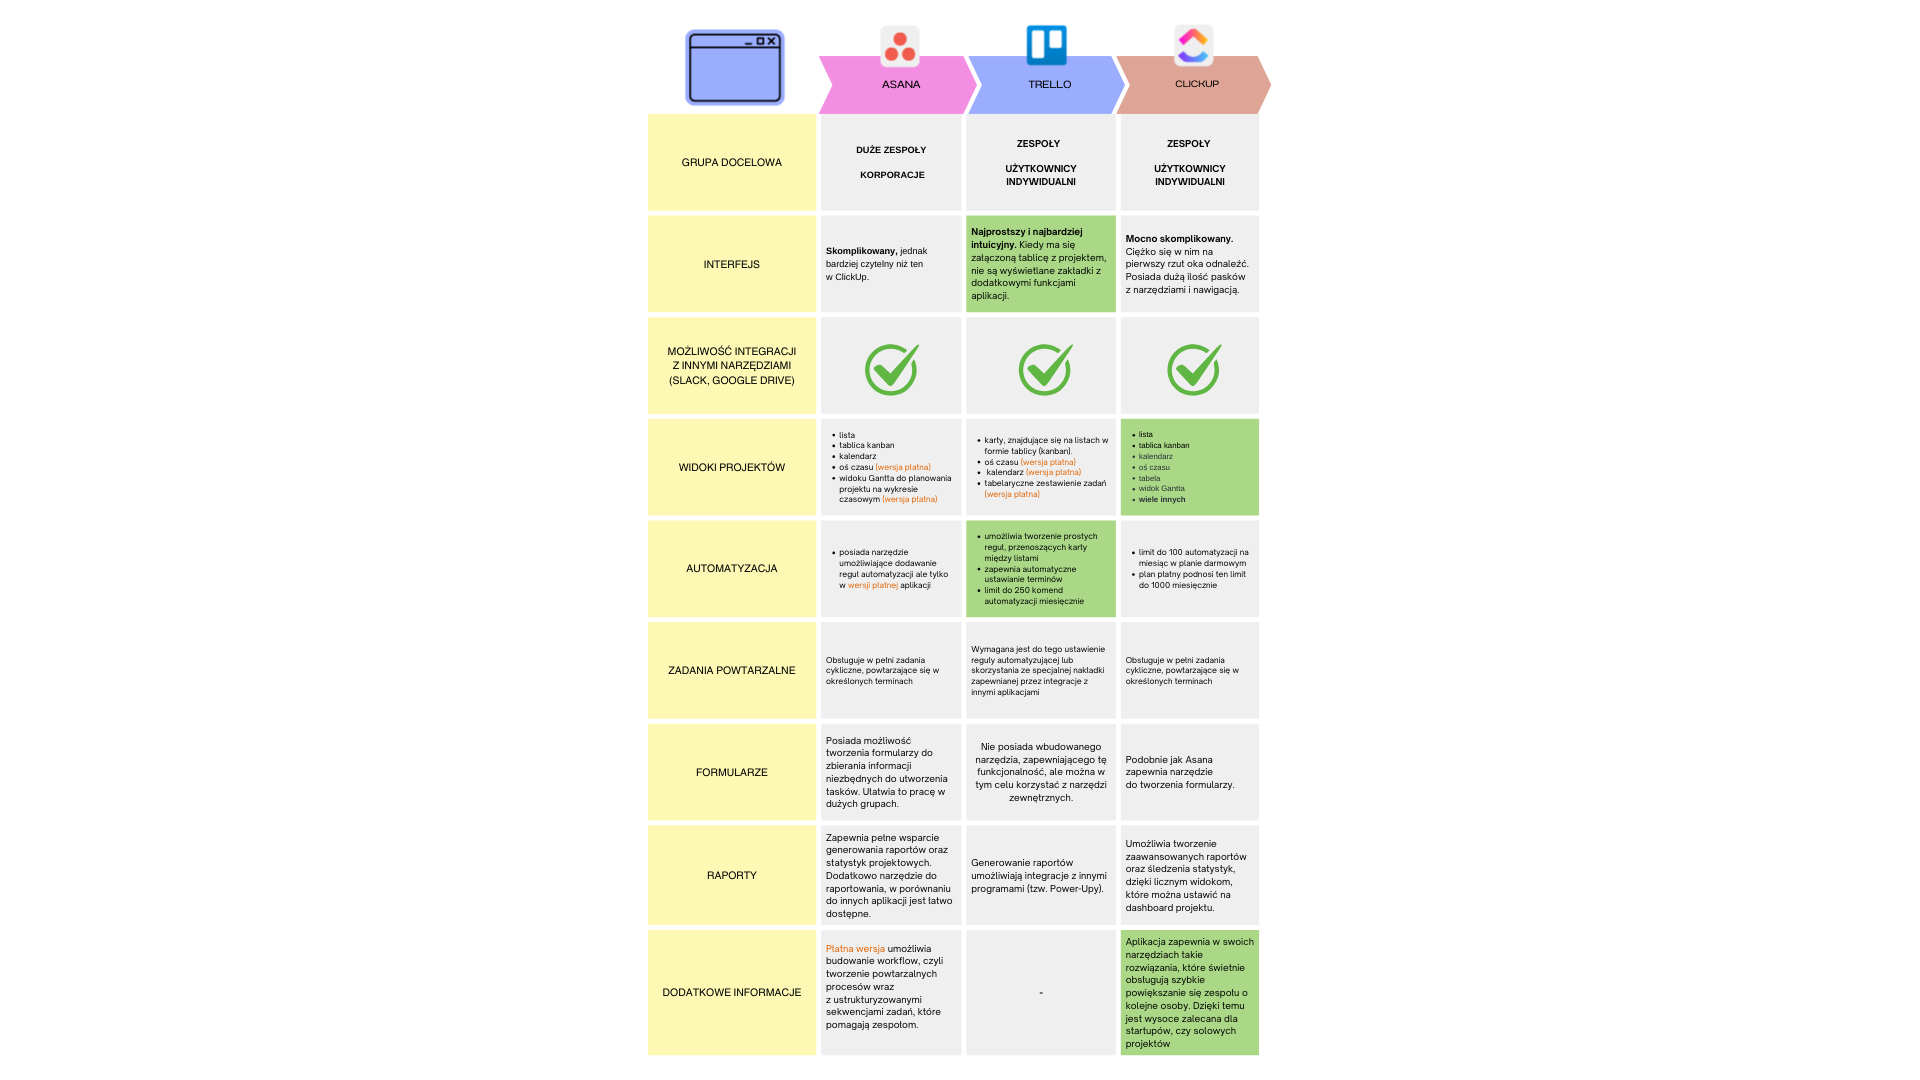
\includegraphics[width=\textwidth]{assets/Porównanie Aplikacji.png}
  \caption{Tabela, porównująca Trello, Asanę oraz ClickUp.}
\end{figure}

Ostateczny wybór zależy od indywidualnych preferencji i potrzeb. Dla typowego użytkownika indywidualnego z prostą listą zadań lub małym projektem Trello może okazać się najwygodniejsze, podczas gdy \textbf{Asana} sprawdzi się tam, gdzie chcemy bardziej formalnie planować projekty. \textbf{ClickUp} będzie najlepszy, w przypadku potrzeby wszechstronnego, elastycznego narzędzia do uporządkowania wielu różnorodnych zadań, w szybko zmieniającym się zespole. Ostatecznie, biorąc pod uwagę użyteczność dla użytkownika indywidualnego, aplikacje ustawiono w kolejności: Trello, ClickUp, Asana.

\section{Historie użytkownika}

\FirstParagraph W procesie projektowania aplikacji internetowej istotne znaczenie ma dokładne zrozumienie potrzeb przyszłych użytkowników oraz sposobu, w jaki będą oni korzystać z systemu. Jedną z powszechnie stosowanych metod opisu wymagań funkcjonalnych są tzw. historie użytkownika, które przedstawiają oczekiwania wobec aplikacji z perspektywy osoby korzystającej z oprogramowania. Takie podejście pozwala skupić się nie na szczegółach implementacyjnych, lecz na rzeczywistych celach i problemach, jakie system ma rozwiązywać.

Historie użytkownika opisują konkretne scenariusze użycia aplikacji w prosty i zrozumiały sposób. Ułatwia to identyfikację kluczowych funkcjonalności systemu, priorytetyzację wymagań oraz projektowanie interfejsu i logiki działania aplikacji zgodnie z rzeczywistymi potrzebami odbiorców. Dodatkowo stanowią one podstawę do planowania implementacji oraz testowania poprawności działania poszczególnych modułów.

Poniżej przedstawiono zestaw pięciu historii użytkownika dla projektowanej aplikacji. Opisują one typowe czynności i odzwierciedlają najważniejsze scenariusze wykorzystania systemu.

\begin{enumerate}
\item
  Jako użytkownik indywidualny, chcę mieć możliwość przypięcia niektórych elementów do strony głównej w celu szybszego dostępu.
\item
  Jako pracownik biurowy, potrzebuję utworzyć kilka zadań wraz z opisami, określonymi priorytetami oraz czasem ich realizacji, w celu efektywniejszej pracy.
\item
  Jako głowa rodziny, potrzebuję utworzyć checklistę zakupów, aby w sklepie niczego nie zapomnieć.
\item
  Jako pracownik nadzorujący dostawy w restauracji, potrzebuję utworzyć notatkę z informacją odnośnie przebiegu dostawy oraz ilości palet zwróconych przez restaurację.
\item
  Jako student potrzebuję utworzyć projekt, zawierający datę realizacji, opis oraz listę podzadań z możliwością nadawania im różnych statusów i wyświetlania w formie tablicy, by nie pogubić się podczas pisania pracy dyplomowej.
\end{enumerate}

Na podstawie powyższych historii użytkownika opracowano szczegółowe scenariusze przypadków użycia, opisujące sposób interakcji użytkownika z systemem w konkretnych sytuacjach. Znajdują się one w szóstym rozdziale pracy.

\section{Kanban}

\FirstParagraph Kanban jest metodą organizacji pracy opartą na wizualnym przedstawianiu zadań oraz etapów ich realizacji. W aplikacjach do zarządzania zadaniami przyjmuje najczęściej postać tablicy podzielonej na kolumny, które odpowiadają kolejnym stanom pracy. Zadania są przedstawiane jako karty, a ich przenoszenie pomiędzy kolumnami pozwala szybko ocenić, które elementy są dopiero planowane, które są aktualnie wykonywane, a które zostały już zakończone.

W literaturze dotyczącej inżynierii oprogramowania kanban jest opisywany jako podejście wspierające ciągły przepływ pracy oraz stopniowe dostarczanie wartości użytkownikowi. Ahmad, Dennehy, Conboy i Oivo wskazują, że badania nad kanbanem w oprogramowaniu koncentrują się między innymi na widoczności pracy, ograniczaniu pracy w toku oraz praktykach usprawniających zarządzanie zadaniami\footnote{Ahmad M. O., Dennehy D., Conboy K., Oivo M., \emph{Kanban in software engineering: A systematic mapping study}, ``Journal of Systems and Software'', vol. 137, 2018, s. 96--113, DOI: 10.1016/j.jss.2017.11.045, \url{https://doi.org/10.1016/j.jss.2017.11.045} (dostęp: 31.07.2026).}.

Zaletą tablicy kanban jest jej prostota. Użytkownik nie musi analizować długiej listy zadań ani otwierać każdego elementu osobno, aby sprawdzić postęp pracy. Wystarczy spojrzeć na układ kart w kolumnach. Dzięki temu metoda dobrze sprawdza się zarówno w pracy zespołowej, jak i w pracy indywidualnej, na przykład podczas planowania projektu, nauki, pisania pracy dyplomowej lub organizowania obowiązków domowych.

Przykładowa tablica kanban może wyglądać następująco:

\begin{table}[H]
  \centering
  \caption{Przykładowa tablica kanban}
  \begin{tabular}{|>{\raggedright\arraybackslash}p{2.55cm}|>{\raggedright\arraybackslash}p{2.55cm}|>{\raggedright\arraybackslash}p{2.55cm}|>{\raggedright\arraybackslash}p{2.55cm}|>{\raggedright\arraybackslash}p{2.55cm}|}
    \hline
    \textbf{Backlog} & \textbf{Do zrobienia} & \textbf{W trakcie} & \textbf{Testowanie} & \textbf{Zrobione} \\
    \hline
    Pomysły na nowe funkcje & Przygotowanie formularza zadania & Implementacja widoku projektu & Sprawdzenie formularza & Konfiguracja logowania \\
    \hline
    Analiza podobnych aplikacji & Dodanie filtrowania zadań & Połączenie z bazą danych & Test działania checklist & Utworzenie modelu użytkownika \\
    \hline
  \end{tabular}
\end{table}

Kolumna \textit{Backlog} przechowuje pomysły lub zadania, które nie zostały jeszcze wybrane do realizacji. Kolumna \textit{Do zrobienia} zawiera elementy zaplanowane jako najbliższe prace. Kolumna \textit{W trakcie} pokazuje zadania aktualnie wykonywane, natomiast \textit{Testowanie} grupuje elementy wymagające sprawdzenia przed uznaniem ich za ukończone. Ostatnia kolumna, \textit{Zrobione}, zawiera zadania zakończone.

W projektowanej aplikacji tablica kanban może zostać wykorzystana przede wszystkim w widoku projektu. Projekt zawiera własne kolumny, a powiązane z nim zadania mogą być przenoszone pomiędzy nimi. Takie rozwiązanie ułatwia kontrolowanie postępu pracy i pozwala użytkownikowi szybko zobaczyć, które zadania wymagają jeszcze uwagi.

\section{Najważniejsze funkcje aplikacji}

\FirstParagraph Wymagania funkcjonalne i niefunkcjonalne stanowią podstawę do opracowania architektury aplikacji, zaprojektowania interfejsu użytkownika oraz implementacji poszczególnych modułów.

Podstawową funkcjonalnością systemu jest umożliwienie użytkownikowi kompleksowego zarządzania elementami organizacyjnymi, którymi są checklisty, notatki, taski oraz projekty. Aplikacja wspiera pełen zestaw operacji CRUD\footnote{CRUD (z jęz. ang. Create, Read, Update, Delete) - zestaw podstawowych operacji wykonywanych na danych w systemach informatycznych, obejmujący ich tworzenie, odczyt, modyfikację oraz usuwanie.}, co pozwala na swobodne dodawanie elementów, ich edycję oraz usuwanie w zależności od potrzeb użytkownika.

Istotnym elementem systemu jest możliwość prezentacji projektów w formie tablicy kanban. Rozwiązanie to pozwala na wizualne przedstawienie stanu realizacji zadań poprzez podział na kolumny, odpowiadające poszczególnym etapom pracy

(np. „w trakcie'', „do zmiany'', „zakończone'', „testowane''). Użytkownik może samodzielnie definiować statusy oraz przenosić zadania pomiędzy kolumnami, co wspiera przejrzyste planowanie i monitorowanie postępów.

Dodatkowo aplikacja udostępnia panel strony głównej (tzw.dashboard), na którym wyświetlane są przypięte przez użytkownika elementy aplikacji, takie jak na przykłąd checklisty. Funkcja ta umożliwia szybki dostęp do najważniejszych informacji bez konieczności przeszukiwania całej aplikacji. System pozwala także na wzbogacanie zadań i projektów o dodatkowe dane, takie jak opis, tagi tematyczne, poziom priorytetu czy przewidywany czas realizacji. Dzięki temu użytkownik może lepiej organizować pracę, filtrować elementy oraz ustalać kolejność wykonywania obowiązków. 

Oprócz funkcjonalności biznesowych istotne znaczenie mają również aspekty jakościowe systemu. Aplikacja umożliwia personalizację poprzez zmianę motywów kolorystycznych oraz przełączanie interfejsu na tryb nocny, co zwiększa komfort użytkowania w różnych warunkach oświetleniowych. Interfejs powinien być minimalistyczny, intuicyjny oraz estetyczny, aby zapewnić łatwość obsługi nawet dla nowych użytkowników.

W zakresie bezpieczeństwa przewidziano integrację z zewnętrznymi dostawcami autentykacji, takimi jak Google i GitHub, co pozwala na bezpieczne logowanie bez konieczności przechowywania haseł w aplikacji. System powinien również zapewniać krótkie czasy ładowania, nieprzekraczające 3--4 sekund dla kluczowych operacji, a także efektywną synchronizację danych w czasie rzeczywistym, umożliwiającą natychmiastowe odświeżanie informacji.

Architektura aplikacji została zaprojektowana w sposób umożliwiający łatwe skalowanie i rozszerzanie funkcjonalności w przyszłości, co pozwala na dalszy rozwój systemu. Dodatkowo przewidziano stosowanie testów jednostkowych i integracyjnych w celu zapewnienia wysokiej jakości oraz niezawodności kodu.

\chapter{Frontend}

\FirstParagraph Frontend\footnote{Frontend - termin pochodzący z języka angielskiego, będący złożeniem słów ``front'' (przód, część widoczna) oraz ``end'' (część, warstwa), odnoszący się do tej części aplikacji, która jest bezpośrednio dostępna dla użytkownika.} to część strony internetowej lub aplikacji, z którą użytkownik bezpośrednio wchodzi w interakcję. Obejmuje on wszystkie akcje, wykonujące się po stronie przeglądarki. Na stronie internetowej do frontendu zalicza się:

\begin{enumerate}
\def\labelenumi{\arabic{enumi}.}
\item
  Układ strony - poszczególne elementy, jak sekcje, nagłówki, przyciski;
\item
  Wygląd strony - czcionki, kolory, animacje;
\item
  Interakcje - wypełnianie formularzy, obsługa klikania elementów strony, menu nawigacyjne;
\item
  Responsywność - automatyczne dostosowywanie się aplikacji do różnych wielkości ekranu.
\end{enumerate}

Fundamentalne narzędzia używane do tworzenia frontendu to HTML\footnote{HTML - z jęz. ang. Hypertext Markup Language, czyli ``hipertekstowy język znaczników''. Dean J., \emph{Web programming with HTML, CSS, and JavaScript}, Burlington 2017.}, CSS\footnote{CSS - z jęz. ang. Cascading Style Sheets, oznaczające ``kaskadujące arkusze stylów''. Dean J., \emph{Web programming with HTML, CSS, and JavaScript}, Burlington 2017.} oraz JavaScript\footnote{JavaScript - język programowania wykorzystywany do tworzenia interaktywnych elementów stron internetowych. Dean J., \emph{Web programming with HTML, CSS, and JavaScript}, Burlington 2017.}. HTML to język znaczników, odpowiadający za strukturę strony internetowej. Określa on semantyczny układ treści, takich jak nagłówki, akapity, listy, obrazy, czy formularze. HTML stanowi szkielet warstwy frontendowej aplikacji webowej, będąc interpretowanym przez przeglądarkę w celu prezentacji treści użytkownikowi. Poprawne i semantyczne rozmieszczenie znaczników HTML ma kluczowe znaczenie dla dostępności cyfrowej, ponieważ umożliwia prawidłową interpretację treści przez czytniki ekranu wykorzystywane przez osoby z niepełnosprawnościami wzroku.

\textbf{CSS} jest językiem służącym do definiowania warstwy prezentacji stron internetowych. Odpowiada za wygląd i układ elementów HTML, w tym kolory, czcionki, odstępy, pozycjonowanie oraz animacje. Dzięki określonemu mechanizmowi dziedziczenia, CSS umożliwia spójne oraz elastyczne zarządzanie stylem w obrębie całej aplikacji webowej, a jego poprawne zastosowanie wspiera czytelność interfejsu oraz dostępność treści dla użytkowników.

\textbf{JavaScript} natomiast jest językiem programowania, umożliwiającym nadanie stronie interaktywności i dynamicznego charakteru. Pozwala na reagowanie na działania użytkownika, modyfikowanie treści oraz struktury dokumentu HTML w czasie rzeczywistym, a także komunikację z serwerem bez konieczności przeładowywania strony. JavaScript stanowi kluczowy element nowoczesnych aplikacji webowych, integrując warstwę prezentacji z logiką działania interfejsu użytkownika.

Wraz ze wzrostem złożoności współczesnych interfejsów użytkownika, wynikła potrzeba rozbudowy i rozszerzania podstawowych technologii frontendowych.

Wczesne zastosowania HTML, CSS i JavaScript ograniczały się głównie do prostych, statycznych stron. Jednak wraz ze wzrostem ilości aplikacji interaktywnych, pojawiła się konieczność lepszej organizacji kodu, ponownego wykorzystania komponentów oraz efektywniejszego zarządzania stanem aplikacji. Dynamiczny rozwój stron internetowych względem ich funkcjonalności i użyteczności zmusił programistów do usprawnienia wcześniej wymienionych języków, w celu sprostania rosnącym oczekiwaniom użytkowników. Biblioteki powstały jako odpowiedź na te wyzwania, umożliwiając realizację dużo bardziej ambitnych i zaawansowanych aplikacji.

Biblioteki programistyczne to zbiory gotowych funkcji, klas oraz komponentów, które rozszerzają możliwości języków programowania i ułatwiają realizację określonych zadań. Ich celem jest ponowne wykorzystanie sprawdzonych rozwiązań, by nie wymyślać koła na nowo. Pozwalają one na skrócenie czasu tworzenia oprogramowania oraz zwiększenie czytelności i niezawodności kodu. W kontekście technologii frontendowych biblioteki wspierają m.in. budowę interfejsu użytkownika, obsługę zdarzeń oraz zarządzanie danymi po stronie klienta.

Przykładem jest tutaj React\footnote{React, \emph{React the library for web and native interfaces}, \url{https://react.dev} (dostęp: 28.01.2026).}, czyli biblioteka języka JavaScript.

Jak można wyczytać na oficjalnej stronie dokumentacji biblioteki, dostarcza ona narzędzia, pozwalająca między innymi na tworzenie komponentów nadających się do ponownego użycia w różnych sekcjach aplikacji. W ten sposób można stworzyć na przykład przycisk, bądź nagłówek, bez potrzeby kilkukrotnego przepisywania kodu, gdy chcemy by nasz dokument HTML zawierał kilka takich samych elementów. Takie podejście nie tylko oszczędza czas, ale również znacznie poprawia przejrzystość kodu. Właśnie z tego powodu w pracy zdecydowano się na skorzystanie z tej biblioteki.

Obok bibliotek, rozwinęło się dużo narzędzi programistycznych zwanych frameworkami\footnote{Framework - z języka angielskiego, jest złożeniem słów ``frame'' (rama) oraz ``work'' (praca, struktura). Dosłownie oznacza "ramę konstrukcyjną" lub "szkielet".}. Różnica pomiędzy biblioteką a frameworkiem dotyczy przede wszystkim stopnia kontroli nad przepływem aplikacji. Biblioteka dostarcza zestaw narzędzi i funkcji, które są wywoływane bezpośrednio przez programistę w wybranym miejscu kodu. Framework natomiast narzuca określoną strukturę projektu oraz sposób działania aplikacji, przejmując kontrolę nad jej przepływem i wymuszając pewne ramy, których programista musi przestrzegać.

\section{Komponenty w React}

\FirstParagraph Komponenty w React stanowią podstawowy element budowy interfejsu użytkownika i umożliwiają podział aplikacji na mniejsze, niezależne moduły. Takie podejście redukuje powielanie kodu oraz ułatwia jego testowanie i utrzymanie. Modułowa struktura aplikacji reactowej zwiększa również skalowalność projektu. Jednak wyżej wspomniane funkcje Reacta nie byłyby możliwe dzięki nakładce do języka JavaScript zwanej JavaScript Extension - w skrócie JSX.

HTML jest językiem deklaratywnym służącym do opisu struktury dokumentu, natomiast JavaScript odpowiada za logikę i manipulację tą strukturą przez wywoływane funkcje.

W klasycznym podejściu HTML i JavaScript są rozdzielone - pierwszy język definiuje widok, a drugi modyfikuje go poprzez interakcję z DOM\footnote{DOM - z jęz. ang. Document Object Model, to hierarchiczna reprezentacja struktury dokumentu HTML w postaci drzewa obiektów. Umożliwia on językom programowania, takim jak JavaScript, dynamiczny dostęp do elementów strony oraz ich modyfikację w czasie działania aplikacji.}.

By zmanipulować DOM'em przy użyciu czystego JavaScriptu należy pierw użyć szeregu przygotowanych przez twórców JSa funkcji. JSX pozwala nam ominąć ten niewygodny oraz czasochłonny proces i pisać wewnątrz plików JavaScripta kod HTML deklaratywnie. To znacznie ułatwia definiowanie, utrzymanie oraz ponowne wykorzystanie komponentów. Dodatkowo składnia JSX jest podczas procesu budowania aplikacji transpilowana do czystego JavaScriptu, dzięki czemu React może efektywnie zarządzać komponentami, ich stanem oraz ponownym wykorzystaniem. Poniższy przykład wyjaśnia, jak w React działa JavaScript Extension.

\begin{figure}[H]
  \centering
  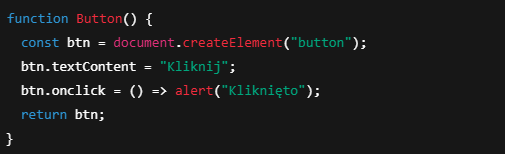
\includegraphics[width=4.98233in,height=1.52294in]{imported-media/media/image2.png}
  \caption{Fragment kodu przedstawiający definiowanie komponentu Button w czystym JavaScript, bez nakładki JSX}
\end{figure}

Jak widać na wyżej zamieszczonej grafice, w czystym JavaScripcie komponent można zbudować wyłącznie poprzez imperatywne tworzenie elementów. Takie podejście jest mało czytelne, trudne w utrzymaniu i nie skaluje się dobrze w przypadku złożonych interfejsów.

\begin{figure}[H]
  \centering
  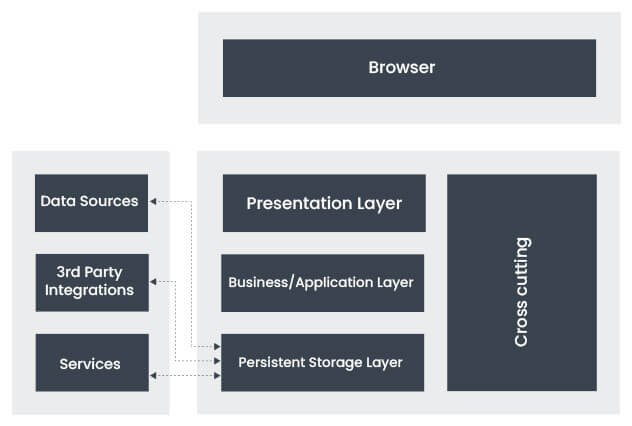
\includegraphics[width=5.66892in,height=0.80294in]{imported-media/media/image3.png}
  \caption{Fragment kodu przedstawiający deklaratywne definiowanie komponentu Button dzięki JSX}
\end{figure}

Wyżej przedstawiono, jak prosto w sposób deklaratywny dodaje się elementy HTMLa, dzięki bibliotece React. W React wyróżnia się dwa podstawowe typy komponentów - klasowe oraz funkcyjne, różniące się zarówno składnią, jak i sposobem zarządzania logiką aplikacji. Komponenty klasowe opierają się na klasach wprowadzonych do JavaScript wraz z aktualizacją ES6\footnote{ES6 - skrót od ``ECMAScript 2015'', jest to szósta edycja standardu języka JavaScript, która znacząco rozszerzyła możliwości języka.}. Dziedziczą one po klasie \textbf{React.Component}, a zarządzanie stanem oraz cyklem życia komponentu odbywa się za pomocą metod takich jak \textbf{constructor}, \textbf{componentDidMount}, czy \textbf{componentDidUpdate}. Taki model prowadzi często do bardziej rozbudowanego i mniej czytelnego kodu, zwłaszcza w przypadku złożonych komponentów. Poniżej widnieje przykład komponentu klasowego o nazwie ``Button''. Komponent ten renderuje przycisk, którego treść oraz obsługa zdarzenia kliknięcia są przekazywane z zewnątrz za pomocą parametru ``props'', co jest standardem zarówno jeśli chodzi o komponenty klasowe jak i funkcyjne.

\begin{figure}[H]
  \centering
  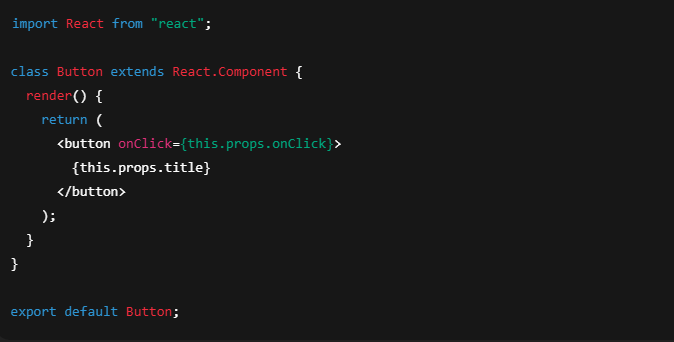
\includegraphics[width=5.29087in,height=2.6833in]{imported-media/media/image4.png}
  \caption{Fragment kodu przedstawiający klasowy komponent ``Button''}
\end{figure}

Jeśli chodzi o komponenty funkcyjne, to są one zwykłymi funkcjami JavaScript, przyjmującymi dane wejściowe za pomocą ``props'' i zwracają strukturę interfejsu użytkownika. Początkowo były one ograniczone do komponentów prezentacyjnych, jednak wprowadzenie mechanizmu React Hooks rozszerzyło ich zastosowanie do pełnoprawnych elementów logiki aplikacji. Dzięki prostszej składni i lepszej modularności komponenty funkcyjne są obecnie preferowanym i rekomendowanym podejściem w nowoczesnych aplikacjach.

Poniżej zamieszczono przykład tego samego komponentu ``Button'', lecz w formie funkcji.

\begin{figure}[H]
  \centering
  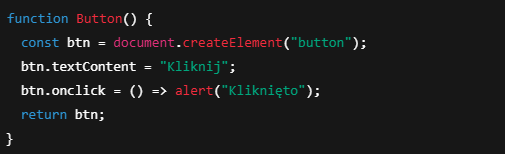
\includegraphics[width=4.61253in,height=2.52232in]{imported-media/media/image5.png}
  \caption{Fragment kodu przedstawiający funkcyjny komponent ``Button''}
\end{figure}

\section{React Hooks}

\FirstParagraph Mechanizm hooków umożliwia przechowywanie danych pomiędzy kolejnymi wywołaniami funkcji komponentu, mimo że sama funkcja jest wykonywana od nowa przy każdym renderowaniu. Każdy hook jest wywoływany bezpośrednio w ciele funkcji komponentu, dzięki czemu React może jednoznacznie przypisać jego działanie do danego komponentu oraz zachować odpowiednie wartości pomiędzy kolejnymi wywołaniami tej funkcji. Kolejność wywołań hooków ma kluczowe znaczenie, ponieważ na jej podstawie React identyfikuje, które dane należą do danego hooka.

W odróżnieniu od zwykłych zmiennych lokalnych, które są tracone po zakończeniu wykonania funkcji, wartości zarządzane przez hooki są przechowywane poza samą funkcją, lecz udostępniane jej ponownie przy każdej aktualizacji interfejsu użytkownika. Dzięki temu komponent funkcyjny może być ponownie wykonywany, zachowując ciągłość danych oraz logiki aplikacji.

W JavaScripcie zasięg funkcji określa obszar kodu, w którym dana zmienna lub funkcja jest dostępna. W przypadku komponentów funkcyjnych oznacza to, że wszystkie zmienne, Hooki oraz funkcje pomocnicze zadeklarowane wewnątrz komponentu są dostępne wyłącznie w obrębie jego ciała. Zapewnia to, że stan oraz logika komponentu pozostają hermetyczne i nie kolidują z innymi komponentami, co sprzyja modularności, przewidywalności oraz bezpieczeństwu struktury aplikacji.

Zarządzanie stanem aplikacji w komponencie polega na przechowywaniu oraz aktualizowaniu danych, które mają bezpośredni wpływ na wyświetlany interfejs użytkownika. Stan reprezentuje bieżące parametry komponentu, takie jak wartości formularza, licznik, widoczność elementów, czy dane pobrane z serwera. Zmiana stanu powoduje ponowną aktualizację widoku komponentu w celu odzwierciedlenia nowych danych.

W komponentach funkcyjnych, stan jest obsługiwany za pomocą specjalnej funkcji, składającej się z aktualnej wartości stanu oraz metody służącej do jej zmiany. Funkcja ta nie modyfikuje stanu bezpośrednio, lecz informuje Reacta o konieczności jego aktualizacji.

\begin{figure}[H]
  \centering
  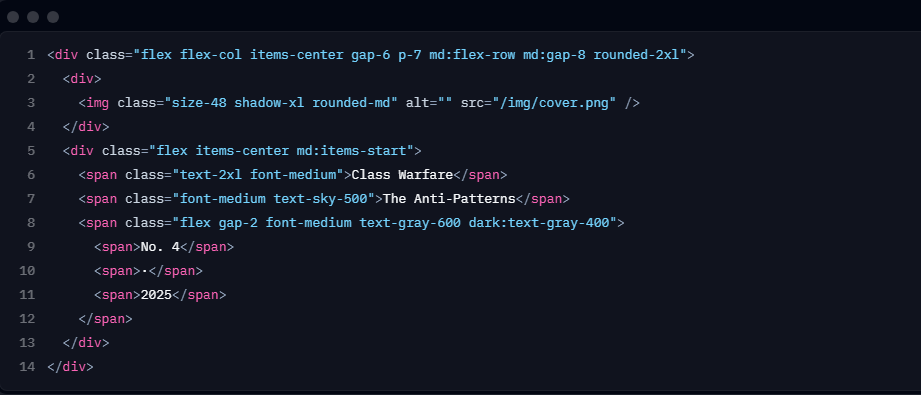
\includegraphics[width=5.83952in,height=3.23864in]{imported-media/media/image6.png}
  \caption{Przykład funkcji zarządzającej stanem komponentu ``Counter''}
\end{figure}

W powyższym przykładzie:

\begin{itemize}
\item
  zmienna \textbf{count} przechowuje aktualny stan licznika,
\item
  funkcja \textbf{setCount} odpowiada za aktualizację stanu,
\item
  wywołanie funkcji setCount powoduje zmianę danych oraz odświeżenie widoku komponentu na stronie
\end{itemize}

Takie podejście zapewnia enkapsulację danych wewnątrz komponentu oraz precyzyjne sterowanie jego zachowaniem. Dzięki hookom zarządzanie stanem staje się czytelne i ściśle powiązane z zakresem funkcji komponentu, co ułatwia rozwój i utrzymanie aplikacji.

\section{TailwindCSS}

\FirstParagraph TailwindCSS\footnote{Tailwind Labs, \emph{Tailwind CSS}, \url{https://tailwindcss.com} (dostęp: 28.01.2026).} jest frameworkiem służącym do stylowania interfejsów użytkownika za pomocą gotowych klas CSS, używanych bezpośrednio w znacznikach HTML lub komponentach Reactowych. Tailwind umożliwia szybkie budowanie spójnych i responsywnych layoutów bez konieczności pisania własnych arkuszy stylów dla każdego komponentu. Technologia ta jest stosowana w celu zwiększenia produktywności, ograniczenia duplikacji kodu CSS oraz łatwiejszego skalowania warstwy prezentacyjnej aplikacji.

\begin{figure}[H]
  \centering
  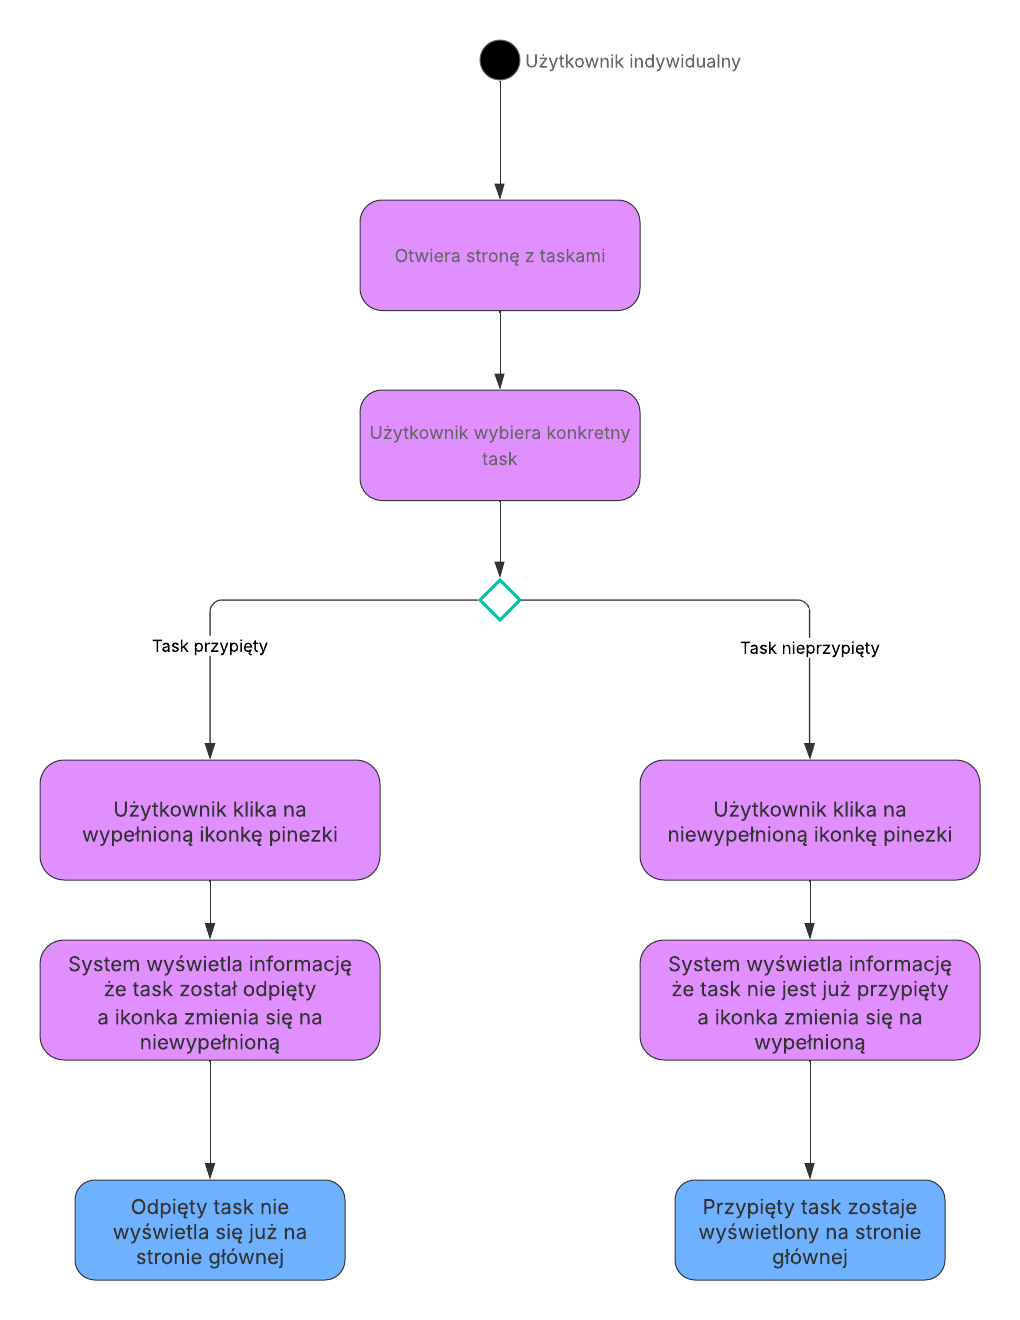
\includegraphics[width=6.10236in,height=2.61111in]{imported-media/media/image7.png}
  \caption{Przykładowe użycie TailwindCSS, pochodzące z oficjalnej strony frameworka (dostęp: 28.01.2026)}
\end{figure}

Jak widać na obrazie, całe stylowanie realizowane jest poprzez tak zwane klasy narzędziowe (po angielsku utility classes) Tailwinda, bez użycia osobnych plików CSS.

Dla przykładu - klasa ``flex''nadana znacznikowi ``div'' w piątej linijce kodu, jest tożsama z CSSowym ``display: flex;''. W projekcie aplikacji omawianej w niniejszej pracy, Tailwinda użyto, z następujących powodów:

\begin{itemize}
\item
  dzięki niemu nie trzeba definiować własnych klas CSS,
\item
  umożliwia szybkie tworzenie responsywnych i spójnych komponentów,
\item
  eliminuje potrzebę przechodzenia do osobnych plików stylów w celu sprawdzenia struktury wizualnej znacznika lub komponentu.
\end{itemize}

\section{TypeScript}

\FirstParagraph Kolejną technologią zastosowaną w projekcie jest TypeScript\footnote{Microsoft, \emph{TypeScript Documentation}, \url{https://www.typescriptlang.org/docs/} (dostęp: 25.07.2026).}, czyli nadzbiór języka JavaScript. Rozszerza on JSa o system typów, interfejsy oraz mechanizmy kontroli poprawności kodu na etapie kompilacji. Kod TypeScript nie jest bezpośrednio interpretowany przez przeglądarkę, lecz przed uruchomieniem musi zostać transpilowany do standardowego JavaScriptu, zachowując pełną kompatybilność ze środowiskiem wykonawczym.

Głównym celem stosowania TypeScript jest zwiększenie bezpieczeństwa, czytelności oraz przewidywalności kodu. Statyczne typowanie pozwala wykrywać błędy już na etapie pisania kodu a nie podczas działania aplikacji. TypeScript znacząco ułatwia pracę w dużych projektach oraz zespołach programistycznych, ponieważ jasno definiuje struktury danych oraz oczekiwane typy argumentów. Ponadto redukuje ryzyko błędów logicznych trudnych do wykrycia w czystym JavaScripcie i dobrze integruje się z nowoczesnymi frameworkami frontendowymi.

Brak TypeScriptu w większych aplikacjach pisanych w JavaScript może prowadzić do szeregu problemów. Przykładowo, JS pozwala na swobodne przekazywanie danych dowolnego typu, co może skutkować błędami w czasie działania aplikacji, np. wywołaniem metod na nieprawidłowym typie danych. Również wiele problemów, takich jak błędnie zapisane wyrazy w nazwach pól obiektów, czy nieprawidłowe argumenty funkcji, ujawnia się dopiero podczas działania aplikacji. W czystym JavaScripcie brakuje też mechanizmu, wymuszającego spójność zmian w całym projekcie, przez co zmiana struktury danych wiąże się z większym ryzykiem niezamierzonych błędów. Jednak najważniejszą cechą projektów, wykorzystujących TypeScript jest zdecydowanie dużo wyższa czytelność i przewidywalność kodu. Jawnie zdefiniowane typy ułatwiają zrozumienie, jakie dane są przetwarzane przez funkcje oraz komponenty, co znacznie wpływa na utrzymanie aplikacji oraz wdrażanie nowych programistów do projektu.

Jak dokładnie działa TypeScript można wytłumaczyć na następującym przykładzie. Tworzony jest komponent odpowiedzialny za wyświetlanie na stronie danych użytkownika - takich jak imię, adres e-mail oraz wiek. W TypeScripcie definiowany jest typ lub interfejs, który jednoznacznie określa, jaką strukturę muszą mieć parametry przyjmowane przez komponent - n.p. imię i adres e-mail muszą być zmienną typu ``string'', a wiek - ``number''. Następnie komponent lub funkcja przyjmująca dane użytkownika deklaruje, że oczekuje dokładnie takiego typu danych. Dzięki temu TypeScript już na etapie pisania kodu sprawdza, czy przekazywane wartości są poprawne. Jeżeli programista spróbuje przekazać zmienną typu ``number'' zamiast ``string'' lub pominie wymagane pole, błąd zostanie wykryty jeszcze przed uruchomieniem aplikacji. W trakcie dalszego rozwoju projektu, gdy struktura danych użytkownika ulegnie zmianie, TypeScript automatycznie wskaże wszystkie miejsca w aplikacji, które wymagają aktualizacji. Zintegrowane środowiska programistyczne\footnote{Zintegrowane środowisko programistyczne - w skrócie IDE, to zestaw narzędzi oraz konfiguracji wykorzystywanych do tworzenia oprogramowania, obejmujący m.in. edytor lub środowisko IDE}, posiadają możliwość integracji z TypeScriptem poprzez wyświetlanie na bieżąco powiadomień i ostrzeżeń o potencjalnych błędach wykrywanych przez ten język.

\chapter{Backend}

\FirstParagraph Backend\footnote{Backend - termin pochodzący z języka angielskiego, będący złożeniem słów ``back'' (tył, zaplecze) oraz ``end'' (część, warstwa), odnoszący się do części aplikacji niedostępnej dla użytkownika.} to warstwa aplikacji działająca po stronie serwera i odpowiedzialna za przetwarzanie danych oraz komunikację z bazą danych lub innymi systemami. Backend nie jest bezpośrednio widoczny dla użytkownika końcowego. Obsługuje m.in. autoryzację, walidację\footnote{Walidacja - proces sprawdzania poprawności, kompletności oraz zgodności danych wejściowych z określonymi regułami i wymaganiami systemu.} danych, realizację reguł biznesowych oraz udostępnianie danych frontendowi za pomocą API\footnote{API - skrót z języka angielskiego, oznaczający Application Programming Interface.}.

API natomiast to zestaw reguł, metod i struktur danych umożliwiających komunikację pomiędzy różnymi systemami informatycznymi lub ich częściami. Określa, w jaki sposób aplikacje mogą wymieniać dane oraz wywoływać określone funkcje, bez konieczności znajomości wewnętrznej implementacji drugiej strony. API pełni rolę pośrednika pomiędzy frontendem a backendem. Frontend wysyła żądania lub zapytania, natomiast backend przetwarza je, zwracając później odpowiedź.

\section{Next.js}

\FirstParagraph Next.js\footnote{Vercel, \emph{Next.js Docs}, \url{https://nextjs.org/docs} (dostęp: 29.01.2026).} jest frameworkiem opartym na bibliotece React, przeznaczonym do tworzenia pełnostosowych aplikacji webowych. Interfejs użytkownika budowany jest przy użyciu komponentów Reacta, natomiast Next.js dostarcza dodatkowe funkcje oraz mechanizmy optymalizacyjne. Framework automatycznie konfiguruje narzędzia niskiego poziomu, takie jak bundlery oraz kompilatory, dzięki czemu programista może skupić się na tworzeniu aplikacji i szybkim wdrażaniu jej do użytku.

Next.js rozszerza możliwości Reacta o funkcje takie jak renderowanie zawartości po stronie serwera, routing\footnote{Routing - mechanizm zarządzania nawigacją w aplikacji, umożliwiający użytkownikowi poruszanie się pomiędzy różnymi częściami systemu.} oparty na strukturze plików, optymalizację obrazów oraz wygodne tworzenie endpointów API. Umożliwia również budowę aplikacji przyjaznych dla wyszukiwarek internetowych, ponieważ część treści może zostać przygotowana przed wysłaniem strony do przeglądarki. Dzięki temu framework łączy w jednym projekcie warstwę interfejsu użytkownika i wybrane mechanizmy backendowe.

W projekcie zdecydowano się na wykorzystanie Next.js, ponieważ framework ogranicza potrzebę utrzymywania osobnego projektu backendowego i ułatwia rozwijanie aplikacji jako jednej spójnej całości. Najważniejsze znaczenie miały routing oparty na strukturze plików, możliwość tworzenia endpointów API w tym samym repozytorium oraz wsparcie dla różnych strategii renderowania. Istotne było także proste połączenie z Auth.js\footnote{Auth.js, \emph{Auth.js}, \url{https://authjs.dev} (dostęp: 17.07.2026).}, które pozwala zabezpieczać widoki i endpointy bez tworzenia całego mechanizmu logowania od podstaw.

Dodatkową zaletą Next.js jest wsparcie dla SEO, w tym lepszej indeksowalności strony\footnote{Indeksowalność strony - cecha strony internetowej oznaczająca, że jej treść może zostać poprawnie odczytana, zinterpretowana i umieszczona w indeksie wyszukiwarki internetowej.} dzięki renderowaniu treści po stronie serwera oraz możliwości zarządzania metadanymi dokumentu. Dla aplikacji do organizacji zadań znaczenie ma również wygoda rozwijania widoków użytkownika i kodu serwerowego w tym samym środowisku technologicznym.

\section{Routing}

\FirstParagraph Routing w Next.js stanowi mechanizm odpowiedzialny za mapowanie adresów URL na konkretne widoki aplikacji. W przeciwieństwie do klasycznych aplikacji React, w których konfiguracja tras wymaga dodatkowych bibliotek i ręcznego definiowania reguł nawigacji, Next.js wykorzystuje routing oparty na strukturze plików - z jęz. ang. file-based routing. Ścieżki URL są automatycznie generowane na podstawie organizacji katalogów i plików w projekcie.

Podstawową zasadą działania tego mechanizmu, jest przypisanie każdemu plikowi
 w katalogu pages lub app, odpowiadającej mu trasy. Przykładowo - plik ``about.js'' generuje ścieżkę ``/about'', natomiast plik umieszczony w podkatalogu ``blog/post.js'', odpowiada adresowi ``/blog/post''. Takie rozwiązanie upraszcza konfigurację projektu, zwiększa czytelność struktury aplikacji oraz ogranicza konieczność tworzenia dodatkowych plików konfiguracyjnych.

Next.js obsługuje również routing dynamiczny, który umożliwia tworzenie stron
 o zmiennych parametrach, np. dla wpisów blogowych czy profili użytkowników. Realizowane jest to poprzez specjalną składnię nazw plików, co pozwala na generowanie wielu widoków na podstawie jednego szablonu komponentu. Aby utworzyć dynamiczną ścieżkę, zmieniającą się w zależności od parametru ``id'' użytkownika, należy w katalogu ``users'' utworzyć plik o nazwie {[}id{]}.js. Wewnątrz komponentu parametr ``id'' można odczytać ze specjalnego obiektu routingu. Przykładowo, pojedynczy komponent może generować widok profilu na podstawie identyfikatora przekazanego w adresie URL. Takie podejście pozwala na tworzenie wielu stron przy użyciu jednego szablonu, co zwiększa modularność oraz skalowalność aplikacji.

Dodatkowo framework wspiera nawigację po stronie klienta, realizowaną za pomocą komponentu ``Link'', dzięki czemu przejścia pomiędzy stronami odbywają się bez pełnego przeładowania dokumentu. Rozwiązanie to zwiększa wydajność oraz poprawia płynność działania interfejsu użytkownika.

Zastosowanie wbudowanego systemu routingu w Next.js upraszcza proces tworzenia aplikacji, redukuje ilość kodu konfiguracyjnego oraz sprzyja zachowaniu spójnej i logicznej struktury projektu, co ma istotne znaczenie w większych i długoterminowych przedsięwzięciach programistycznych.

\section{Generowanie zawartości strony}

\FirstParagraph Domyślnie Next.js używa serwerowych komponentów Reacta. Wykonują się one najpierw po stronie serwera, a następnie ich wynik wysyłany jest do klienta.

Komponenty te zapewniają wsparcie dla JSowych obiektów typu Promise, umożliwiających wykonywanie zadań asynchronicznych bez konieczności używania dodatkowych bibliotek czy hooków Reactowych. Natomiast pobieranie danych zawsze odbywa się asynchronicznie. Ponieważ komponenty serwerowe działają po stronie serwera, możliwe jest bezpośrednie wykonywanie zapytań do bazy danych bez konieczności korzystania z dodatkowej warstwy API. Pozwala to ograniczyć ilość kodu, który trzeba pisać i utrzymywać.

Pobrane dane można generować i przetwarzać na dwa różne sposoby. Renderowanie statyczne polega na generowaniu treści na etapie budowania aplikacji lub podczas jej ponownej walidacji, a następnie dostarczaniu gotowych stron użytkownikom, co zwiększa wydajność i zmniejsza obciążenie serwera oraz sprzyja optymalizacji SEO\footnote{SEO (z jęz. ang. Search Engine Optimization) -- proces optymalizacji stron internetowych, mający na celu poprawę ich widoczności w wynikach wyszukiwarek internetowych poprzez dostosowanie treści, struktury oraz wydajności serwisu do wymagań algorytmów indeksujących.}. Renderowanie dynamiczne natomiast, odbywa się przy każdym żądaniu użytkownika, umożliwiając prezentację danych aktualnych w czasie rzeczywistym. Pierwsze podejście sprawdza się w przypadku stron o stałej zawartości, natomiast drugie jest preferowane w aplikacjach, wymagających częstych aktualizacji danych, takich jak panele administracyjne czy profile użytkowników.

Buforowanie danych polega na tymczasowym przechowywaniu wyników wcześniej wykonanych operacji, takich jak zapytania do bazy danych lub odpowiedzi z API, w celu ich wykorzystania bez konieczności ponownego przetwarzania. Dzięki temu kolejne żądania mogą zostać obsłużone szybciej, ponieważ dane są odczytywane z pamięci podręcznej zamiast generowane od podstaw. Mechanizm ten zmniejsza obciążenie serwera, skraca czas odpowiedzi aplikacji oraz poprawia ogólną wydajność systemu.

Równie istotnym elementem optymalizacji w Next.js, jest deduplikacja zapytań, czyli eliminacja wielokrotnego pobierania tych samych danych. Jeżeli kilka komponentów wymaga tych samych informacji, system wykonuje zapytanie tylko raz, a następnie współdzieli wynik pomiędzy wszystkimi. Zmniejsza to obciążenie serwera, skraca czas odpowiedzi oraz poprawia efektywność wykorzystania zasobów, co ma szczególne znaczenie w rozbudowanych aplikacjach.

\section{API w Next.js}

\FirstParagraph Ścieżki API w Next.js to mechanizm, umożliwiający definiowanie punktów końcowych\footnote{Punkt końcowy - reprezentowany jest przez określony adres URL oraz metodę HTTP, udostępniając konkretną funkcjonalność lub zasób systemu. Umożliwia komunikację pomiędzy klientem a serwerem.} API bezpośrednio w projekcie Next.js. Endpointy (z jęz. ang. punkty końcowe) można tworzyć poprzez umieszczenie plików w katalogu ``pages/api'', a każda taka funkcja obsługuje żądania HTTP i zwraca odpowiedź w modelu ``request/response''\footnote{Interfejs typu request/response -- model komunikacji pomiędzy klientem a serwerem, w którym klient wysyła żądanie (request) zawierające określone dane lub operację, a serwer przetwarza je i zwraca odpowiedź (response) z wynikiem działania, danymi lub informacją o błędzie.}.

W nowszym podejściu, odpowiednikiem ścieżek API są tzw. "Route Handlers" (z jęz. ang. obsługa ścieżek), definiowane w katalogu ``app'' i pliku ``route.js''. W tym modelu obsługa metod HTTP realizowana jest przez eksport funkcji takich jak ``GET'', ``POST'', ``PUT'' czy ``DELETE'', co pozwala tworzyć endpointy w sposób bardziej zbliżony do standardowych interfejsów typu ``request/response''.

Zastosowanie API Routes obejmuje m.in. obsługę formularzy, operacje CRUD, integracje z usługami zewnętrznymi, czy realizację logiki po stronie serwera, która nie powinna być wykonywana w przeglądarce. Istotną zaletą jest fakt, że kod endpointów nie trafia do klienta, dzięki czemu możliwe jest bezpieczniejsze przetwarzanie danych oraz użycie zmiennych środowiskowych po stronie serwera.

W projektowanej aplikacji endpointy API pełnią rolę kontrolowanej bramy pomiędzy interfejsem użytkownika a bazą danych. To po ich stronie możliwe jest sprawdzenie sesji użytkownika, walidacja przesłanych danych, odrzucenie niepoprawnego żądania oraz wykonanie zapisu lub odczytu w bazie. Dzięki temu frontend nie musi znać szczegółów działania modeli danych, a użytkownik nie otrzymuje bezpośredniego dostępu do warstwy przechowywania informacji.

Takie podejście ułatwia również utrzymanie spójności logiki biznesowej. Jeżeli kilka widoków aplikacji korzysta z tej samej operacji, na przykład tworzenia zadania albo aktualizowania checklisty, reguły tej operacji mogą zostać zapisane w jednym handlerze API. Zmniejsza to ryzyko rozbieżności między widokami oraz upraszcza późniejsze testowanie zachowania systemu.

\section{Autoryzacja i autentykacja}

\FirstParagraph W Next.js autentykację i autoryzację można wdrożyć poprzez integrację z dostawcą OAuth\footnote{OAuth - z jęz. ang. Open Authorization, to standard protokołu autoryzacji umożliwiający aplikacjom uzyskanie dostępu do zasobów użytkownika w innym systemie bez konieczności przekazywania jego hasła. Zamiast tego wykorzystywane są specjalne tokeny dostępu, które określają zakres przyznanych uprawnień.} przy użyciu biblioteki Auth.js. Rozwiązanie to pozwala skonfigurować logowanie przez zewnętrznych dostawców, takich jak Google, czy Github. Biblioteka automatycznie obsługuje sesje użytkownika, przekazywanie tokenów oraz proces powrotu użytkownika do aplikacji po zakończonym logowaniu.

Autentykacja polega na potwierdzeniu tożsamości użytkownika, natomiast autoryzacja określa, do jakich zasobów i operacji użytkownik ma dostęp po zalogowaniu. W aplikacji do zarządzania zadaniami rozróżnienie to ma duże znaczenie, ponieważ samo zalogowanie użytkownika nie powinno jeszcze oznaczać dostępu do cudzych projektów, checklist, notatek lub tasków.

Po zalogowaniu aplikacja może kontrolować dostęp do zasobów na podstawie informacji z sesji, np. identyfikatora użytkownika, ról lub uprawnień. W praktyce każdy endpoint obsługujący dane powinien sprawdzać, czy żądanie pochodzi od zalogowanego użytkownika oraz czy wskazany dokument należy właśnie do niego. Pozwala to ograniczyć dostęp do wybranych stron i endpointów API oraz zmniejsza ryzyko nieautoryzowanej modyfikacji danych.

\chapter{Bazy Danych}

\FirstParagraph Baza danych to system służący do trwałego przechowywania, organizowania oraz zarządzania danymi, wykorzystywanymi przez aplikację. Umożliwia ona zapisywanie informacji w ustrukturyzowanej formie, ich wyszukiwanie, modyfikację oraz usuwanie, zapewniając jednocześnie spójność, integralność i bezpieczeństwo przechowywanych informacji. Najczęściej stosuje się bazy relacyjne lub nierelacyjne, w zależności od charakteru przetwarzanych danych.

Relacyjne bazy danych to systemy, przechowujące dane w postaci tabel, składających się z wierszy i kolumn, powiązanych ze sobą za pomocą relacji. Wykorzystują one ustrukturyzowany schemat danych oraz język zapytań SQL (Structured Query Language), co zapewnia wysoką spójność i integralność informacji. Sprawdzają się szczególnie w aplikacjach, które wymagają precyzyjnych zależności między danymi.

Bezrelacyjne bazy danych, zwane bazami noSQL, przechowują dane w bardziej elastycznej formie. Mogą to na przykład być dokumenty, pary klucz--wartość, grafy lub kolekcje. Takie bazy nie wymagają sztywno zdefiniowanego schematu, co ułatwia skalowanie oraz pracę z dużymi i zróżnicowanymi zbiorami danych.

W architekturze aplikacji internetowej baza danych współpracuje przede wszystkim z warstwą backendową. Backend realizuje zapytania do bazy, przetwarza otrzymane wyniki zgodnie z logiką biznesową, a następnie udostępnia je frontendowi za pośrednictwem interfejsów API. Frontend odpowiada za prezentację danych, jednak nie komunikuje się bezpośrednio z bazą. Takie rozdzielenie odpowiedzialności zwiększa bezpieczeństwo systemu, ułatwia utrzymanie kodu oraz pozwala na skalowanie poszczególnych warstw aplikacji niezależnie od siebie.

\begin{figure}[H]
  \centering
  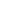
\includegraphics[width=5.7792in,height=2.98542in]{imported-media/media/image8.png}
  \caption[Przedstawienie procesu wyświetlania danych użytkownikowi aplikacji internetowej]{Przedstawienie procesu, umożliwiającego wyświetlenie danych użytkownikowi aplikacji internetowej. Źródło: \url{https://d1zruf9db62p8s.cloudfront.net/2025/08/Frontend-vs-Backend.webp} (dostęp: 02.02.2026).}
\end{figure}

\section{MySQL}

\FirstParagraph MySQL\footnote{Oracle, \emph{MySQL Documentation}, \url{https://dev.mysql.com/doc/} (dostęp: 25.07.2026).} należy do najczęściej wykorzystywanych technologii bazodanowych w aplikacjach internetowych ze względu na wysoką wydajność, stabilność, łatwość konfiguracji oraz szerokie wsparcie społeczności i narzędzi programistycznych. Ten typ bazy danych wykorzystuje język SQL do definiowania struktury danych, wykonywania zapytań oraz zarządzania integralnością informacji.

Dane w MySQL przechowywane są w tabelach złożonych z wierszy -- tak zwanych rekordów i kolumn, zwanych atrybutami. Relacje pomiędzy tabelami realizowane są za pomocą kluczy głównych i obcych, co pozwala zachować spójność danych oraz minimalizować redundancję\footnote{Redundancja - nadmiarowość danych, polegająca na wielokrotnym przechowywaniu tych samych informacji w różnych miejscach systemu.}. Klucz główny to kolumna lub zestaw kolumn, których wartość jednoznacznie identyfikuje każdy rekord w tabeli. Wartości klucza głównego muszą być unikalne i nie mogą przyjmować wartości pustych (wartości null). Natomiast klucz obcy to kolumna lub zestaw kolumn w tabeli, odwołujący się do klucza głównego w innej tabeli. Służy on do tworzenia powiązań między danymi, np. przypisania zamówienia do konkretnego użytkownika. Mechanizm kluczy obcych wymusza spójność relacyjną, zapobiegając wprowadzaniu odwołań do nieistniejących rekordów. MySQL obsługuje transakcje, indeksowanie oraz mechanizmy buforowania, co zapewnia bezpieczne i szybkie operacje odczytu oraz zapisu.

Backend aplikacji komunikuje się z bazą poprzez zapytania, pobierając lub modyfikując dane, a następnie przekazuje je do warstwy frontendowej za pośrednictwem interfejsów API. Takie podejście oddziela logikę biznesową od warstwy prezentacji oraz zwiększa bezpieczeństwo systemu. Do kluczowych funkcjonalności mySQL należą:

\begin{itemize}
\item
  obsługa zapytań, takich jak SELECT, INSERT, UPDATE, DELETE, realizujących operacje na danych,
\item
  transakcje - odpowiedzialne za wykonywanie kilku różnych operacji na bazie danych jednocześnie, układając je w jedną logiczną całość,
\item
  indeksy - unikalnie identyfikują i przyspieszają wyszukiwanie rekordów,
\item
  tworzenie widoków, czyli wirtualnych tabel, upraszczających złożone zapytania,
\item
  procedury składowane i wyzwalacze, służące do automatyzowania operacji po stronie bazy danych,
\item
  zarządzanie użytkownikami, uprawnieniami oraz szyfrowaniem połączeń.
\end{itemize}

Dzięki swojej niezawodności oraz dobrej integracji z popularnymi technologiami backendowymi mySQL stanowi uniwersalne i efektywne rozwiązanie dla aplikacji wymagających uporządkowanego modelu danych oraz wysokiej spójności informacji. System ten doskonale sprawdza się w aplikacjach administracyjnych, systemach rezerwacji, portalach społecznościowych, czy sklepach internetowych.

\section{MongoDB}

\FirstParagraph MongoDB\footnote{MongoDB, Inc., \emph{Welcome to the MongoDB docs}, \url{https://www.mongodb.com/docs/} (dostęp: 02.02.2026).} jest nierelacyjnym systemem zarządzania bazą danych, którego podstawową różnicą względem relacyjnych rozwiązań, jest sposób przechowywania informacji. MongoDB wykorzystuje model dokumentowy, w którym dane zapisywane są w elastycznych strukturach przypominających format JSON\footnote{JSON - z jęz. ang. JavaScript Object Notation, tekstowy format zapisu i wymiany danych oparty na strukturze obiektów oraz tablic, wykorzystywany w komunikacji między aplikacjami.}. Oznacza to brak sztywno zdefiniowanego schematu tabel oraz większą swobodę w organizacji informacji.

MongoDB przechowuje powiązane dane często w obrębie jednego dokumentu. Takie podejście redukuje potrzebę wykonywania złożonych połączeń między poszczególnymi tabelami, co przyspiesza operacje odczytu i upraszcza projektowanie aplikacji o dynamicznej strukturze danych.

MongoDB zapisuje dane w kolekcjach składających się z dokumentów. Każdy dokument może posiadać inną strukturę oraz zestaw pól, co pozwala na łatwe rozszerzanie modelu danych bez konieczności modyfikowania schematu całej bazy. Komunikacja z bazą odbywa się poprzez zapytania realizowane w formie obiektów lub metod API, zamiast klasycznych zapytań w języku SQL.

W niniejszej pracy, kluczowe znaczenie ma łatwość rozbudowy funkcjonalności oraz możliwość obsługi dynamicznie zmieniających się struktur informacji. Z tego względu zdecydowano się na zastosowanie bazy dokumentowej MongoDB zamiast klasycznej relacyjnej bazy danych.

W systemie zarządzania zadaniami pojedyncze obiekty, takie jak projekt lub zadanie, mogą posiadać zróżnicowane właściwości. Model dokumentowy MongoDB pozwala przechowywać takie dane w postaci jednego, zagnieżdżonego dokumentu, bez konieczności tworzenia wielu tabel i relacji. Ułatwia to modyfikację struktury danych w trakcie rozwoju aplikacji, bez potrzeby przeprowadzania kosztownych migracji schematu.

Dodatkową zaletą jest wysoka wydajność operacji odczytu i zapisu oraz możliwość łatwego skalowania poziomego, co ma istotne znaczenie w przypadku rosnącej liczby użytkowników i zadań. Brak konieczności wykonywania złożonych połączeń upraszcza zapytania oraz przyspiesza dostęp do danych, szczególnie gdy informacje dotyczące jednego projektu są przechowywane w jednym dokumencie.

Ponadto MongoDB dobrze integruje się z technologiami JavaScript, co sprzyja spójności technologicznej projektu i upraszcza proces programowania. Next.js, będący częścią stosu technologicznego aplikacji, może korzystać z narzędzi obsługujących MongoDB zarówno w kodzie serwerowym, jak i w handlerach API. Ten typ bazy danych sprawdza się w systemach do zarządzania treścią oraz aplikacjach internetowych, które operują na dynamicznie zmieniających się modelach danych. MySQL sprawdza się lepiej w systemach wymagających ścisłych relacji i spójności danych, natomiast MongoDB oferuje większą elastyczność i łatwiejsze skalowanie.

\chapter{Architektura aplikacji}

\FirstParagraph W aplikacji zaimplementowana została architektura klient-serwer, będąca jednym z podstawowych modeli projektowania stron internetowych. System podzielony jest w niej na dwie warstwy - klienta oraz serwera. Klient odpowiada za interakcję z użytkownikiem i prezentację danych, natomiast serwer realizuje logikę biznesową, przetwarzanie danych oraz komunikację z bazą danych.

W tym modelu komunikacja odbywa się w schemacie ``żądanie - odpowiedź''. Klient wysyła do serwera zapytanie, np. o pobranie danych lub zapis informacji, a serwer przetwarza je i zwraca odpowiedź w postaci danych lub komunikatu o wyniku operacji. Takie podejście pozwala oddzielić warstwę prezentacji od warstwy przetwarzania danych, co zwiększa przejrzystość projektu oraz ułatwia jego rozwój.

Istotną zaletą architektury klient-serwer jest możliwość niezależnego skalowania poszczególnych części systemu. Warstwa serwerowa może być rozbudowywana w celu obsługi większej liczby użytkowników, natomiast frontend może być rozwijany niezależnie od zmian w logice backendu. Dodatkowo centralizacja przetwarzania danych po stronie serwera zwiększa bezpieczeństwo, ponieważ użytkownik nie ma bezpośredniego dostępu do bazy danych ani wewnętrznych mechanizmów aplikacji. Wszelkie operacje wykonywane są po stronie serwera, gdzie możliwa jest weryfikacja tożsamości użytkownika, kontrola uprawnień oraz walidacja przesyłanych danych. Pozwala to zapobiegać nieautoryzowanemu dostępowi do cudzych zasobów, a także ogranicza ryzyko manipulacji danymi lub ataków polegających na modyfikacji kodu po stronie przeglądarki. Zmniejsza to również ryzyko wycieku danych poufnych i dostania się ich w niepowołane ręce.

Architektura klient-serwer stanowi fundament współczesnych aplikacji internetowych, umożliwiając tworzenie systemów modularnych, wydajnych i łatwych w utrzymaniu, co ma szczególne znaczenie w projektach o rosnącej złożoności i liczbie użytkowników.

\section{Omówienie warstw aplikacji}

\FirstParagraph Aplikację internetową można zasadniczo podzielić na trzy warstwy:

\begin{itemize}
\item
  Prezentacji (frontend),
\item
  Logiki aplikacji (backend),
\item
  Danych.
\end{itemize}

Na poniżej przedstawionym schemacie zaprezentowano klasyczną, trójwarstwową architekturę aplikacji internetowej. Poszczególne warstwy odpowiadają za różne obszary odpowiedzialności systemu, co zwiększa modularność, bezpieczeństwo oraz łatwość utrzymania oprogramowania.

\begin{figure}[H]
  \centering
  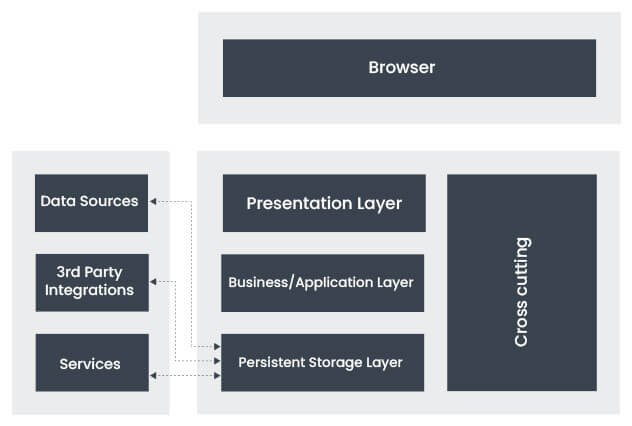
\includegraphics[width=6.10236in,height=4.11111in]{imported-media/media/image9.png}
  \caption[Diagram warstw aplikacji internetowej]{Diagram, przedstawiający warstwy aplikacji internetowej. Źródło: \url{https://www.albiorixtech.com/wp-content/uploads/2025/12/web-application-architecture-layers.jpg} (dostęp: 03.02.2026).}
\end{figure}

Przeglądarka (browser) to środowisko uruchomieniowe po stronie klienta, w którym działa aplikacja frontendowa. Użytkownik korzysta z systemu poprzez przeglądarkę, która renderuje interfejs i wysyła żądania do serwera. Ponadto umożliwia wykonywanie kodu JavaScripta, obsługuje interakcje z systemem, wyświetla interfejs użytkownika oraz może komunikować się z backendem za pomocą protokołów HTTP lub HTTPS\footnote{HTTP (HyperText Transfer Protocol) -- protokół komunikacyjny warstwy aplikacji wykorzystywany do przesyłania danych pomiędzy klientem a serwerem w sieci WWW. Jego rozszerzona, bardziej bezpieczna wersja, wykorzystująca mechanizmy szyfrowania to protokół HTTPS (HyperText Transfer Protocol Secure).}.

Warstwa prezentacji odpowiada za interfejs użytkownika (UI) oraz sposób prezentacji danych. Wyświetla widoki formularzy, zbiera dane wejściowe, które potem mogą zostać przesłane w postaci zapytań do bazy danych oraz zajmuje się podstawową walidacją formularzy. Odpowiada również za wysyłanie zapytań do backendu.

Warstwa logiki biznesowej stanowi rdzeń aplikacji, odpowiadając za przetwarzanie danych. Realizuje operacje CRUD, dbając też o szczegółową walidację danych. Realizuje autentykację i autoryzację użytkowników.

Za magazynowanie danych w sposób trwały odpowiada warstwa przechowywania danych (na rysunku opisana jako persistent storage layer), będąca zazwyczaj bazą danych. Ta część aplikacji odczytuje, przechowywuje i zapewnia integralność danych.

Źródła zewnętrze z kolei to systemy i usługi, z którymi aplikacja się integruje. Mogą to być zewnętrzne bazy lub pliki z danymi (data sources), integracje z systemami firm trzecich (3rd party integrations) lub dodatkowe mikroserwisy oraz API (na schemacie opisane jako services). Mechanizmy przekrojowe (na schemacie, widniejące jako cross-cutting) to elementy, działające na wszystkich warstwach. Nie należą one do konkretnej warstwy, lecz wpływają na cały system. Mogą obejmować na przykład mechanizmy bezpieczeństwa, logowania zdarzeń, obsługę błędów lub monitorowanie wydajności aplikacji.

\section{Diagramy Architektoniczne}

\FirstParagraph Jednym z najważniejszych diagramów, stworzonych podczas procesu projektowania fundamentów aplikacji jest diagram komponentów. Przedstawia on architekturę komponentową aplikacji, zrealizowaną w modelu klient-serwer, z wyraźnym podziałem na interfejs użytkownika (frontend), warstwę API, logikę serwerową (backend), bazę danych oraz zewnętrznych dostawców autentykacji. Strzałki obrazują zależności oraz przepływ danych pomiędzy komponentami.

\begin{figure}[H]
  \centering
  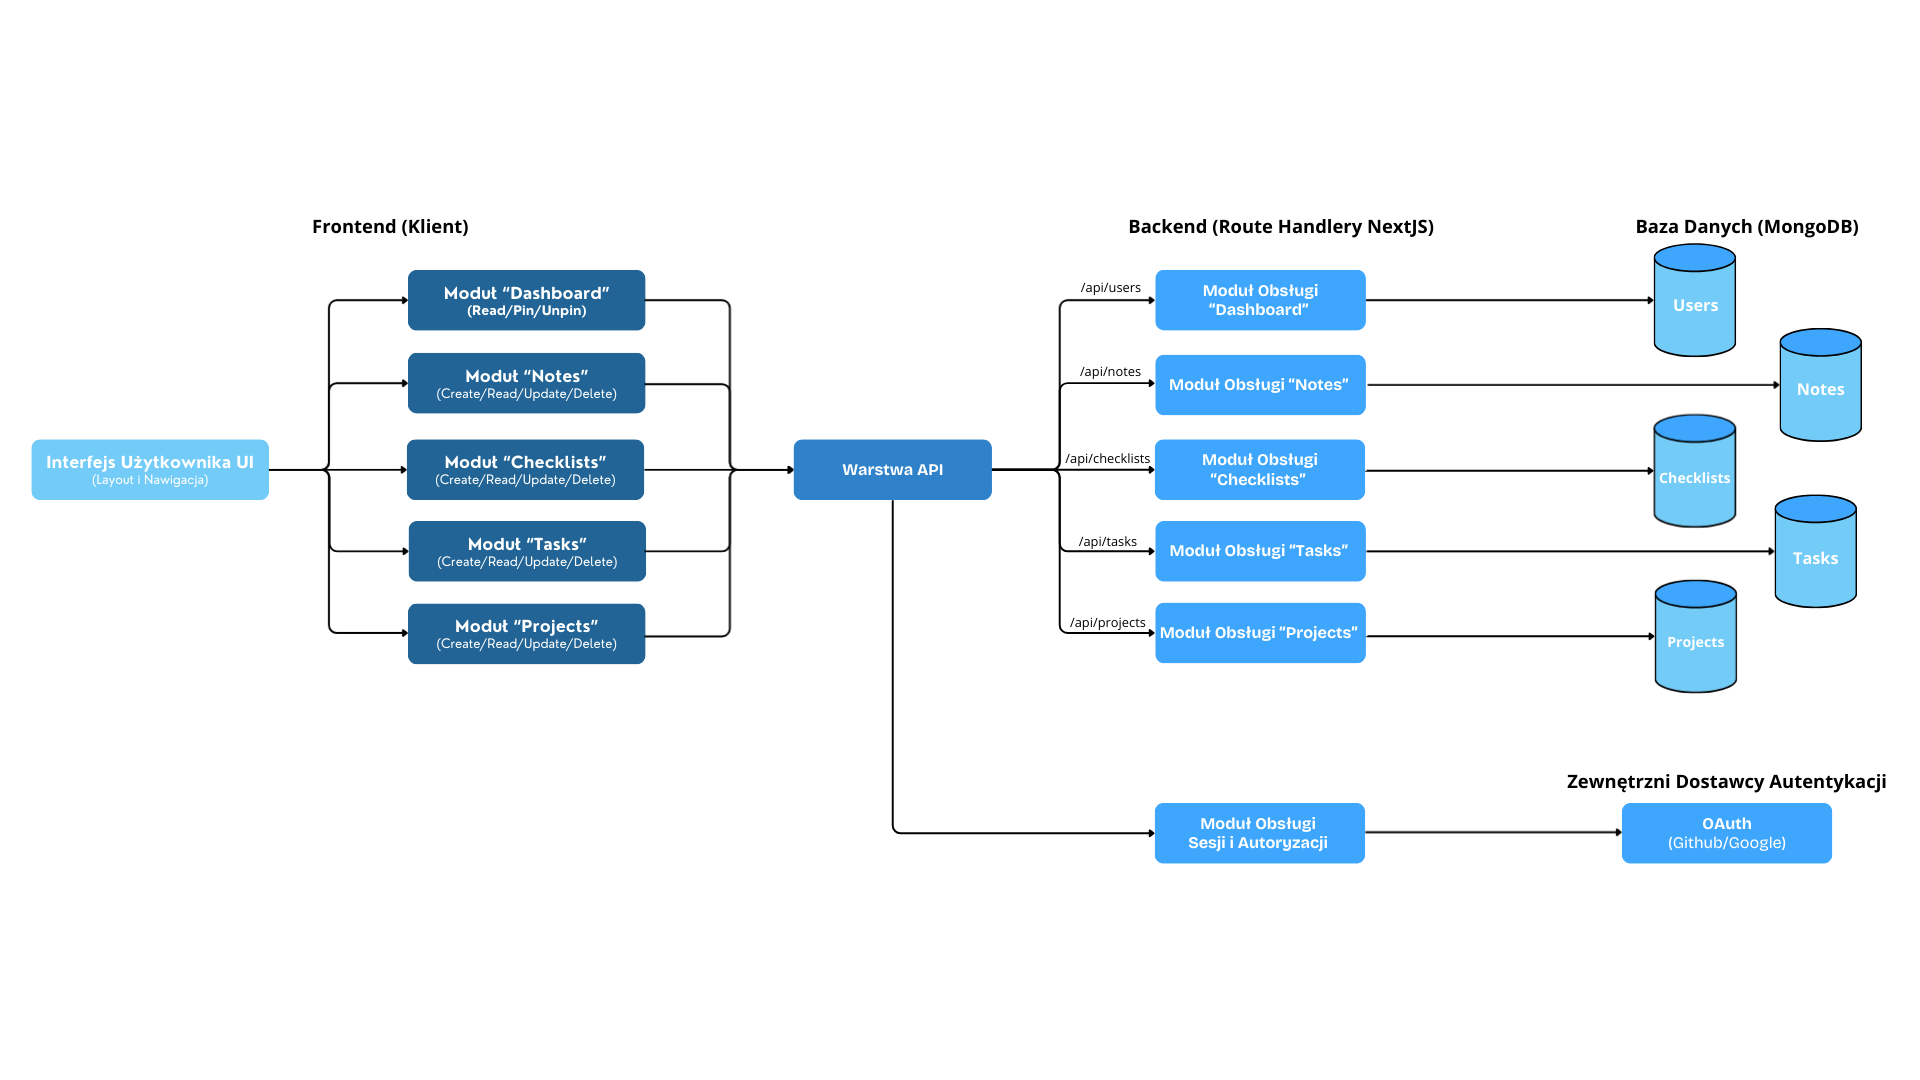
\includegraphics[width=5.53778in,height=3.10511in]{imported-media/media/image10.png}
  \caption{Prosty diagram komponentów internetowej aplikacji do zarządzania zadaniami.}
\end{figure}

Przepływ danych można rozpisać na poszczególne kroki:

\begin{enumerate}
\def\labelenumi{\arabic{enumi}.}
\item
  Użytkownik wykonuje akcję w interfejsie.
\item
  Frontend wysyła żądanie do API.
\item
  Backend przetwarza logikę, sprawdzając również uprawnienia.
\item
  Dane są pobierane lub zapisywane w bazie.
\item
  Odpowiedź wraca do UI.
\end{enumerate}

Najważniejsze idee architektoniczne:

\begin{itemize}
\item
  separacja warstw,
\item
  modularność, wynikająca z osobnych serwisów dla każdego typu zasobu,
\item
  bezpieczeństwo, zapewnione przez brak bezpośredniego dostępu klienta do bazy,
\item
  łatwa skalowalność.
\end{itemize}

Kolejne diagramy, powstałe na etapie projektowania architektury przygotowano, wykorzystując informacje z artykułu ``Canva: DFD''\footnote{Canva, \emph{Creating a data flow diagram: How-tos, templates, and tips}, \url{https://www.canva.com/online-whiteboard/data-flow-diagrams/} (dostęp: 03.02.2026).}. Pokazują jak dane przemieszczają się w systemie między źródłami, procesami oraz magazynami danych. Są to tak zwane jest ``diagramy przepływu danych''.

\begin{figure}[H]
  \centering
  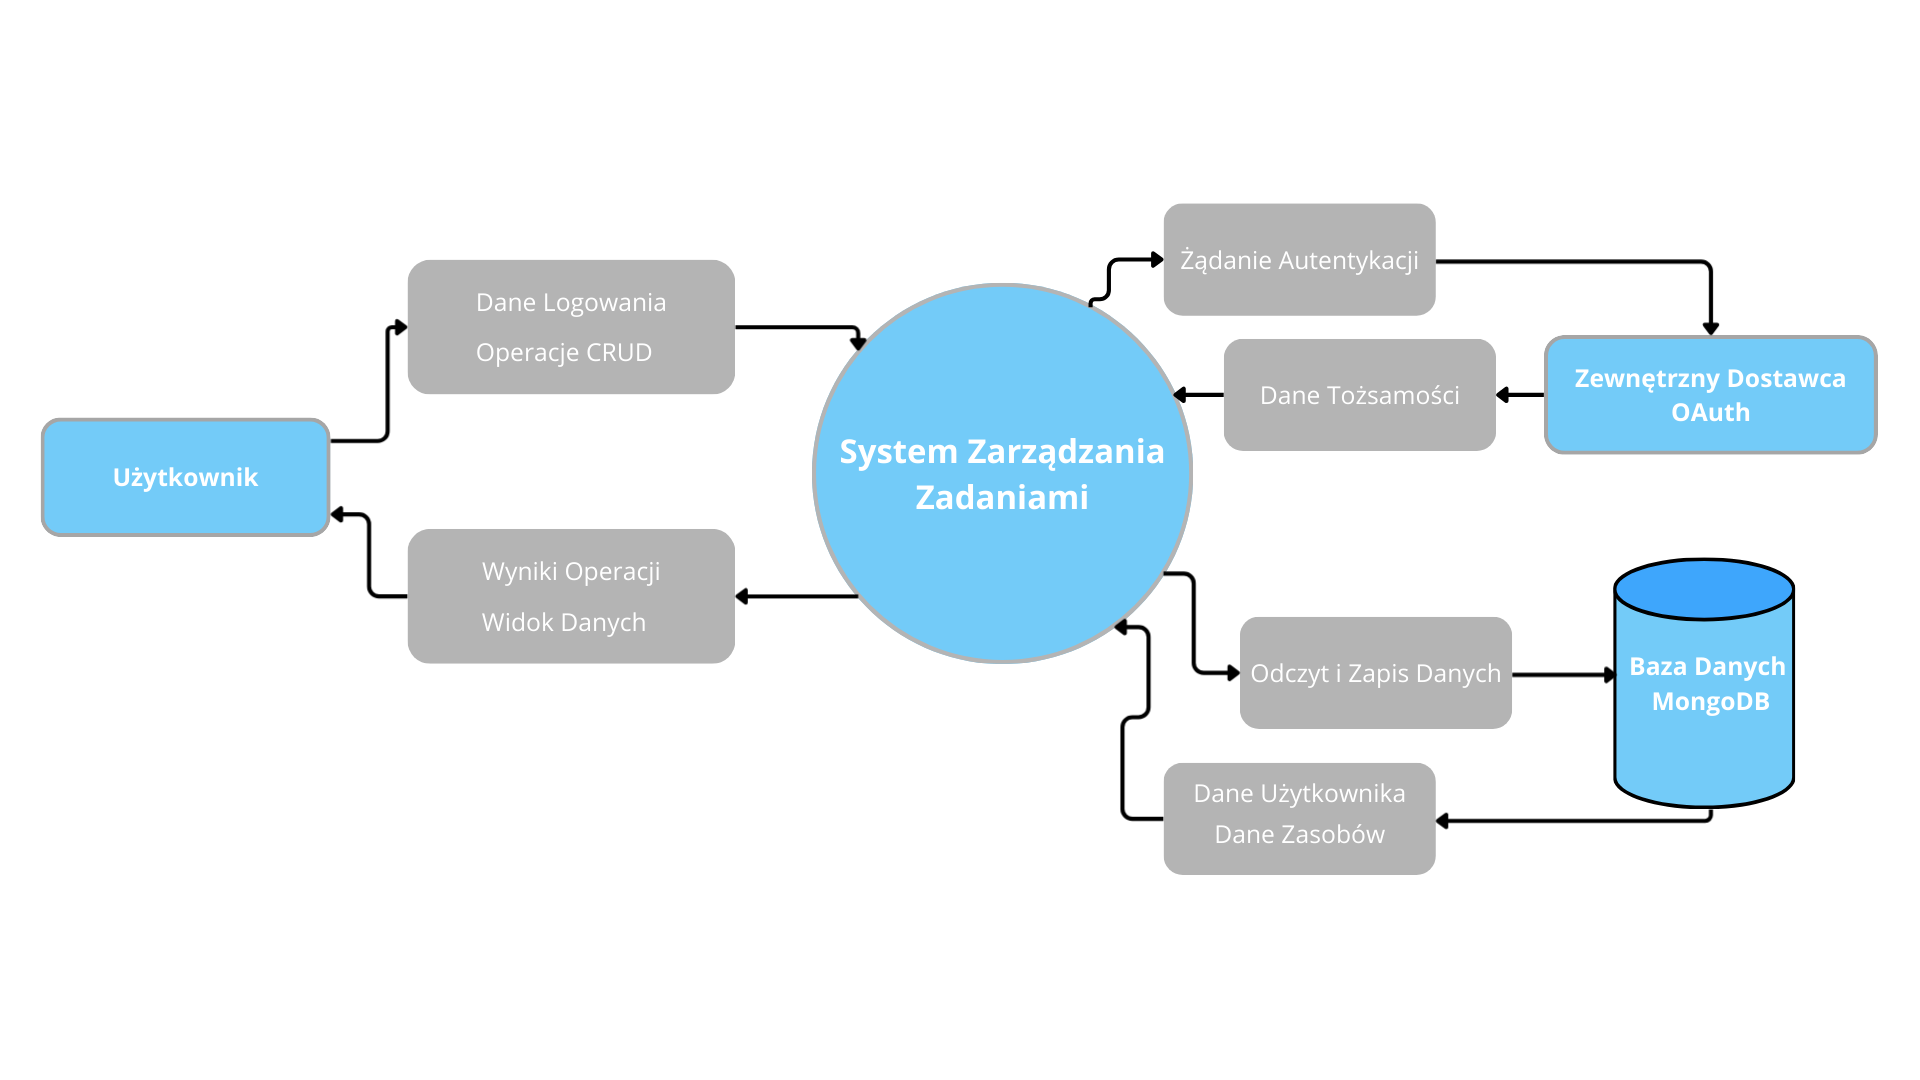
\includegraphics[width=5.53039in,height=3.10322in]{imported-media/media/image11.png}
  \caption{Diagram przepływu danych poziomu 0, przedstawiający system jako jeden proces wraz z relacjami z otoczeniem.}
\end{figure}

Diagram przepływu danych poziomu 0 przedstawia aplikację do zarządzania zadaniami jako pojedynczy, logiczny proces, przetwarzający dane pomiędzy użytkownikiem, zewnętrznym dostawcą autentykacji oraz bazą danych. Użytkownik inicjuje operacje takie jak logowanie oraz zarządzanie zadaniami, projektami, notatkami i checklistami, natomiast system przetwarza te żądania, komunikuje się z bazą danych oraz zwraca odpowiednie wyniki. Diagram ten obrazuje granice systemu oraz jego relacje z otoczeniem, pomijając szczegóły wewnętrznej struktury aplikacji, które przedstawiane są na kolejnym rysunku.

Diagram przepływu danych poziomu 1 przedstawia szczegółową dekompozycję systemu na główne procesy funkcjonalne oraz pokazuje sposób wymiany informacji pomiędzy użytkownikiem, modułami aplikacji, bazą danych i zewnętrznym dostawcą autentykacji. Użytkownik inicjuje operacje takie jak logowanie, przeglądanie oraz zarządzanie zadaniami, projektami, notatkami i checklistami, a odpowiednie procesy systemowe realizują logikę biznesową i wykonują operacje zapisu lub odczytu danych w dedykowanych kolekcjach bazy danych. Dodatkowo wydzielony został proces autentykacji i zarządzania sesją, który komunikuje się z dostawcą OAuth w celu weryfikacji tożsamości użytkownika. Diagram ilustruje rozdzielenie odpowiedzialności pomiędzy warstwą logiki aplikacji i warstwą przechowywania danych.

\begin{figure}[H]
  \centering
  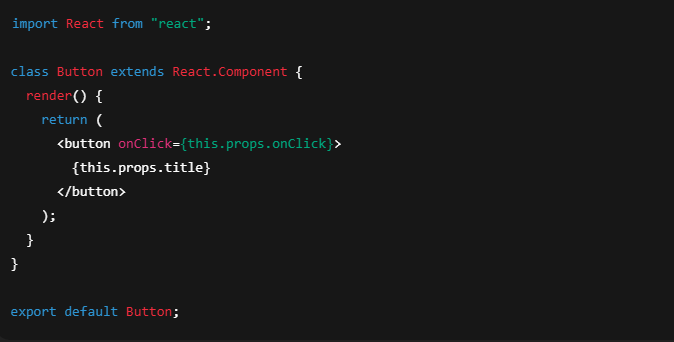
\includegraphics[width=5.47191in,height=4.70023in]{imported-media/media/image12.png}
  \caption{Diagram przepływu danych poziomu 1}
\end{figure}

\section{Struktura bazy danych aplikacji}

\FirstParagraph W aplikacji zastosowano bazę danych MongoDB oraz bibliotekę Mongoose, która została wykorzystana do opisania struktury dokumentów domenowych. Połączenie z bazą jest realizowane przez moduł odpowiedzialny za utrzymywanie współdzielonego połączenia Mongoose, natomiast mechanizm logowania OAuth korzysta dodatkowo z adaptera MongoDB dla NextAuth. Dzięki temu dane logowania oraz dane aplikacyjne są przechowywane w tej samej bazie, ale obsługiwane przez odrębne warstwy aplikacji.

Podstawową zasadą modelu danych jest przypisanie dokumentów do konkretnego użytkownika. Notatki, checklisty, zadania, projekty, przypięcia oraz zdarzenia aktywności zawierają pole ``\texttt{ownerId}'', które wskazuje właściciela dokumentu. Preferencje interfejsu użytkownika korzystają z pola ``\texttt{userId}''. Każda operacja pobierania, aktualizacji lub archiwizacji danych wykonywana jest z uwzględnieniem identyfikatora aktualnie zalogowanego użytkownika, co zabezpiecza aplikację przed dostępem do cudzych zasobów.

\begin{figure}[H]
  \centering
  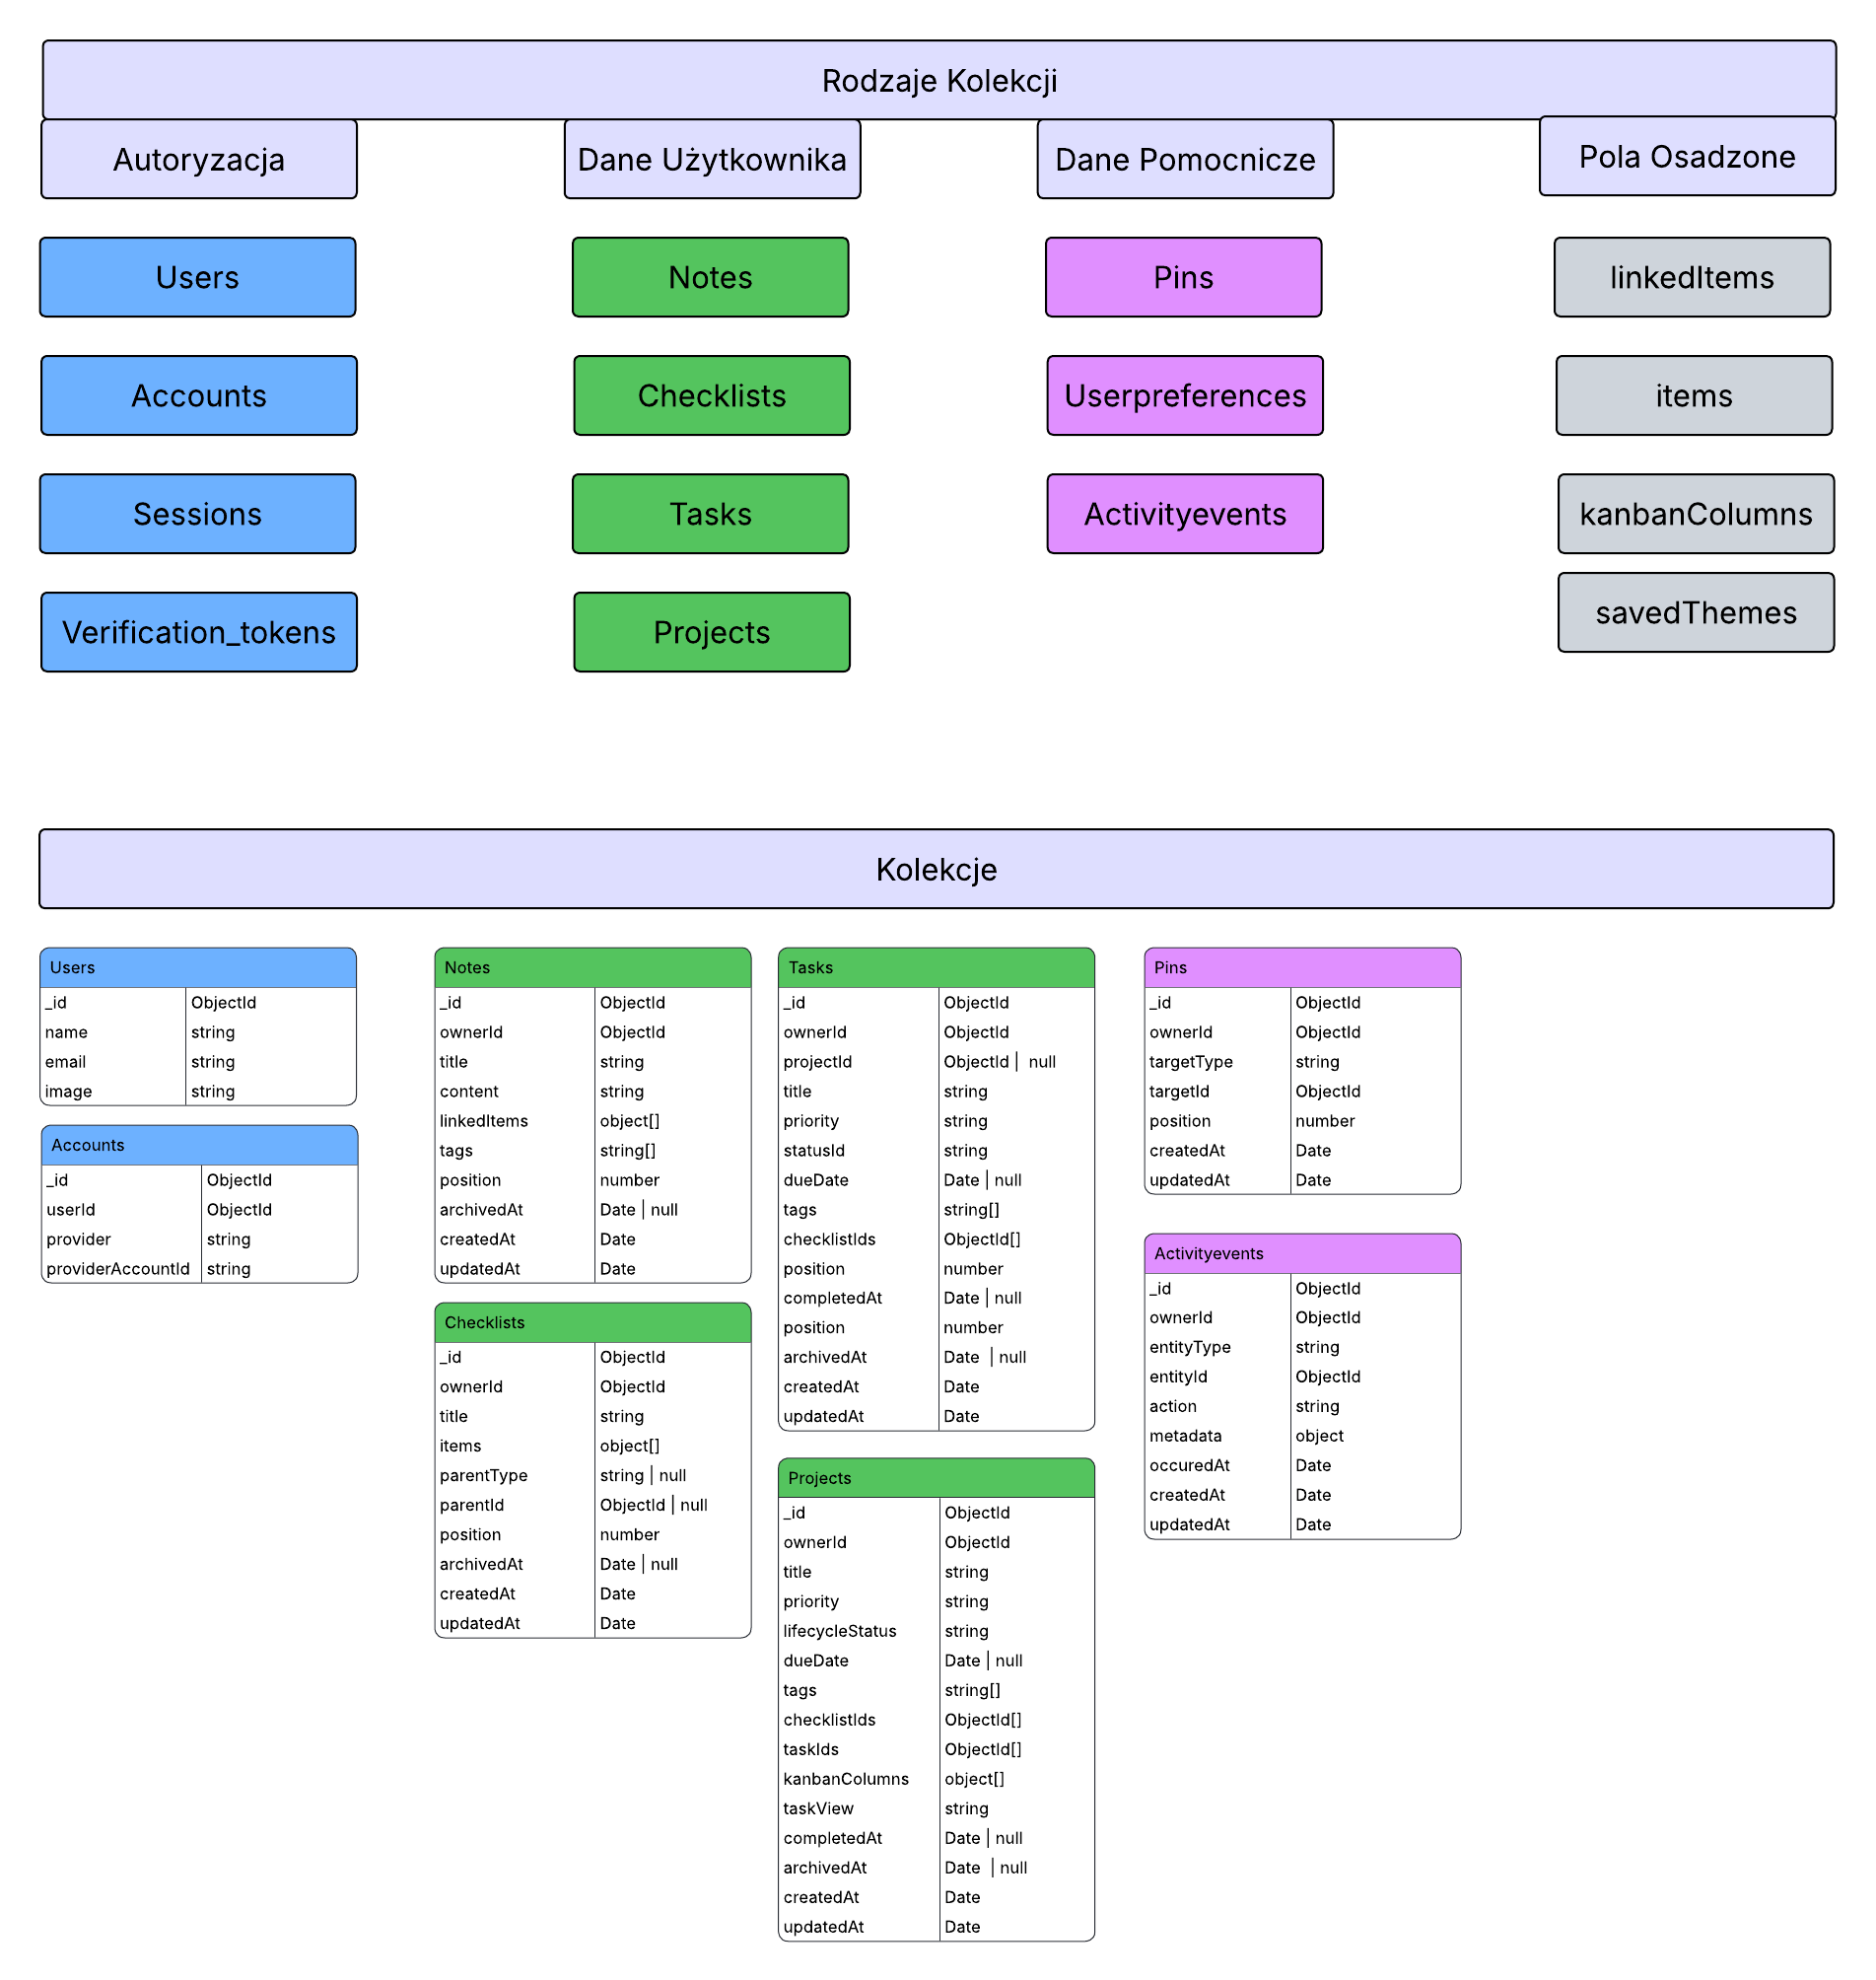
\includegraphics[width=\textwidth,height=0.82\textheight,keepaspectratio]{assets/schemat-bazy-danych.png}
  \caption{Schemat struktury bazy danych aplikacji.}
  \label{fig:schemat-bazy-danych-aplikacji}
\end{figure}

Na rysunku powyżej przedstawiono graficzny schemat struktury bazy danych aplikacji. Diagram został podzielony na cztery grupy: kolekcje autoryzacyjne, kolekcje przechowujące dane użytkownika, kolekcje pomocnicze oraz pola osadzone. Taki podział pokazuje, że dane odpowiedzialne za logowanie użytkownika są odseparowane od danych domenowych aplikacji, takich jak zadania, projekty, checklisty i notatki.

W schemacie zastosowano oznaczenie ``\texttt{ObjectId}'', które oznacza specjalny typ identyfikatora używany w MongoDB. Każdy dokument zapisany w kolekcji otrzymuje pole ``\texttt{\_id}'' tego typu, a inne pola, takie jak ``\texttt{ownerId}'', ``\texttt{projectId}'', ``\texttt{targetId}'' albo ``\texttt{userId}'', mogą przechowywać identyfikator innego dokumentu. Dzięki temu aplikacja może wskazywać powiązania pomiędzy dokumentami bez stosowania klasycznych kluczy obcych znanych z relacyjnych baz danych.

Typ ``\texttt{Date}'' zapisany jest wielką literą, ponieważ w kontekście MongoDB, Mongoose oraz JavaScriptu jest to nazwa typu obiektowego reprezentującego datę i czas. Zapis ma więc charakter techniczny i odpowiada nazwie typu, a nie zwykłemu słowu opisowemu. Z tego samego powodu na diagramie widoczne są zapisy takie jak ``\texttt{Date | null}'', które oznaczają, że pole może zawierać datę albo wartość pustą. Przykładem jest ``\texttt{archivedAt}'', które pozostaje puste dla aktywnego dokumentu, a po archiwizacji otrzymuje datę wykonania tej operacji.

Zapisy z nawiasami kwadratowymi, takie jak ``\texttt{string[]}'', ``\texttt{ObjectId[]}'' albo ``\texttt{object[]}'', oznaczają tablice wartości danego typu. Przykładowo ``\texttt{string[]}'' oznacza tablicę tekstów, czyli wiele wartości typu ``\texttt{string}''. Pole ``\texttt{tags}'' może więc przechowywać kilka tagów, pole ``\texttt{checklistIds}'' może przechowywać wiele identyfikatorów checklist, a pole ``\texttt{kanbanColumns}'' zawiera tablicę obiektów opisujących kolumny tablicy kanban.

Warstwa autoryzacji tworzy cztery kolekcje. Są to ``\texttt{users}'', ``\texttt{accounts}'', ``\texttt{sessions}'' oraz ``\texttt{verification\_tokens}''. Najważniejsze z punktu widzenia działania aplikacji są kolekcje ``\texttt{users}'' i ``\texttt{accounts}'', ponieważ przechowują użytkowników oraz powiązania z zewnętrznymi dostawcami logowania, takimi jak Google i GitHub. Sesja użytkownika jest obsługiwana z użyciem strategii JWT, jednak identyfikator użytkownika pochodzący z NextAuth stanowi podstawę powiązań z dokumentami domenowymi.

Kolekcja ``\texttt{accounts}'' pełni funkcję technicznego powiązania pomiędzy użytkownikiem zapisanym w kolekcji ``\texttt{users}'' a kontem pochodzącym od zewnętrznego dostawcy logowania. Pole ``\texttt{userId}'' wskazuje dokument użytkownika, natomiast pola ``\texttt{provider}'' i ``\texttt{providerAccountId}'' określają, z jakiego dostawcy OAuth pochodzi dane konto oraz jaki identyfikator użytkownik posiada u tego dostawcy. Dzięki temu jedna osoba może być poprawnie rozpoznawana przez system po zalogowaniu z użyciem zewnętrznej usługi.

Główne dane aplikacji zostały podzielone na kolekcje ``\texttt{notes}'', ``\texttt{checklists}'', ``\texttt{tasks}'', ``\texttt{projects}'', ``\texttt{pins}'', ``\texttt{userpreferences}'' oraz ``\texttt{activityevents}''. Kolekcja ``\texttt{notes}'' przechowuje notatki użytkownika, zawierające tytuł, treść, tagi, pozycję sortowania oraz listę powiązanych elementów. Powiązania notatki są przechowywane w tablicy ``\texttt{linkedItems}'', gdzie każdy wpis składa się z typu obiektu oraz jego identyfikatora. Dzięki temu notatka może odnosić się do innej notatki, checklisty, zadania albo projektu.

Checklisty są przechowywane w kolekcji ``\texttt{checklists}''. Każda checklista posiada tytuł, pozycję, opcjonalne powiązanie z rodzicem oraz tablicę elementów. Elementy checklisty zostały osadzone bezpośrednio w dokumencie checklisty, ponieważ są odczytywane i aktualizowane razem z nią. Pojedynczy element zawiera nazwę, informację o ukończeniu, datę ukończenia oraz pozycję. Checklista może funkcjonować samodzielnie albo być powiązana z zadaniem lub projektem przez pola ``\texttt{parentType}'' i ``\texttt{parentId}''.

Zadania są zapisywane w kolekcji ``\texttt{tasks}''. Dokument zadania zawiera tytuł, opis, priorytet, status, termin wykonania, tagi, pozycję, datę ukończenia oraz datę archiwizacji. Zadanie może być samodzielnym elementem listy zadań albo częścią projektu. W drugim przypadku pole ``\texttt{projectId}'' wskazuje projekt, do którego należy zadanie. Status zadania jest przechowywany w polu ``\texttt{statusId}''; w widoku tablicy kanban odpowiada on identyfikatorowi jednej z kolumn projektu. Zadanie może mieć również powiązane checklisty, których identyfikatory są przechowywane w tablicy ``\texttt{checklistIds}''.

Projekty są przechowywane w kolekcji ``\texttt{projects}''. Dokument projektu zawiera tytuł, opis, priorytet, status cyklu życia, termin, tagi, pozycję, listę zadań, checklisty oraz konfigurację widoku zadań. W projekcie przechowywana jest tablica ``\texttt{kanbanColumns}'', opisująca kolumny tablicy kanban. Każda kolumna ma identyfikator, nazwę, kolor, pozycję oraz informację, czy oznacza stan zakończony. Domyślny zestaw kolumn obejmuje ``\texttt{backlog}'', ``\texttt{todo}'', ``\texttt{in\_progress}'', ``\texttt{testing}'' oraz ``\texttt{done}''. Pole ``\texttt{taskView}'' określa, czy zadania projektu są prezentowane jako lista, czy jako tablica kanban. 

Relacja pomiędzy projektami i zadaniami jest utrzymywana dwukierunkowo na poziomie aplikacji. Główne powiązanie znajduje się w zadaniu, w polu ``\texttt{projectId}''. Projekt przechowuje dodatkowo tablicę ``\texttt{taskIds}'', która zawiera identyfikatory powiązanych zadań. Podczas tworzenia zadania z przypisanym projektem backend sprawdza, czy projekt istnieje, nie jest zarchiwizowany i należy do aktualnego użytkownika. Następnie identyfikator zadania jest dopisywany do projektu. Przy zmianie projektu lub archiwizacji zadania identyfikator jest usuwany ze starego projektu.

Kolekcja ``\texttt{pins}'' przechowuje elementy przypięte na ekranie głównym aplikacji. Dokument przypięcia zawiera typ wskazywanego obiektu, jego identyfikator oraz pozycję na dashboardzie. Dzięki parze pól ``\texttt{targetType}'' i ``\texttt{targetId}'' możliwe jest przypięcie notatki, checklisty, zadania albo projektu bez tworzenia osobnych kolekcji dla każdego typu przypięcia. W modelu zastosowano unikalny indeks obejmujący właściciela, typ celu i identyfikator celu, co zapobiega wielokrotnemu przypięciu tego samego elementu przez jednego użytkownika.

Na schemacie kolekcja ``\texttt{pins}'' została umieszczona w grupie danych pomocniczych, ponieważ sama nie przechowuje pełnej treści notatki, taska, checklisty ani projektu. Jest dokumentem pośrednim, który zapamiętuje, jaki element użytkownik chce widzieć na dashboardzie. Pole ``\texttt{targetType}'' określa typ przypiętego obiektu, a ``\texttt{targetId}'' przechowuje jego identyfikator. Taki układ upraszcza model danych, ponieważ jeden mechanizm przypinania obsługuje kilka typów zasobów.

Preferencje interfejsu zapisano w kolekcji ``\texttt{userpreferences}''. Dokument preferencji zawiera tryb kolorystyczny, układ dashboardu, zestaw kolorów używanych w aplikacji oraz zapisane własne motywy. Pole ``\texttt{userId}'' jest unikalne, dlatego jeden użytkownik ma jeden dokument preferencji. Takie rozwiązanie upraszcza pobieranie ustawień podczas renderowania interfejsu.

Kolekcja ``\texttt{activityevents}'' przechowuje zdarzenia aktywności. Zdarzenie zawiera typ encji, identyfikator dokumentu, rodzaj akcji oraz czas wystąpienia. Rejestrowane są między innymi operacje utworzenia, aktualizacji, usunięcia, przeniesienia oraz przypięcia elementu. Endpoint odpowiedzialny za komunikację w czasie rzeczywistym odczytuje te zdarzenia i przekazuje je klientowi za pomocą mechanizmu SSE, co pozwala odświeżać widoki po zmianach danych.

Najważniejsze relacje logiczne w bazie danych można przedstawić następująco:

\begin{itemize}
\item
  użytkownik jest właścicielem notatek, checklist, zadań, projektów, przypięć i zdarzeń aktywności,
\item
  użytkownik posiada jeden dokument preferencji interfejsu,
\item
  zadanie może należeć do projektu przez pole ``\texttt{projectId}'',
\item
  projekt przechowuje pomocniczą listę zadań w tablicy ``\texttt{taskIds}'',
\item
  zadanie i projekt mogą mieć powiązane checklisty,
\item
  notatka może wskazywać inne elementy aplikacji przez tablicę ``\texttt{linkedItems}'',
\item
  przypięcie wskazuje dowolny obsługiwany typ elementu przez pola ``\texttt{targetType}'' i ``\texttt{targetId}''.
\end{itemize}

W bazie zastosowano indeksy wspierające najczęstsze operacje aplikacji. Większość kolekcji posiada indeksowanie po polu właściciela, co przyspiesza pobieranie danych aktualnego użytkownika. Dodatkowe indeksy obejmują między innymi pozycję sortowania, tagi, termin wykonania, priorytet, status zadania oraz pola wykorzystywane do przypięć. Dzięki temu aplikacja może sprawnie filtrować zadania i projekty, sortować elementy dashboardu oraz szybko sprawdzać, czy dany element został już przypięty.

Usuwanie większości elementów domenowych zostało zrealizowane jako archiwizacja. Zadania, projekty i checklisty otrzymują wartość w polu ``\texttt{archivedAt}'', a zapytania listujące pobierają wyłącznie dokumenty aktywne. W przypadku projektu podczas archiwizacji ustawiany jest również status cyklu życia ``\texttt{archived}''. Takie podejście pozwala zachować spójność powiązań i historię zmian bez fizycznego usuwania dokumentów.

\chapter{Projekt interfejsu użytkownika}

\FirstParagraph Projekt interfejsu użytkownika, jest jednym z najważniejszych aspektów aplikacji. Przejrzystość, czytelność oraz prostota obsługi decydują w dużej mierze o użyteczności. W tym celu najpierw rozpisane zostały historie użytkownika, po których analizie powstał graficzny projekt interfejsu.

\section{Scenariusze przypadków użycia}

\FirstParagraph \textbf{1) Przypięcie elementu do strony głównej}

\textbf{Aktor:} Użytkownik indywidualny

\textbf{Cel:} Szybki dostęp do śledzonych tasków/notatek/checklist/projektów z poziomu strony głównej

\textbf{Warunki wstępne:} Użytkownik jest zalogowany; Element istnieje

\textbf{Scenariusz podstawowy:}

\begin{enumerate}
\def\labelenumi{\arabic{enumi}.}
\item
  Użytkownik otwiera którąś z list elementów (taski/checklisty/projekty itd.)
\item
  Użytkownik wybiera konkretny element
\item
  Użytkownik widzi, że element nie jest przypięty(ikonka pinezki pusta w środku)
\item
  Użytkownik klika na ikonkę i dodaje do przypiętych
\item
  System oznacza element jako „przypięty'' poprzez zmianę ikonki pinezki na wypełnioną
\item
  System wyświetla element w sekcji ``przypięte'' na stronie głównej.
\end{enumerate}

\textbf{Scenariusze alternatywne / wyjątki:}

\begin{enumerate}
\def\labelenumi{\arabic{enumi}.}
\item
  \textbf{Element już jest przypięty}\\
  3a. System daje użytkownikowi informację, że element jest już przypięty poprzez (wypełnioną ikonę pinezki)\\
  4a. Użytkownik może kliknąć ikonkę w celu odpięcia elementu od ekranu głównego.
\end{enumerate}

\textbf{Warunki końcowe:} Element jest widoczny w sekcji „przypięte'' na stronie głównej

\vspace{\baselineskip}

\textbf{2) Utworzenie nowego zadania z parametrami}

\textbf{Aktor:} Pracownik biurowy

\textbf{Cel:} Uporządkowanie pracy poprzez utworzenie zadania z właściwościami

\textbf{Warunki wstępne:} Użytkownik jest zalogowany

\textbf{Scenariusz podstawowy:}

\begin{enumerate}
\def\labelenumi{\arabic{enumi}.}
\item
  Użytkownik wybiera z paska bocznego zakładkę ``zadania''
\item
  Użytkownik zostaje przekierowany na stronę z zadaniami
\item
  Użytkownik wybiera ikonkę z plusem, znajdującą się obok istniejących zadań
\item
  System otwiera formularz tworzenia zadania
\item
  Użytkownik wpisuje nazwę zadania
\item
  Użytkownik uzupełnia opis zadania
\item
  Użytkownik wybiera priorytet z rozwijanej listy wyboru
\item
  Użytkownik ustawia datę realizacji zadania
\item
  Użytkownik zapisuje zadanie
\item
  System tworzy zadanie i wyświetla je w liście zadań na stronie
\end{enumerate}

\textbf{Scenariusze alternatywne / wyjątki:}

\begin{enumerate}
\def\labelenumi{\arabic{enumi}.}
\item
  \textbf{Brak opisu}\\
  6a. Użytkownik pomija opis; system zapisuje zadanie bez opisu.
\item
  \textbf{Brak wymaganych danych (np. nazwy)}\\
  5a. Użytkownik pomija nazwę zadania.\\
  9a. System blokuje zapis i wskazuje brakujące pola.
\item
  \textbf{Niepoprawna data realizacji}\\
  8a. Użytkownik ustawia datę z przeszłości.\\
  9a. System blokuje zapis i wskazuje błędną datę.
\end{enumerate}

\textbf{Warunki końcowe:} Dodane zadanie wraz z opisem, priorytetem i datą realizacji pojawiają się w liście zadań

\begin{figure}[H]
  \centering
  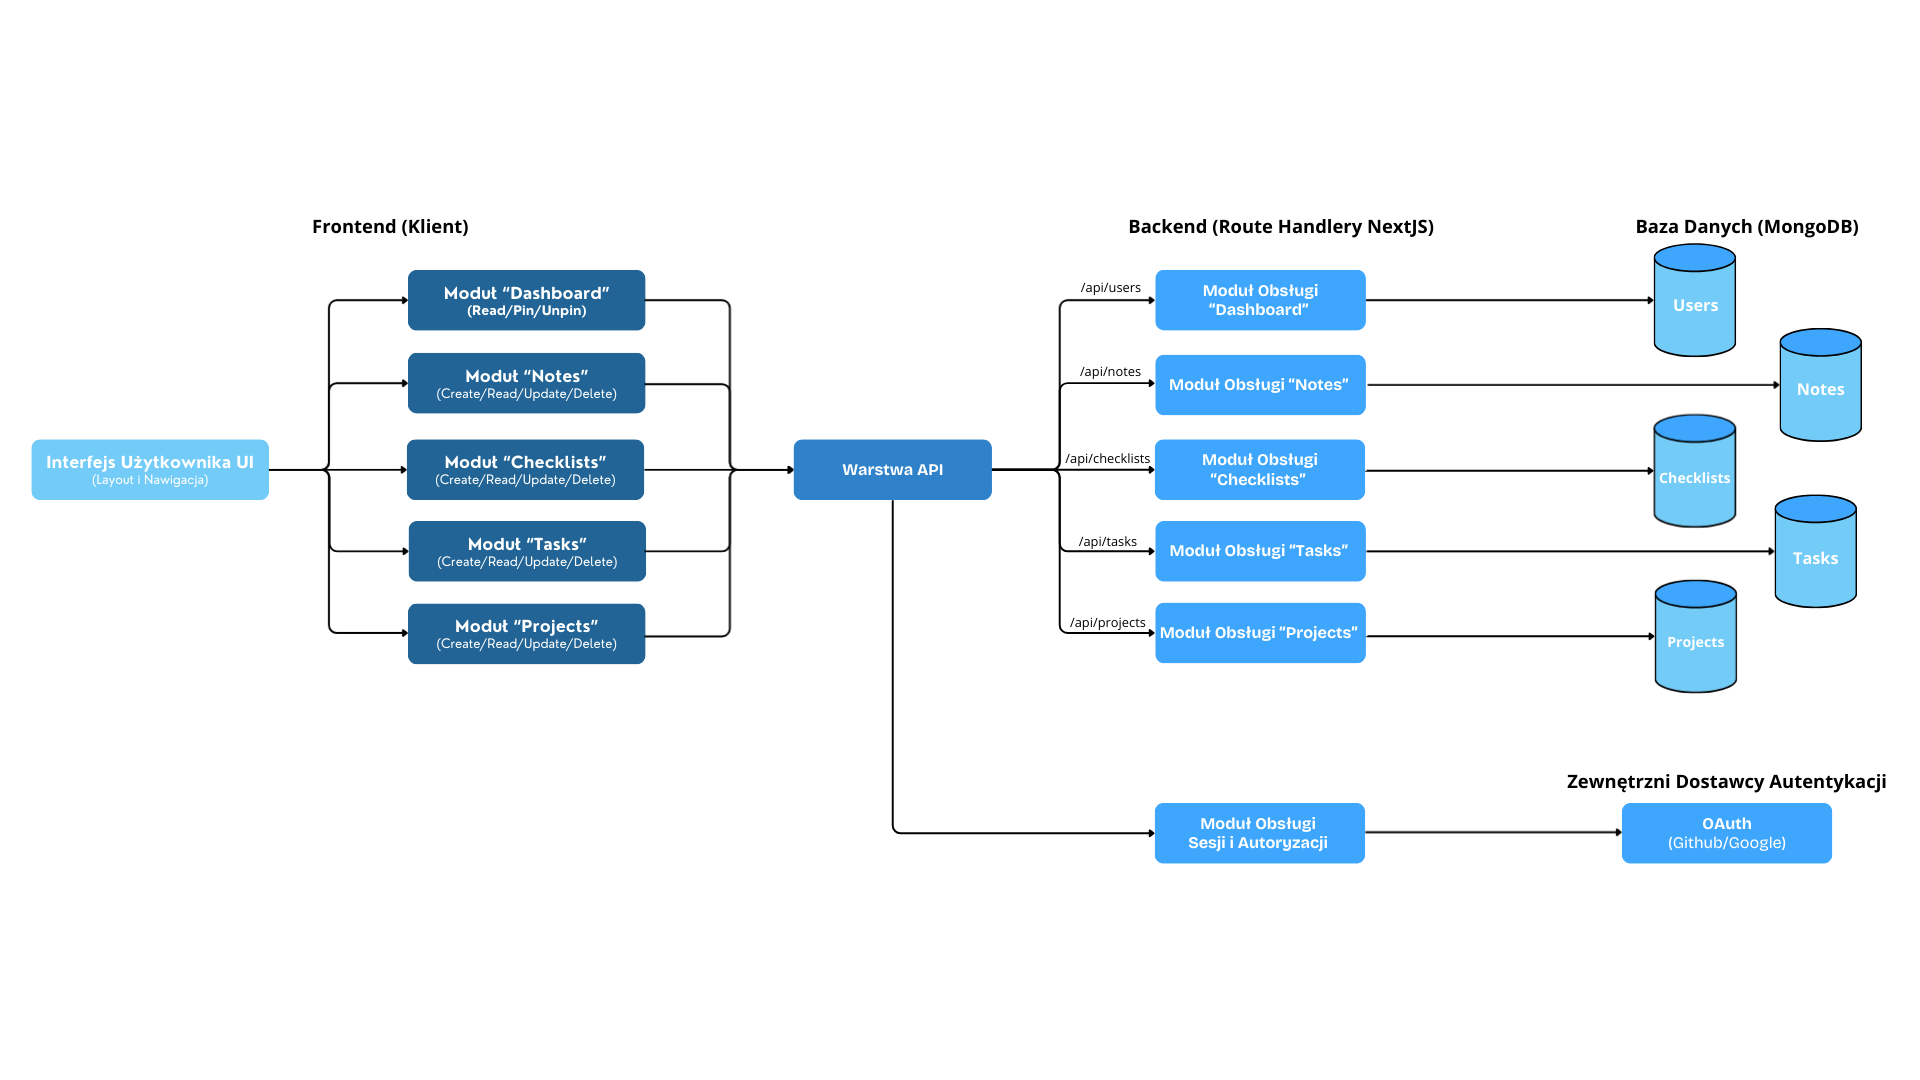
\includegraphics[width=4.9in]{imported-media/media/image13.png}
  \caption{Diagram UML, wizualizujący scenariusz przypięcia taska}
\end{figure}

Na diagramie zaprezentowano sekwencję działań wykonywanych podczas przypinania taska do strony głównej aplikacji. Widoczny jest podział odpowiedzialności pomiędzy użytkownika, interfejs aplikacji oraz system zapisujący zmianę. Po wybraniu elementu użytkownik otrzymuje informację o aktualnym stanie przypięcia, a następnie może zmienić ten stan za pomocą ikony pinezki.

\vspace{\baselineskip}

\textbf{3) Utworzenie checklisty zakupów z możliwością odhaczanie pozycji}

\textbf{Aktor:} Głowa rodziny

\textbf{Cel:} Nie zapomnieć produktów w sklepie

\textbf{Warunki wstępne:} Użytkownik jest zalogowany

\textbf{Scenariusz podstawowy:}

\begin{enumerate}
\def\labelenumi{\arabic{enumi}.}
\item
  Użytkownik przechodzi do strony ``szybkie notatki''
\item
  Użytkownik wybiera ikonkę z plusem, znajdującą się obok istniejących elementów
\item
  Użytkownik wybiera czy chce dodać notatkę, czy checklistę
\item
  System otwiera formularz tworzenia checklisty
\item
  Użytkownik ustawia nazwę checklisty
\item
  Użytkownik dodaje pozycje w checkliście (np. mleko, chleb, warzywa)
\item
  System zapisuje checklistę i wyświetla ją użytkownikowi.
\item
  W sklepie użytkownik otwiera checklistę
\item
  Użytkownik odhacza kolejne pozycje
\item
  System zapisuje, które przedmioty w checkliście zostały odhaczone
\end{enumerate}

\textbf{Scenariusze alternatywne / wyjątki:}

\begin{enumerate}
\def\labelenumi{\arabic{enumi}.}
\item
  \textbf{Dodanie pozycji w trakcie zakupów}\\
  7a. Użytkownik dodaje nową pozycję.\\
  8a. System aktualizuje checklistę.
\end{enumerate}

\textbf{Warunki końcowe:} Checklista zakupów istnieje, a pozycje mogą być odhaczane i zapisywane.

\vspace{\baselineskip}

\textbf{4) Tworzenie notatki}

\textbf{Aktor:} Pracownik nadzorujący dostawy w restauracji

\textbf{Cel:} Utworzenie notatki zawierającej informacje o przebiegu dostawy oraz liczbie palet zwróconych przez restaurację.

\textbf{Warunki wstępne:} Użytkownik jest zalogowany w systemie; użytkownik ma dostęp do sekcji notatek.

\textbf{Scenariusz podstawowy:}

\begin{enumerate}
\def\labelenumi{\arabic{enumi}.}
\item
  Użytkownik przechodzi do strony z notatkami.
\item
  System wyświetla listę istniejących notatek.
\item
  Użytkownik wybiera przycisk dodania nowej notatki.
\item
  System otwiera formularz tworzenia notatki.
\item
  Użytkownik wpisuje tytuł notatki, np. „Dostawa - restauracja''.
\item
  Użytkownik wpisuje treść notatki, zawierającą informacje o przebiegu dostawy.
\item
  Użytkownik dopisuje informację o liczbie palet zwróconych przez restaurację.
\item
  Użytkownik opcjonalnie dodaje tagi porządkujące notatkę, np. „dostawa'' lub „restauracja''.
\item
  Użytkownik zapisuje notatkę.
\item
  System tworzy notatkę i zapisuje ją w bazie danych.
\item
  System wyświetla utworzoną notatkę na liście notatek.
\end{enumerate}

\textbf{Scenariusze alternatywne / wyjątki:}

\begin{enumerate}
\def\labelenumi{\arabic{enumi}.}
\item
  \textbf{Brak treści notatki}\\
  6a. Użytkownik pomija wpisanie treści notatki.\\
  9a. System zapisuje notatkę z samym tytułem.
\item
  \textbf{Brak wymaganej nazwy notatki}\\
  5a. Użytkownik nie wpisuje tytułu notatki.\\
  9a. System blokuje zapis i informuje użytkownika o konieczności podania tytułu.
\item
  \textbf{Dodanie powiązania z innym elementem}\\
  8a. Użytkownik wybiera element aplikacji, z którym notatka ma zostać powiązana, np. task, projekt lub checklistę.\\
  9a. System zapisuje notatkę wraz z informacją o powiązanym elemencie.
\item
  \textbf{Anulowanie tworzenia notatki}\\
  4a. System wyświetla formularz tworzenia notatki.\\
  5a. Użytkownik rezygnuje z dodawania notatki i wraca do listy notatek.\\
  6a. System nie zapisuje żadnych danych i ponownie wyświetla listę notatek.
\end{enumerate}

\textbf{Warunki końcowe:} Notatka zostaje utworzona i jest widoczna na liście notatek. Użytkownik może później otworzyć jej podgląd, edytować treść, dodać tagi lub powiązać ją z innymi elementami aplikacji.

\vspace{\baselineskip}

\textbf{5) Utworzenie projektu i zarządzanie podzadaniami w widoku tablicy}

\textbf{Aktor:} Student

\textbf{Cel:} Organizacja pisania pracy dyplomowej poprzez projekt i podzadania

\textbf{Warunki wstępne:} Użytkownik zalogowany

\textbf{Scenariusz podstawowy:}

\begin{enumerate}
\def\labelenumi{\arabic{enumi}.}
\item
  Użytkownik przechodzi do strony z projektami
\item
  Użytkownik wybiera ikonkę z plusem, znajdującą się obok istniejących projektów
\item
  System Otwiera formularz kreacji projektu
\item
  Użytkownik ustawia nazwę projektu
\item
  Użytkownik ustawia datę realizacji projektu
\item
  Użytkownik dodaje opis projektu
\item
  Użytkownik chce dodać taski do projektu
\item
  System otwiera użytkownikowi formularz dodawania tasków
\item
  Użytkownik może wybrać - czy dodać istniejący już task, czy stworzyć nowy
\item
  Użytkownik dodaje kilka tasków do projektu
\item
  Użytkownik ustawia statusy poszczególnym zadaniom
\item
  Użytkownik zapisuje projekt
\item
  Użytkownik uruchamia stronę projektu i przegląda jego opis
\item
  Użytkownik przełącza widok tasków z listy na tablicę
\item
  System wyświetla kolumny statusów oraz karty podzadań.
\item
  Użytkownik przeciąga karty między kolumnami, zmieniając w ten sposób ich status
\item
  System zapisuje zmiany statusów.
\end{enumerate}

\textbf{Scenariusze alternatywne / wyjątki:}

\begin{enumerate}
\def\labelenumi{\arabic{enumi}.}
\item
  \textbf{Brak daty realizacji}\\
  6a. Użytkownik pomija wypełnianie daty realizacji.\\
  12a. System zapisuje projekt bez daty realizacji.
\item
  \textbf{Brak wymaganych danych (np. nazwy)}\\
  4a. Użytkownik pomija nazwę projektu.\\
  12a. System blokuje zapis i wskazuje brakujące pola.
\item
  \textbf{Niepoprawna data realizacji}\\
  5a. Użytkownik ustawia datę z przeszłości.\\
  12a. System blokuje zapis i wskazuje błędną datę.
\end{enumerate}

\textbf{Warunki końcowe:} Projekt istnieje z opisem, datą i innymi wypełnionymi parametrami a system może wyświetlać taski zarówno w formie listy jak i tablicy

\section{Widoki użytkownika aplikacji}

\FirstParagraph W niniejszym podrozdziale przedstawiono wybrane widoki aplikacji, które odpowiadają scenariuszom przypadków użycia opisanym w poprzedniej części rozdziału. Zaprezentowane ekrany dotyczą przypięcia checklisty do strony głównej, utworzenia taska oraz utworzenia projektu z taskami wyświetlanymi w widoku tablicy kanban i w widoku listy. Opis koncentruje się na układzie interfejsu graficznego, sposobie prezentacji danych oraz elementach ułatwiających użytkownikowi rozpoznanie aktualnego stanu wykonywanych czynności.

\begin{figure}[H]
  \centering
  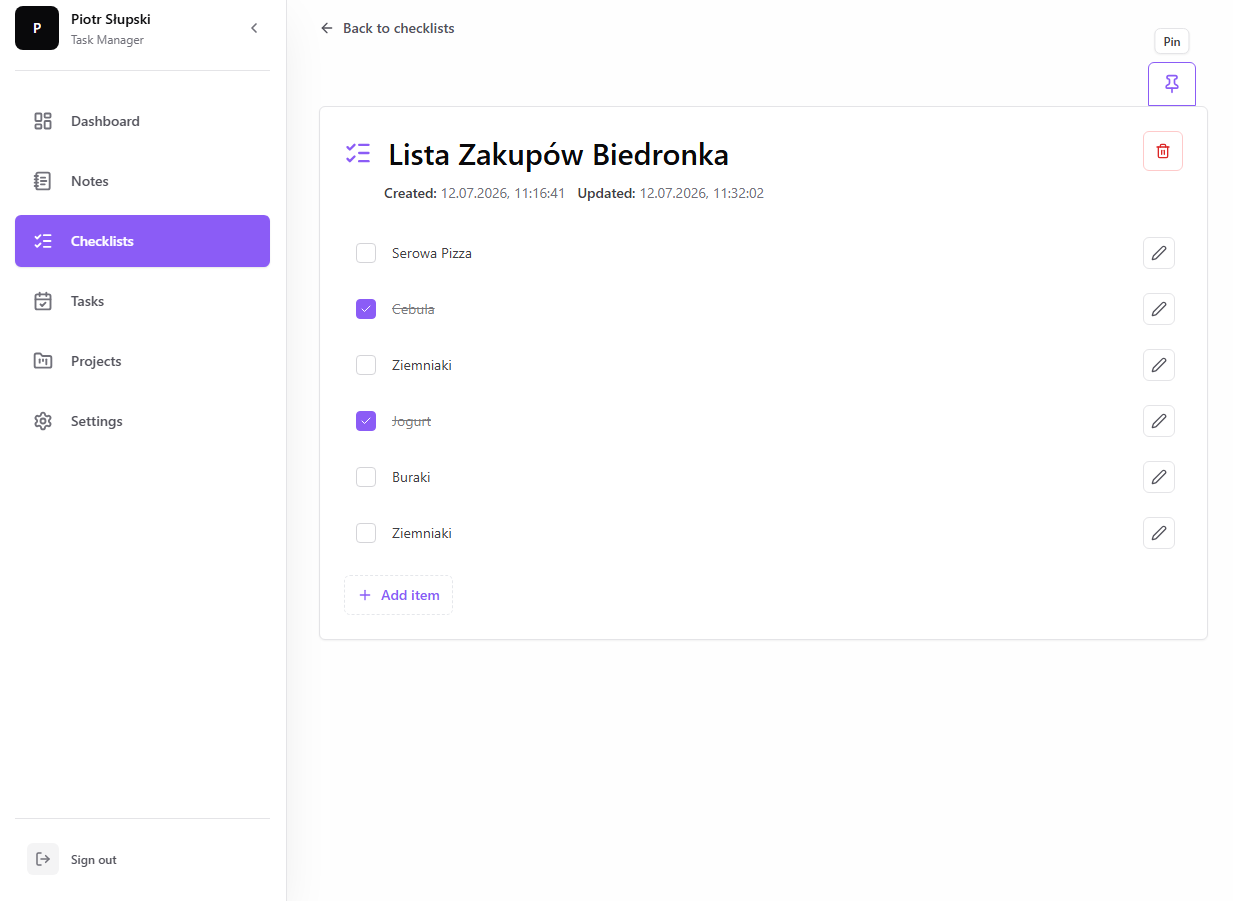
\includegraphics[width=\textwidth,height=0.72\textheight,keepaspectratio]{assets/Scenariusz 1 SS 1.png}
  \caption{Widok, przedstawiający checklistę, z możliwością przypięcia jej do ekranu głównego.}
  \label{fig:scenariusz-1-checklista-przypiecie}
\end{figure}

Na pierwszym z widoków scenariusza pokazano szczegóły checklisty, w których centralnym elementem jest panel z tytułem, datami utworzenia i aktualizacji oraz listą pozycji do odhaczenia. Po prawej stronie umieszczono przyciski akcji, w tym ikonę pinezki służącą do przypięcia checklisty do ekranu głównego. Wykonane elementy checklisty są wyróżnione kolorem oraz przekreśleniem, co pozwala szybko rozpoznać postęp realizacji.

\begin{figure}[H]
  \centering
  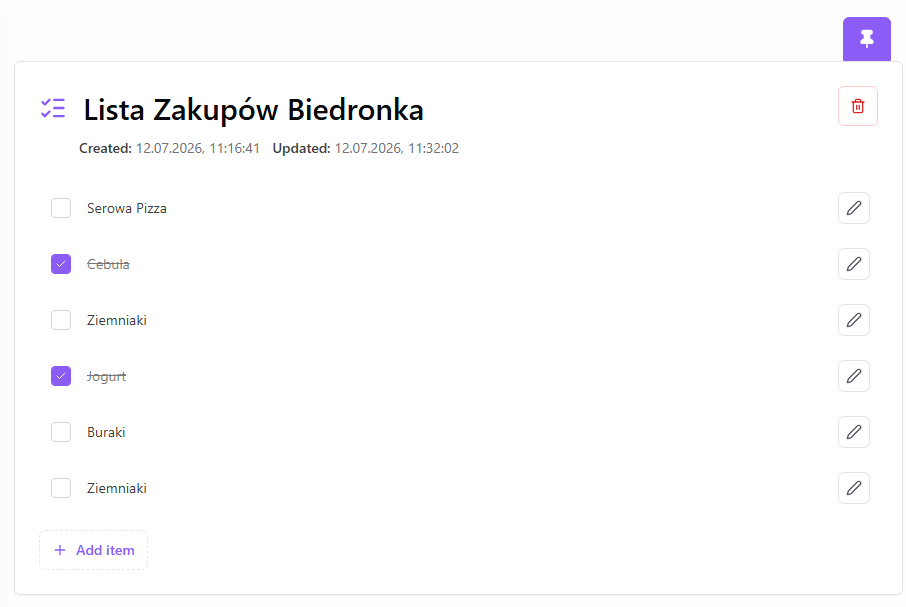
\includegraphics[width=\textwidth,height=0.72\textheight,keepaspectratio]{assets/Scenariusz 1 SS 2.png}
  \caption{Widok przedstawiający zachowanie przycisku ``Przypnij'' po przypięciu checklisty do ekranu głównego.}
  \label{fig:scenariusz-1-przycisk-przypnij}
\end{figure}

Po wykonaniu akcji przypięcia zmienia się wygląd przycisku widocznego przy checkliście. Ikona pinezki zostaje wypełniona kolorem, dzięki czemu interfejs natychmiast informuje, że checklista jest już przypięta. Takie rozwiązanie ogranicza potrzebę dodatkowych komunikatów tekstowych, ponieważ sam stan przycisku staje się informacją zwrotną.

\begin{figure}[H]
  \centering
  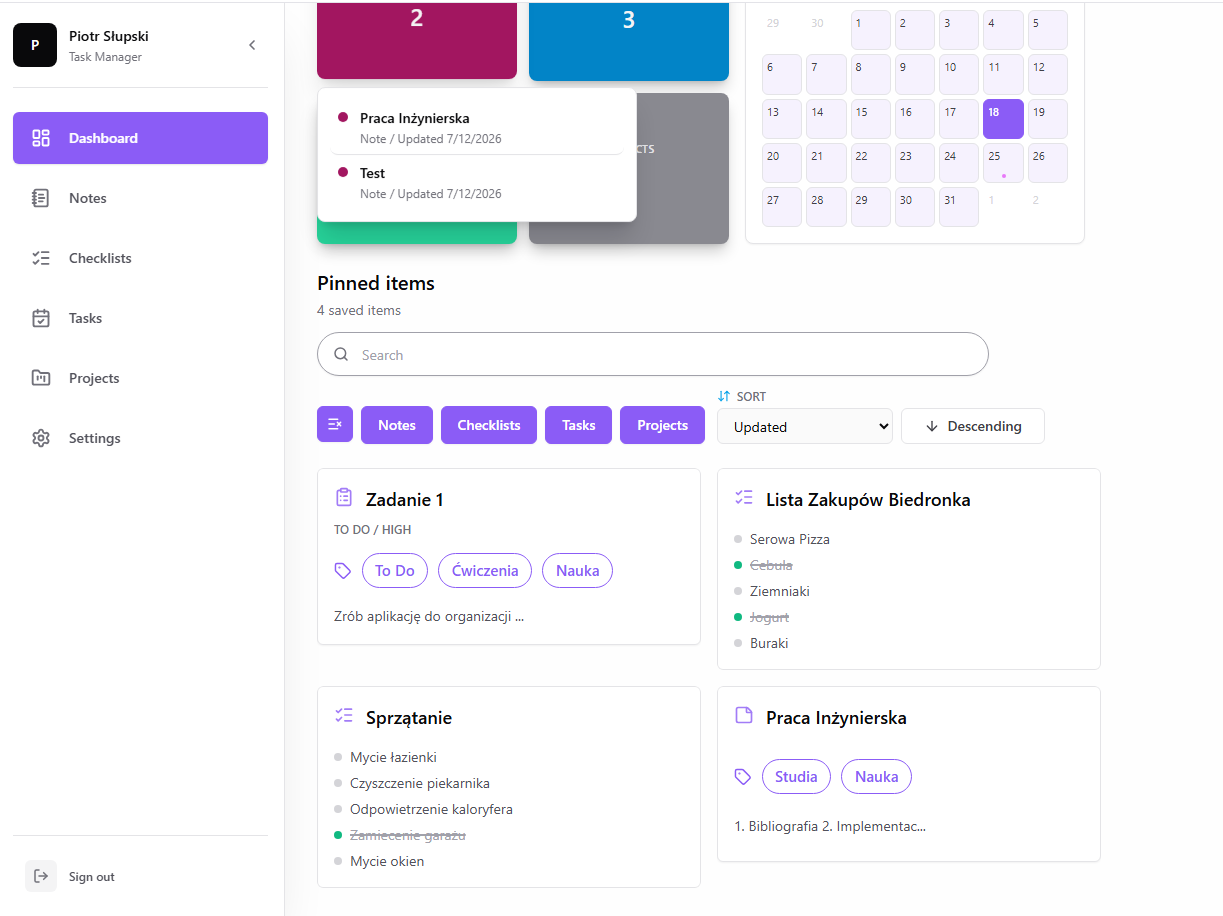
\includegraphics[width=\textwidth,height=0.72\textheight,keepaspectratio]{assets/Scenariusz 1 SS 3.png}
  \caption{Widok przedstawiający elementy przypięte do ekranu głównego.}
  \label{fig:scenariusz-1-przypiete-elementy}
\end{figure}

Sekcja przypiętych elementów na dashboardzie została zorganizowana w formie kart. Elementy przedstawiane są użytkownikowi z ikonami typów, tytułami, tagami oraz skróconym podglądem zawartości. Nad kartami znajduje się menu wyszukiwania, filtrowania i sortowania, dzięki czemu użytkownik może szybko odnaleźć przypięty element bez przechodzenia do osobnych modułów aplikacji.

\begin{figure}[H]
  \centering
  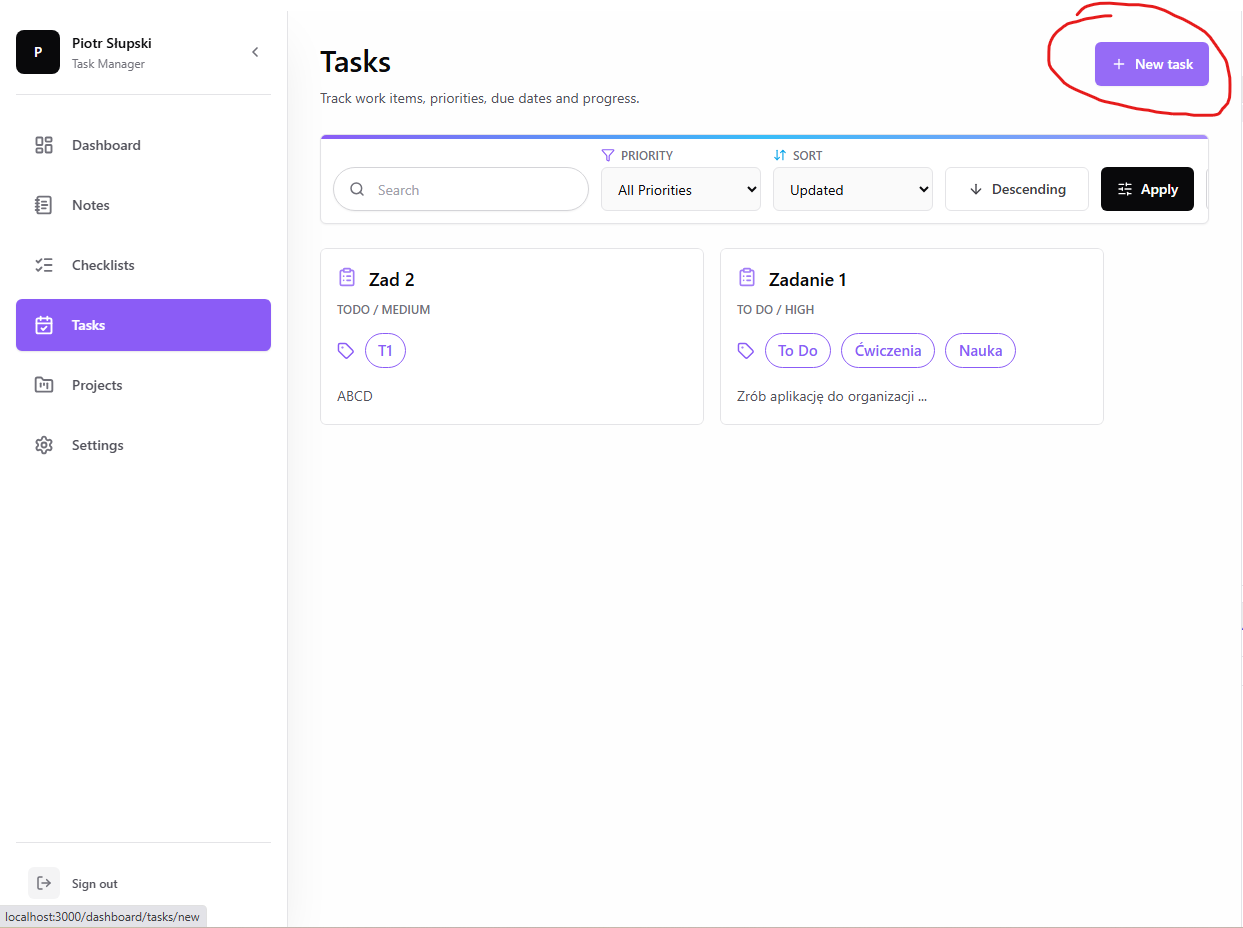
\includegraphics[width=\textwidth,height=0.72\textheight,keepaspectratio]{assets/Scenariusz 2 SS 1.png}
  \caption{Widok, przedstawiający stronę z taskami użytkownika.}
  \label{fig:scenariusz-2-taski}
\end{figure}

Główna strona tasków użytkownika wykorzystuje stały układ z boczną nawigacją i obszarem roboczym. Lewy panel nawigacyjny wskazuje aktywną sekcję aplikacji, a w części roboczej widoczne są nagłówek, opis modułu, pasek filtrowania i sortowania oraz karty tasków. Przycisk utworzenia nowego taska został wyróżniony kolorem akcentu i umieszczony w prawym górnym rogu, co ułatwia rozpoczęcie scenariusza dodawania zadania.

\begin{figure}[H]
  \centering
  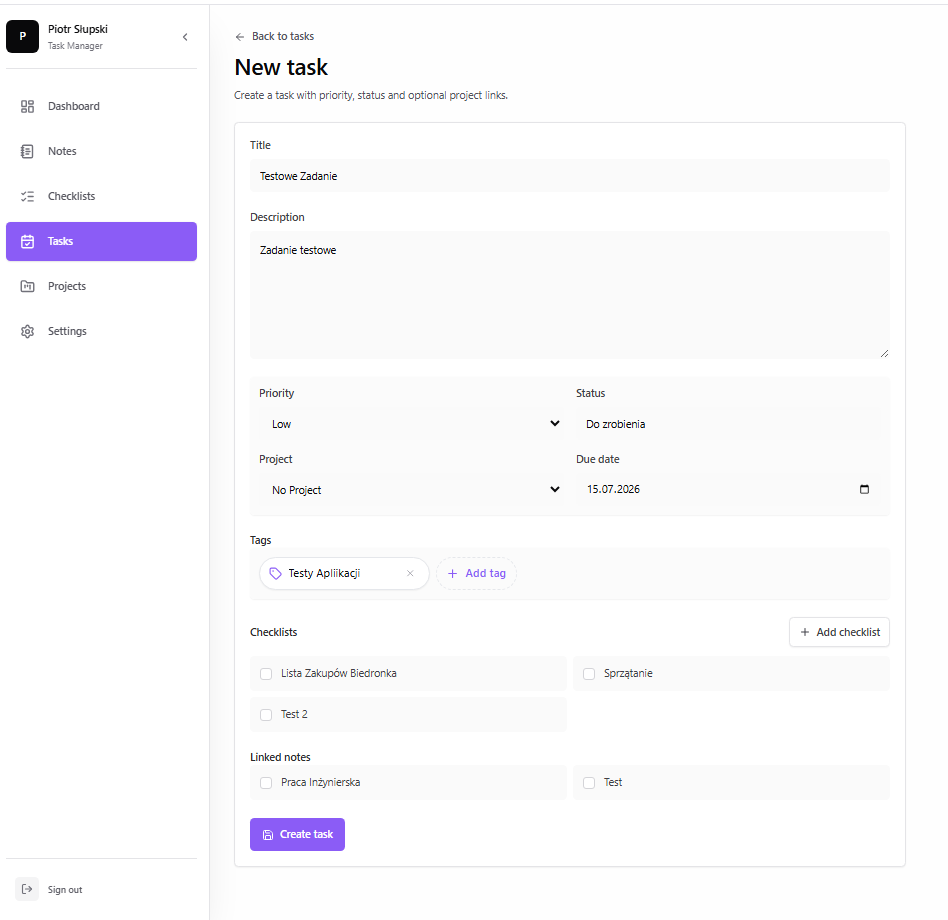
\includegraphics[width=\textwidth,height=0.72\textheight,keepaspectratio]{assets/Scenariusz 2 SS 2.png}
  \caption{Widok, przedstawiający formularz kreacji taska.}
  \label{fig:scenariusz-2-formularz-taska}
\end{figure}

Formularz tworzenia taska uporządkowano według ważności uzupełnianych informacji. Najwyżej umieszczono pola tytułu i opisu, ponieważ są one najważniejsze dla identyfikacji zadania. Niżej znajdują się parametry organizacyjne, takie jak priorytet, status, projekt, termin realizacji, tagi, checklisty oraz powiązane notatki. Formularz zachowuje jednolity układ pól i odstępów, co zwiększa czytelność nawet przy większej liczbie ustawień.

\begin{figure}[H]
  \centering
  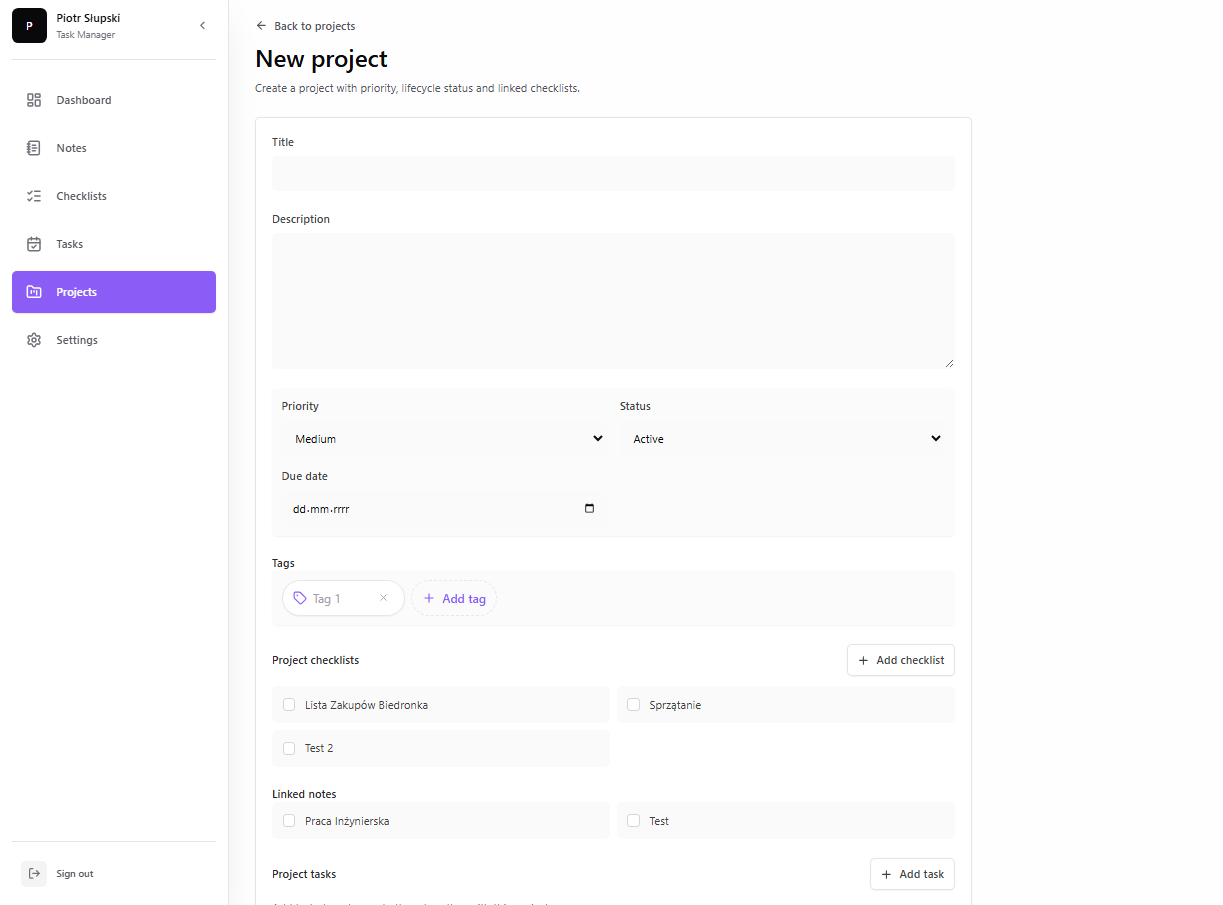
\includegraphics[width=\textwidth,height=0.72\textheight,keepaspectratio]{assets/Scenariusz 5 SS 1.png}
  \caption{Widok przedstawiający pierwszą część formularza kreacji projektu.}
  \label{fig:scenariusz-5-formularz-projektu-pierwsza-czesc}
\end{figure}

Pierwsza część formularza projektu skupia się na podstawowych danych opisowych. Widoczne są pola takie jak tytuł, opis, priorytet, status, termin realizacji oraz tagi. W dalszej części ekranu znajdują się również powiązania z checklistami i notatkami, co pokazuje, że projekt może grupować różne typy informacji potrzebnych do organizacji pracy.

\begin{figure}[H]
  \centering
  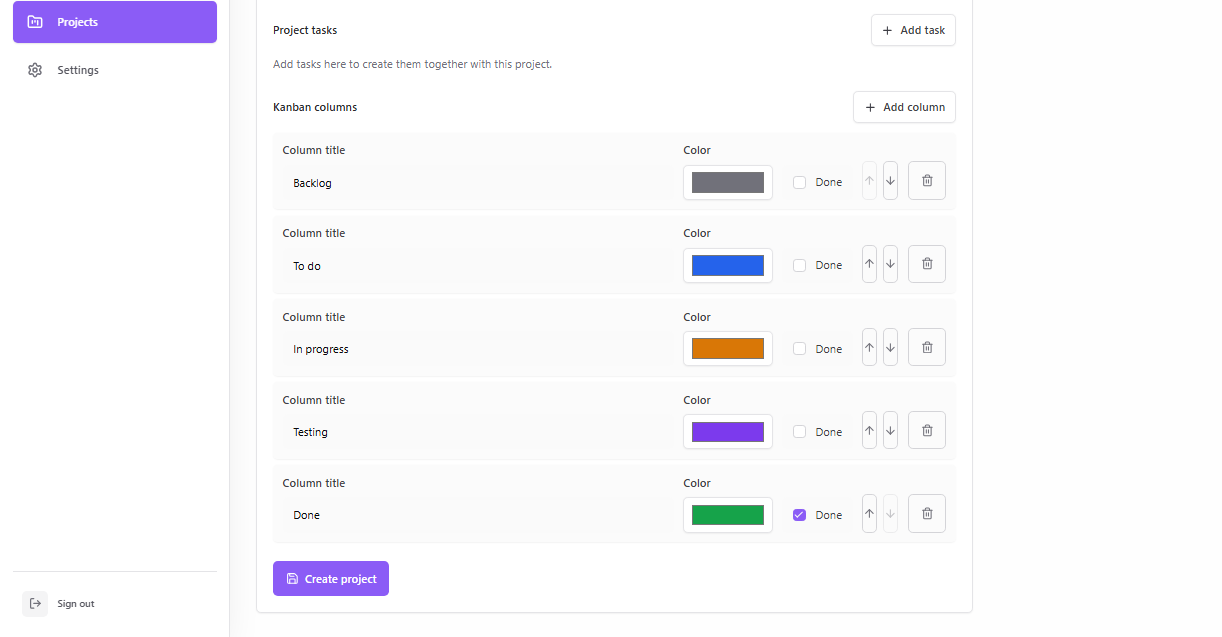
\includegraphics[width=\textwidth,height=0.72\textheight,keepaspectratio]{assets/Scenariusz 5 SS 2.png}
  \caption{Widok przedstawiający drugą część formularza kreacji projektu.}
  \label{fig:scenariusz-5-formularz-projektu-druga-czesc}
\end{figure}

W drugiej części formularza użytkownik może skonfigurować kolumny tablicy kanban. Każda kolumna jest przedstawiona jako osobny wiersz z nazwą, kolorem, oznaczeniem stanu zakończonego oraz przyciskami zmiany kolejności i usunięcia. Dzięki temu struktura przyszłej tablicy projektu jest widoczna jeszcze przed zapisaniem projektu.

\begin{figure}[H]
  \centering
  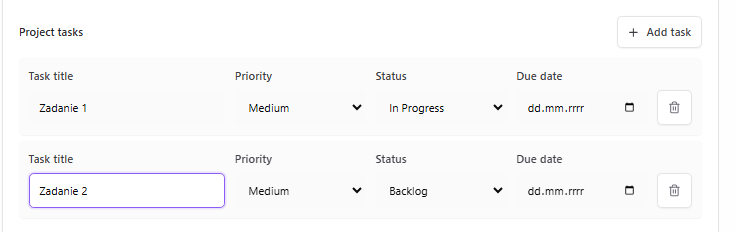
\includegraphics[width=\textwidth,height=0.72\textheight,keepaspectratio]{assets/Scenariusz 5 SS 3 .png}
  \caption{Widok, przedstawiający opcję dodawania tasków do projektu.}
  \label{fig:scenariusz-5-dodawanie-taskow}
\end{figure}

Sekcja dodawania tasków pozwala uzupełnić podzadania bezpośrednio podczas tworzenia projektu. Poszczególne taski zostały ułożone w wierszach, a każdy z nich posiada pola tytułu, priorytetu, statusu i terminu realizacji. Taki układ pozwala użytkownikowi szybko porównać kilka podzadań i przypisać im początkowe statusy jeszcze przed utworzeniem projektu.

\begin{figure}[H]
  \centering
  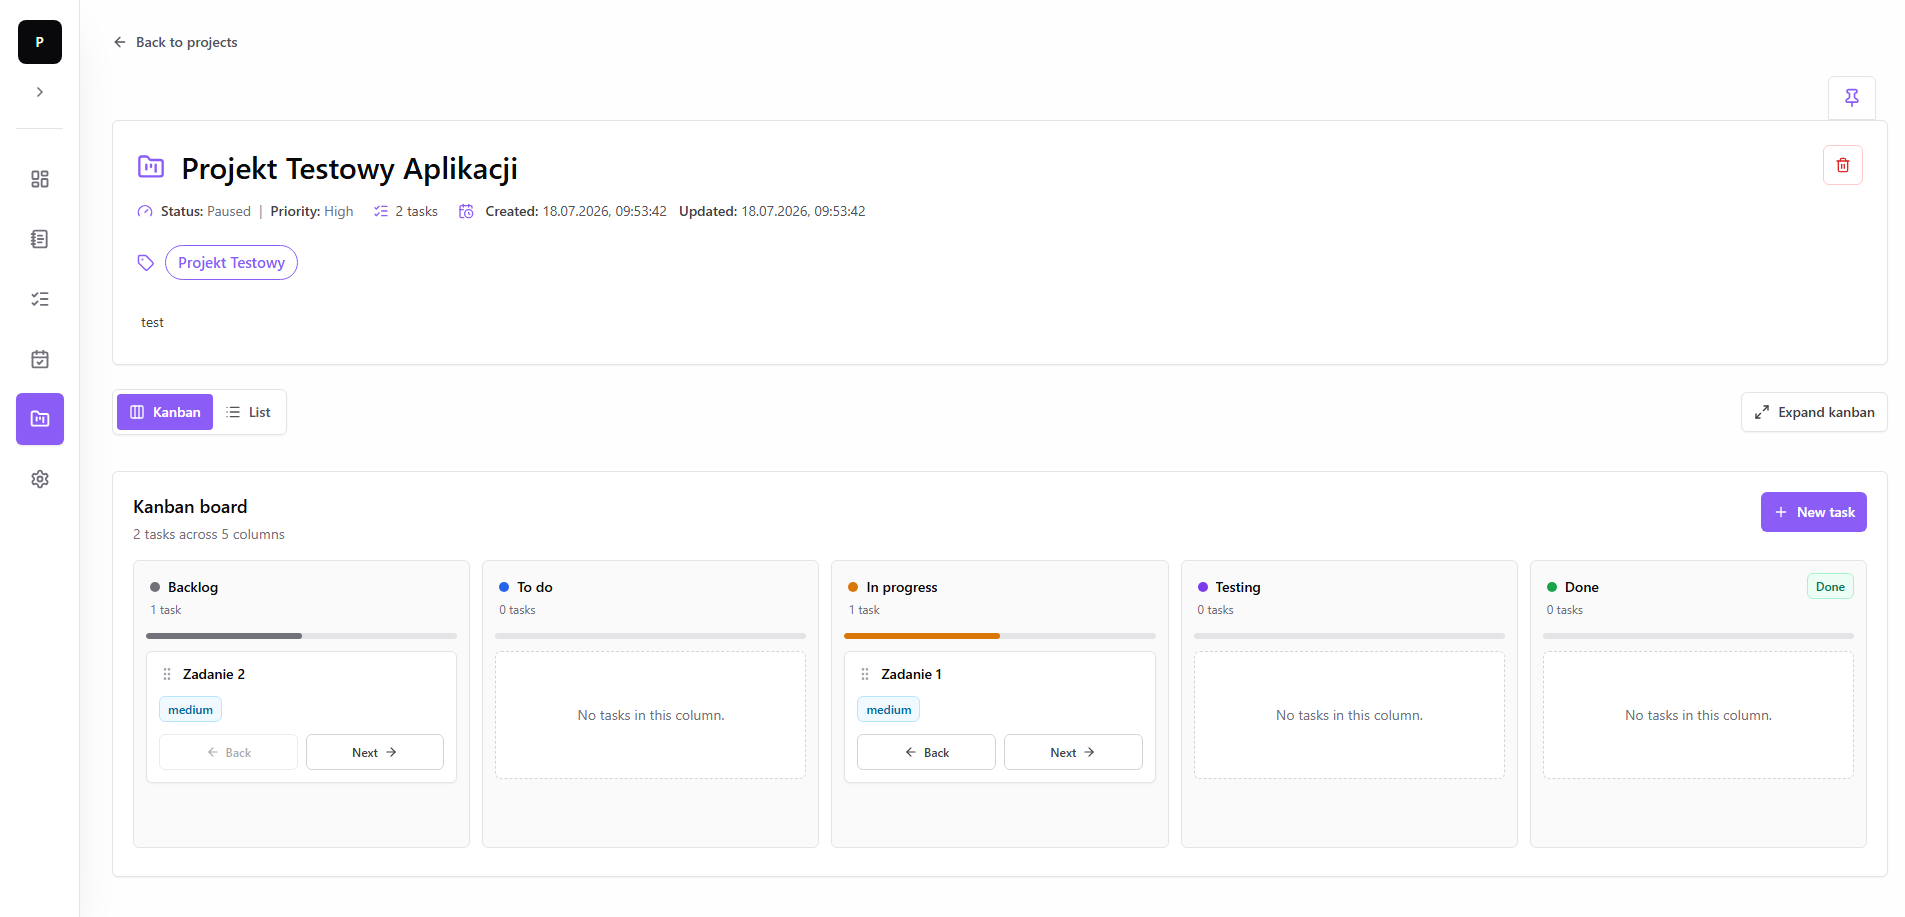
\includegraphics[width=\textwidth,height=0.72\textheight,keepaspectratio]{assets/Scenariusz 5 SS 4.png}
  \caption{Widok, przedstawiający tablicę kanban projektu.}
  \label{fig:scenariusz-5-tablica-kanban}
\end{figure}

Widok tablicy kanban prezentuje projekt jako zestaw kolumn odpowiadających statusom zadań. Zadania są rozmieszczone w kolumnach, a kolorowe oznaczenia nagłówków pomagają odróżnić poszczególne etapy pracy. Karty tasków zawierają najważniejsze informacje, takie jak tytuł i priorytet, a przyciski przejścia do poprzedniej lub następnej kolumny wspierają zmianę statusu zadania.

\begin{figure}[H]
  \centering
  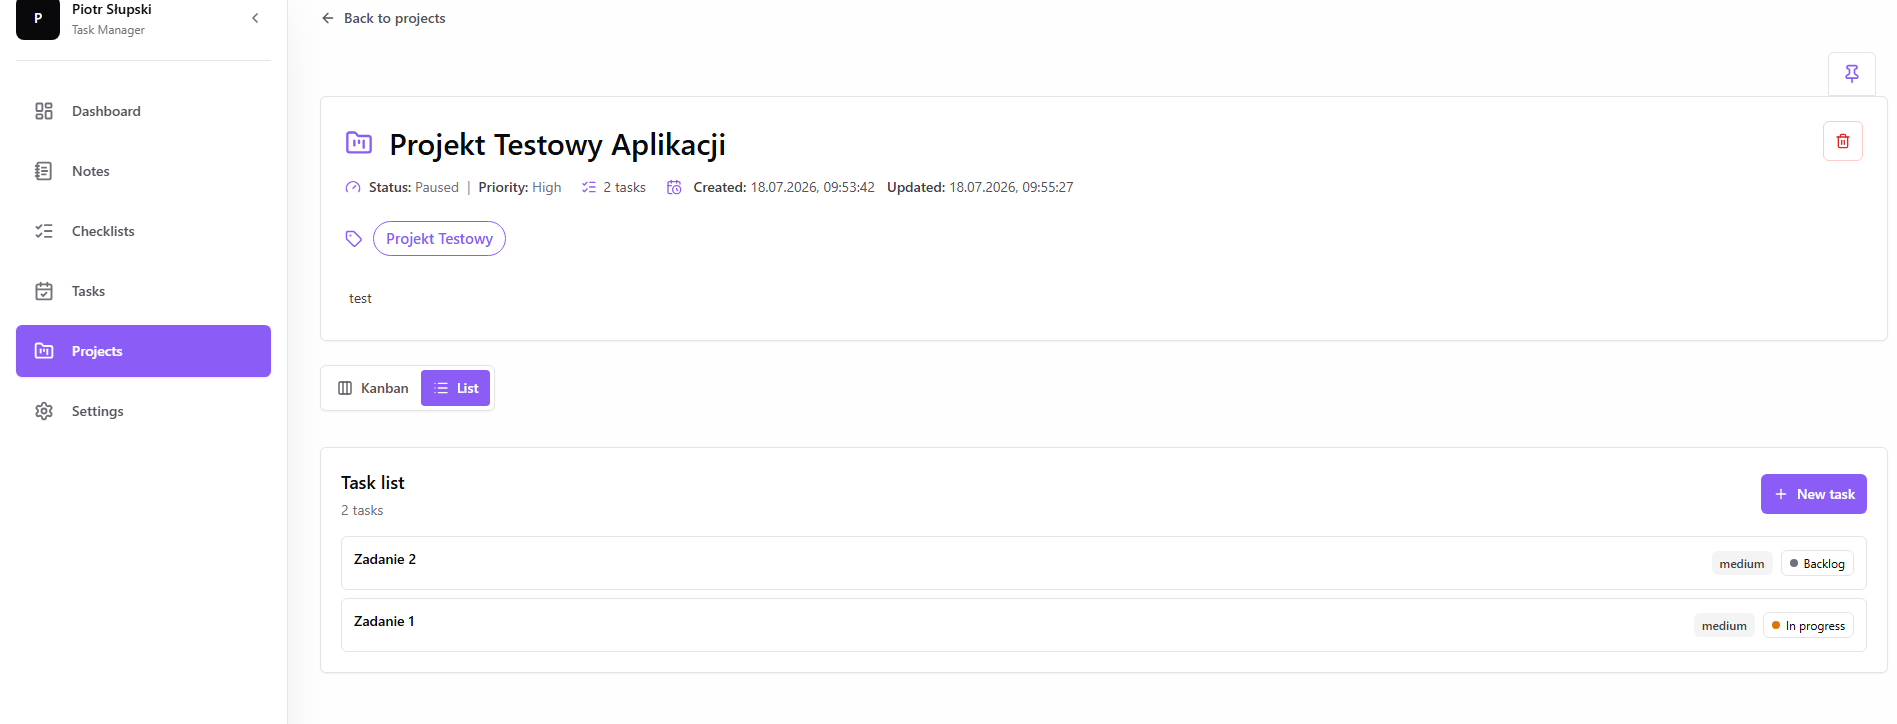
\includegraphics[width=\textwidth,height=0.72\textheight,keepaspectratio]{assets/Scenariusz 5 SS 5.png}
  \caption{Widok, przedstawiający taski projektów w formie listy.}
  \label{fig:scenariusz-5-lista-taskow-projektu}
\end{figure}

Alternatywny widok tasków projektu przyjmuje formę listy. W tym układzie zadania są pokazane jako poziome wiersze, dzięki czemu użytkownik może szybko przejrzeć ich nazwy, priorytety oraz aktualne statusy. Przełącznik pomiędzy widokiem kanban i listą znajduje się nad obszarem tasków, co pozwala dobrać sposób prezentacji danych do aktualnego trybu pracy.

\chapter{Implementacja kodu po stronie frontendu}

\FirstParagraph W niniejszym rozdziale opisano wybrane elementy implementacji warstwy frontendowej aplikacji. Skupiono się na dwóch częściach systemu, które mają szczególne znaczenie dla ergonomii pracy użytkownika: widoku kanban w projekcie oraz sekcji przypiętych elementów na dashboardzie. Oba fragmenty zostały zaimplementowane jako komponenty React działające w środowisku Next.js i komunikujące się z backendem za pomocą endpointów API.

\section{Implementacja widoku kanban}

\FirstParagraph Widok kanban został zaimplementowany głównie w komponencie \texttt{ProjectKanbanBoard}, znajdującym się w pliku \texttt{project-kanban-board.tsx}. Komponent ten odpowiada za wyświetlanie tablicy projektu, kolumn statusów oraz kart zadań. Dane wejściowe przekazywane do komponentu obejmują identyfikator projektu, listę kolumn oraz listę zadań. Dzięki temu komponent nie pobiera danych samodzielnie, lecz otrzymuje je z warstwy strony projektu, co upraszcza jego odpowiedzialność i pozwala wykorzystać renderowanie po stronie serwera dla początkowego stanu widoku.

Każda kolumna kanban jest reprezentowana przez obiekt zawierający identyfikator, nazwę, kolor oraz informację, czy dana kolumna oznacza zadanie zakończone. Zadanie zawiera między innymi identyfikator, tytuł, opis, priorytet, aktualny status, pozycję, termin oraz tagi. Relacja pomiędzy zadaniem i kolumną jest realizowana przez pole \texttt{statusId}. Jeżeli \texttt{statusId} zadania jest równe identyfikatorowi kolumny, karta zadania zostaje wyrenderowana właśnie w tej kolumnie.

Komponent utrzymuje lokalny stan tablicy za pomocą hooków \texttt{useState}. W stanie przechowywane są między innymi aktualne zadania, kolumny, identyfikator przenoszonego zadania, informacja o aktywnej kolumnie upuszczania oraz dane edytowanej kolumny. Dodatkowo zastosowano \texttt{useEffect}, aby synchronizować lokalny stan komponentu z danymi przekazanymi przez stronę projektu. Dzięki temu po odświeżeniu danych przez router widok zostaje zaktualizowany zgodnie ze stanem zapisanym w bazie.

Lista kolumn jest wyliczana w \texttt{useMemo}. Jeżeli projekt nie posiada zdefiniowanych kolumn, komponent tworzy kolumnę domyślną \texttt{todo}. Dodatkowo sprawdzane są statusy istniejących zadań. Jeżeli zadanie posiada status, którego nie ma w konfiguracji projektu, tworzona jest dodatkowa kolumna techniczna. Takie rozwiązanie zabezpiecza interfejs przed sytuacją, w której zadanie miałoby zniknąć z tablicy tylko dlatego, że jego status nie występuje już w konfiguracji kolumn.

Przenoszenie zadania między kolumnami zostało zaimplementowane na dwa sposoby. Pierwszym jest mechanizm \texttt{drag and drop}, w którym funkcje \texttt{handleDragStart}, \texttt{handleDragOver} i \texttt{handleDrop} obsługują przeciąganie karty oraz upuszczanie jej w wybranej kolumnie. Drugim sposobem są przyciski \texttt{Back} i \texttt{Next}, które przenoszą zadanie do poprzedniej lub następnej kolumny. Dzięki temu widok pozostaje użyteczny również wtedy, gdy użytkownik nie chce korzystać z przeciągania.

Za właściwą zmianę statusu odpowiada funkcja \texttt{moveTask}. Po wybraniu nowej kolumny funkcja oblicza następną pozycję zadania w tej kolumnie, aktualizuje lokalny stan tablicy i wysyła żądanie \texttt{PATCH} do endpointu \texttt{/api/tasks/\{taskId\}}. W treści żądania przekazywane są \texttt{statusId}, \texttt{projectId} oraz \texttt{position}. Aktualizacja lokalnego stanu wykonywana jest przed odpowiedzią serwera, co daje użytkownikowi wrażenie natychmiastowej reakcji interfejsu. Jeżeli backend zwróci błąd, komponent przywraca poprzedni stan zadań i wyświetla komunikat o niepowodzeniu operacji.

Istotnym elementem implementacji jest również edycja kolumn. Użytkownik może kliknąć nagłówek kolumny, zmienić jej nazwę, kolor oraz oznaczyć ją jako kolumnę końcową. Po zapisaniu zmian komponent wysyła żądanie \texttt{PATCH} do endpointu \texttt{/api/projects/\{projectId\}}, przekazując zaktualizowaną tablicę \texttt{kanbanColumns}. Każda kolumna otrzymuje także pozycję wynikającą z kolejności w tablicy. Po poprawnym zapisie wykonywane jest \texttt{router.refresh()}, co odświeża dane projektu.

Widok kanban jest osadzony w komponencie \texttt{ProjectTaskView}. Ten komponent pozwala przełączać sposób prezentacji zadań między widokiem \texttt{kanban} i widokiem \texttt{list}. Wybrany tryb jest zapisywany w projekcie przez żądanie \texttt{PATCH} do endpointu projektu, w polu \texttt{taskView}. Dzięki temu wybór użytkownika nie jest wyłącznie stanem tymczasowym w przeglądarce, ale częścią konfiguracji projektu przechowywaną w bazie danych. Dodatkowo dla tablicy kanban dostępny jest tryb rozszerzony, który wyświetla tablicę na całym ekranie i ułatwia pracę z większą liczbą zadań.

Karty zadań w widoku kanban zawierają najważniejsze informacje potrzebne do szybkiej oceny pracy: tytuł, skrócony opis, priorytet, termin oraz tagi. Priorytety są wyróżnione kolorami, a termin jest prezentowany razem z ikoną kalendarza. Każda karta jest linkiem do szczegółów zadania, dzięki czemu użytkownik może szybko przejść z ogólnego widoku projektu do edycji konkretnego elementu.

\section{Implementacja sekcji przypiętych elementów dashboardu}

\FirstParagraph Sekcja przypiętych elementów dashboardu została oparta na kolekcji \texttt{pins}, która przechowuje identyfikator użytkownika, typ przypiętego elementu, identyfikator celu oraz pozycję. Frontend nie przechowuje osobnych list przypiętych notatek, zadań, checklist i projektów. Zamiast tego każdy pin zawiera parę \texttt{targetType} oraz \texttt{targetId}, która pozwala wskazać dowolny obsługiwany typ elementu.

Pobieranie danych do dashboardu odbywa się w pliku \texttt{dashboard/page.tsx}. Strona najpierw sprawdza sesję użytkownika, a następnie łączy się z bazą danych. Za pomocą \texttt{Promise.all} równolegle pobierane są przypięcia, liczniki głównych typów danych, ostatnio aktualizowane notatki, checklisty, zadania i projekty oraz wydarzenia kalendarza wynikające z terminów zadań i projektów. Takie podejście ogranicza czas oczekiwania na dane, ponieważ niezależne zapytania są wykonywane równocześnie.

Dla każdego dokumentu \texttt{Pin} wykonywana jest funkcja \texttt{findPinnedTarget}. Funkcja ta sprawdza typ przypięcia i na tej podstawie pobiera właściwy dokument z kolekcji \texttt{notes}, \texttt{checklists}, \texttt{tasks} albo \texttt{projects}. Każde zapytanie zawiera warunek \texttt{ownerId} oraz \texttt{archivedAt: null}, dlatego dashboard pokazuje tylko aktywne elementy należące do zalogowanego użytkownika. Jeżeli przypięty dokument nie istnieje lub został zarchiwizowany, nie jest przekazywany do interfejsu.

Po pobraniu celu przypięcia dane są mapowane do wspólnego formatu \texttt{PinnedItem}. Obiekt ten zawiera tytuł, opis, typ, status, priorytet, tagi, daty utworzenia i aktualizacji oraz link prowadzący do szczegółów elementu. Dzięki ujednoliceniu danych komponenty frontendowe mogą renderować przypięte notatki, checklisty, zadania i projekty w jednej sekcji, bez konieczności tworzenia czterech osobnych widoków.

Głównym komponentem dashboardu jest \texttt{PinnedBoard}. Renderuje on kafelki metryk, mały kalendarz oraz komponent \texttt{PinnedItemsSearch}. Kafelki metryk pokazują liczbę notatek, checklist, zadań i projektów. Po najechaniu na kafelek wyświetlana jest lista ostatnio aktualizowanych elementów danego typu. Kalendarz jest budowany lokalnie na podstawie zadań i projektów mających termin w bieżącym miesiącu. Funkcja \texttt{buildCalendarDays} tworzy siatkę dni, oznacza aktualny dzień oraz przypisuje wydarzenia do odpowiednich dat.

Za właściwą listę przypiętych elementów odpowiada komponent \texttt{PinnedItemsSearch}. Komponent ten działa po stronie klienta, ponieważ obsługuje stan wyszukiwarki, filtrów oraz sortowania. Użytkownik może wyszukiwać przypięte elementy po tytule, opisie, typie, statusie i metadanych. Może także filtrować wyniki według typu elementu: notatek, checklist, zadań lub projektów. Lista typów jest przechowywana w stanie \texttt{selectedTypes}, a filtrowanie wykonywane jest w \texttt{useMemo}, aby nie przeliczać wyników bez potrzeby przy każdym renderowaniu.

Sortowanie przypiętych elementów obsługuje stan \texttt{sortField} oraz \texttt{sortDirection}. Użytkownik może sortować elementy po dacie aktualizacji, dacie utworzenia, tytule lub opisie. Dla pól tekstowych domyślnym kierunkiem jest sortowanie rosnące, natomiast dla dat domyślnie pokazywane są najnowsze elementy. Wyniki po filtrowaniu są kopiowane do nowej tablicy i sortowane bez modyfikowania danych wejściowych przekazanych do komponentu.

Każdy przypięty element jest renderowany jako karta \texttt{ObjectCard}. Ikona karty zależy od typu elementu: notatka, checklista, zadanie lub projekt. Dla zadań i projektów przekazywany jest status oraz priorytet, natomiast dla checklist możliwe jest pokazanie podglądu elementów checklisty. Link karty prowadzi bezpośrednio do szczegółowego widoku danego elementu.

Za przypinanie i odpinanie odpowiada komponent przycisku pinezki, wydzielony w kodzie jako \texttt{PinEntityButton}. Komponent otrzymuje typ i identyfikator elementu oraz opcjonalny identyfikator istniejącego przypięcia. Jeżeli element nie jest przypięty, kliknięcie wysyła żądanie \texttt{POST} do endpointu \texttt{/api/pins}. Jeżeli element jest już przypięty, kliknięcie wysyła żądanie \texttt{DELETE} do endpointu \texttt{/api/pins/\{pinId\}}. Po poprawnym zakończeniu operacji komponent aktualizuje lokalny stan, zmienia wygląd ikony pinezki oraz wykonuje \texttt{router.refresh()}, aby odświeżyć dashboard i pozostałe widoki.

W efekcie sekcja przypiętych elementów pełni rolę spersonalizowanego skrótu do najważniejszych danych użytkownika. Implementacja została oparta na jednym wspólnym modelu przypięcia oraz na uniwersalnym komponencie listującym, dzięki czemu dodanie obsługi kolejnego typu elementu wymagałoby głównie rozszerzenia mapowania typów i sposobu pobierania celu przypięcia.

\chapter{Implementacja kodu po stronie backendu}

\FirstParagraph W niniejszym rozdziale opisano wybrane elementy implementacji backendu aplikacji. Skupiono się na dwóch obszarach istotnych dla działania systemu: obsłudze checklist przez API oraz mechanizmie autoryzacji użytkownika. Oba fragmenty są wykonywane po stronie serwera, dlatego odpowiadają za sprawdzanie dostępu do danych, walidację żądań oraz komunikację z bazą danych.

\section{Implementacja handlera API checklist}

\FirstParagraph Obsługa checklist została zaimplementowana w dwóch routach API: listowym oraz dynamicznym dla pojedynczej checklisty. Pierwszy route odpowiada za operacje wykonywane na całej kolekcji checklist, natomiast drugi za operacje dotyczące pojedynczej checklisty wskazanej przez identyfikator w adresie żądania. Takie rozdzielenie wynika ze sposobu działania mechanizmu routingu w Next.js, w którym struktura katalogów określa ścieżki dostępne w API.

W pliku \texttt{route.ts} zdefiniowano metody \texttt{GET} oraz \texttt{POST}. Metoda \texttt{GET} pobiera listę aktywnych checklist należących do aktualnie zalogowanego użytkownika. Przed wykonaniem zapytania do bazy wywoływana jest funkcja \texttt{getCurrentUserId}, która zwraca identyfikator użytkownika zapisany w sesji. Jeżeli identyfikator nie jest dostępny, handler\footnote{Handler - funkcja obsługująca określony typ żądania przychodzącego do aplikacji, np. pobranie, utworzenie lub aktualizację danych.} kończy działanie odpowiedzią \texttt{401 Unauthorized}.

Po pozytywnej weryfikacji użytkownika wykonywane jest połączenie z bazą danych przez funkcję \texttt{connectDatabase}. Następnie model \texttt{Checklist} wyszukuje dokumenty spełniające warunki \texttt{ownerId} oraz \texttt{archivedAt: null}. Oznacza to, że użytkownik otrzymuje tylko własne checklisty, które nie zostały wcześniej zarchiwizowane. Wyniki są sortowane według pola \texttt{position}, a następnie według daty aktualizacji, dzięki czemu interfejs może prezentować elementy w ustalonej kolejności.

Metoda \texttt{POST} odpowiada za utworzenie nowej checklisty. Treść żądania jest odczytywana za pomocą funkcji \texttt{parseJsonBody}, która jednocześnie korzysta ze schematu \texttt{checklistCreateSchema}. Schemat waliduje tytuł checklisty, elementy checklisty, typ i identyfikator elementu nadrzędnego oraz pozycję. W przypadku niepoprawnych danych handler zwraca odpowiedź błędu i nie wykonuje zapisu w bazie danych.

Przed utworzeniem dokumentu dane są przekazywane do funkcji \texttt{sanitizeMutation}. Jej zadaniem jest ograniczenie zapisywanych wartości do pól dopuszczonych przez logikę aplikacji. Następnie model \texttt{Checklist} tworzy dokument z danymi użytkownika oraz identyfikatorem właściciela. Po poprawnym zapisie wywoływana jest funkcja \texttt{recordActivityEvent}, która rejestruje zdarzenie utworzenia checklisty w historii aktywności.

Operacje na pojedynczej checkliście znajdują się w dynamicznej ścieżce API, w której identyfikator checklisty jest częścią adresu żądania. W metodach \texttt{GET}, \texttt{PATCH} i \texttt{DELETE} najpierw sprawdzana jest sesja użytkownika, a następnie poprawność identyfikatora checklisty za pomocą funkcji \texttt{isValidObjectId}. Dzięki temu aplikacja nie wykonuje zapytań do bazy dla niepoprawnie zbudowanych identyfikatorów.

Metoda \texttt{PATCH} aktualizuje checklistę przy użyciu schematu \texttt{checklistUpdateSchema}. Schemat ten dopuszcza częściową aktualizację, ale wymaga przekazania przynajmniej jednego pola. Aktualizacja wykonywana jest przez \texttt{findOneAndUpdate} z warunkami \texttt{\_id}, \texttt{ownerId} oraz \texttt{archivedAt: null}. Taki zapis zabezpiecza przed zmianą checklist należących do innych użytkowników oraz przed modyfikacją elementów zarchiwizowanych.

Usunięcie checklisty zostało zrealizowane jako archiwizacja. Metoda \texttt{DELETE} nie usuwa dokumentu fizycznie z bazy, lecz zapisuje w polu \texttt{archivedAt} aktualną datę. Dzięki temu dane nie są widoczne w standardowych zapytaniach, ale w razie potrzeby możliwe byłoby zachowanie historii działania systemu. Po aktualizacji dokumentu rejestrowane jest zdarzenie usunięcia checklisty.

\section{Implementacja API odpowiedzialnego za autoryzację}

\FirstParagraph Mechanizm autoryzacji został oparty na bibliotece Auth.js, używanej w projekcie przez pakiet NextAuth. Główny handler autoryzacji znajduje się w dynamicznej ścieżce API przeznaczonej dla NextAuth. Plik ten tworzy handler NextAuth na podstawie konfiguracji \texttt{authOptions}, a następnie udostępnia go dla metod \texttt{GET} i \texttt{POST}. Dzięki temu biblioteka może obsługiwać zarówno rozpoczęcie logowania, jak i odpowiedzi zwrotne od dostawców OAuth.

Konfiguracja autoryzacji została umieszczona w pliku \texttt{src/lib/auth.ts}. Zdefiniowano w nim listę dostawców logowania OAuth, obejmującą Google oraz GitHub. Każdy dostawca posiada identyfikator, nazwę, dane klienta pobierane ze zmiennych środowiskowych oraz funkcję tworzącą konfigurację providera. Aplikacja uruchamia tylko tych dostawców, dla których dostępne są wymagane dane \texttt{clientId} i \texttt{clientSecret}.

W przypadku logowania z użyciem zewnętrznych dostawców ważne jest nie tylko samo przekazanie użytkownika do usługi logowania, ale również poprawne obsłużenie odpowiedzi zwrotnej, tokenów oraz powiązania konta z lokalnym użytkownikiem aplikacji. Sun i Beznosov, analizując systemy jednokrotnego logowania oparte na OAuth, zwracają uwagę, że wiele problemów bezpieczeństwa wynika nie z idei protokołu, lecz z decyzji implementacyjnych podejmowanych przez twórców aplikacji\footnote{Sun S.-T., Beznosov K., \emph{The Devil is in the (Implementation) Details: An Empirical Analysis of OAuth SSO Systems}, w: \emph{Proceedings of the 2012 ACM Conference on Computer and Communications Security}, 2012, s. 378--390, DOI: 10.1145/2382196.2382238, \url{https://doi.org/10.1145/2382196.2382238} (dostęp: 31.07.2026).}. Z tego względu w projekcie autoryzacja została skupiona w jednym module konfiguracyjnym, a pozostałe handler API korzystają z jednolitej funkcji zwracającej identyfikator aktualnego użytkownika.

Do przechowywania danych autoryzacyjnych wykorzystano adapter MongoDB. Adapter zapisuje w bazie informacje o użytkownikach i powiązanych kontach zewnętrznych, dzięki czemu aplikacja może rozpoznawać tę samą osobę po kolejnych logowaniach. Dane te są przechowywane w kolekcjach technicznych tworzonych przez mechanizm NextAuth, niezależnie od domenowych kolekcji aplikacji, takich jak taski, checklisty czy projekty.

Sesja użytkownika działa w strategii \texttt{jwt}. JWT\footnote{JWT - skrót od JSON Web Token; jest to format tokenu używany do przenoszenia informacji o użytkowniku lub uprawnieniach między stronami komunikacji.} pozwala przechowywać podstawowe informacje o zalogowanym użytkowniku w tokenie sesyjnym. W konfiguracji zastosowano callback \texttt{session}, który przenosi identyfikator użytkownika z tokenu do obiektu \texttt{session.user.id}. Dzięki temu pozostałe części backendu mogą korzystać z jednolitego sposobu identyfikacji właściciela danych.

W praktyce autoryzacja jest używana w handlerach API przez funkcję pobierającą identyfikator aktualnego użytkownika. Każda operacja na danych użytkownika rozpoczyna się od pobrania identyfikatora sesji. Następnie identyfikator ten trafia do warunków zapytań jako \texttt{ownerId}. Takie rozwiązanie sprawia, że nawet poprawnie zbudowane żądanie nie pozwala odczytać ani zmienić danych należących do innej osoby.

\chapter{Testy jednostkowe}

\FirstParagraph Test jednostkowy sprawdza niewielki, wydzielony fragment programu, np. funkcję lub schemat walidacji, bez uruchamiania całego systemu. Testy jednostkowe służą więc do weryfikowania małych części aplikacji w kontrolowanych warunkach. Ich zadaniem jest szybkie wykrywanie błędów w logice programu oraz zabezpieczenie już działających funkcji przed przypadkowymi regresjami podczas dalszego rozwoju projektu.

W aplikacji testy zostały uruchamiane za pomocą narzędzia Vitest, które jest dostosowane do testowania kodu JavaScript i TypeScript. Dokumentacja Vitest wskazuje, że test opisuje oczekiwane zachowanie wybranego fragmentu kodu, a funkcje \texttt{test} oraz \texttt{expect} pozwalają definiować sprawdzane przypadki i porównywać wynik działania programu z oczekiwanym rezultatem\footnote{Vitest, \emph{Writing Tests}, dostęp: \url{https://vitest.dev/guide/learn/writing-tests.html} (03.08.2026).}. W kontekście aplikacji React podobną rolę pełnią narzędzia pozwalające renderować komponenty w środowisku testowym i sprawdzać widoczne dla użytkownika elementy interfejsu; dokumentacja React Testing Library opisuje m.in. funkcję \texttt{render}, służącą do osadzania komponentu w kontenerze testowym\footnote{Testing Library, \emph{React Testing Library API}, dostęp: \url{https://testing-library.com/docs/react-testing-library/api/} (03.08.2026).}.

\section{Testy funkcjonalności tasków}

\FirstParagraph Dla funkcjonalności tasków dodano testy jednostkowe w pliku \texttt{task-validation.test.ts}. Testy koncentrują się na schematach \texttt{taskCreateSchema} oraz \texttt{taskUpdateSchema}, ponieważ to one decydują, jakie dane mogą zostać przyjęte przez API odpowiedzialne za tworzenie i aktualizowanie tasków.

Pierwszy test sprawdza poprawny, pełny zestaw danych taska. Weryfikowane są między innymi tytuł, opis, priorytet, status, identyfikator projektu, termin, tagi, powiązane checklisty, nowe checklisty oraz notatki. Test sprawdza również automatyczne przycinanie białych znaków w polach tekstowych, co zapobiega zapisywaniu w bazie danych wartości zawierających przypadkowe spacje na początku lub końcu tekstu.

Drugi test kontroluje odrzucanie pól, które nie należą do obsługiwanego formatu danych. Dotyczy to zarówno głównego obiektu taska, jak i obiektu nowej checklisty tworzonej razem z taskiem. Jest to istotne, ponieważ API nie powinno przyjmować dowolnych pól przesłanych z klienta. W przeciwnym razie użytkownik mógłby przekazać dane, których aplikacja nie przewiduje w swoim modelu.

Kolejny test sprawdza reakcję walidacji na niepoprawne wartości. Odrzucany jest między innymi nieznany priorytet, błędny format daty oraz puste identyfikatory powiązanych checklist i notatek. Dzięki temu błędne dane zostają zatrzymane przed wykonaniem operacji zapisu w bazie danych.

Ostatni test dotyczy aktualizacji taska. Schemat \texttt{taskUpdateSchema} dopuszcza częściową aktualizację, ale wymaga przekazania przynajmniej jednego pola. Test sprawdza więc, że pusty obiekt zostaje odrzucony, natomiast aktualizacja zawierająca samo pole \texttt{statusId} jest uznawana za poprawną. Ma to znaczenie dla działania widoku kanban, w którym zmiana statusu taska może być wykonana bez modyfikowania pozostałych właściwości zadania.

W testach wykorzystano asercje porównujące oczekiwany wynik walidacji z wynikiem rzeczywistym. Dzięki temu możliwe jest szybkie sprawdzenie, czy zmiany w schematach danych nie osłabiły reguł zabezpieczających API tasków.

\chapter*{Bibliografia}
\addcontentsline{toc}{chapter}{Bibliografia}
\begingroup
\sloppy

\begin{list}{}{\setlength{\leftmargin}{0pt}\setlength{\itemindent}{0pt}\setlength{\labelwidth}{0pt}\setlength{\labelsep}{0pt}\setlength{\itemsep}{0.5\baselineskip}}

\item {\RaggedRight Ahmad M. O., Dennehy D., Conboy K., Oivo M., \emph{Kanban in software engineering: A systematic mapping study}, ``Journal of Systems and Software'', vol. 137, 2018, s. 96--113, DOI: 10.1016/j.jss.2017.11.045, \url{https://doi.org/10.1016/j.jss.2017.11.045} (dostęp: 31.07.2026).\par}

\item {\RaggedRight Albiorix Technology, \emph{Web application architecture layers}, [b.r.], dostęp: \url{https://www.albiorixtech.com/wp-content/uploads/2025/12/web-application-architecture-layers.jpg} (03.02.2026).\par}

\item {\RaggedRight Asana, Inc., \emph{Asana}, [b.r.], dostęp: \url{https://asana.com} (17.07.2026).\par}

\item {\RaggedRight Atlassian, \emph{Trello}, [b.r.], dostęp: \url{https://trello.com} (17.07.2026).\par}

\item {\RaggedRight Auth.js, \emph{Auth.js}, [b.r.], dostęp: \url{https://authjs.dev} (17.07.2026).\par}

\item {\RaggedRight Canva, \emph{Creating a data flow diagram: How-tos, templates, and tips}, [b.r.], dostęp: \url{https://www.canva.com/online-whiteboard/data-flow-diagrams/} (03.02.2026).\par}

\item {\RaggedRight ClickUp, \emph{ClickUp}, [b.r.], dostęp: \url{https://clickup.com} (17.07.2026).\par}

\item Dean J., \emph{Web programming with HTML, CSS, and JavaScript}, Burlington 2017.

\item {\RaggedRight \emph{Frontend vs Backend}, [b.r.], dostęp: \url{https://d1zruf9db62p8s.cloudfront.net/2025/08/Frontend-vs-Backend.webp} (02.02.2026).\par}

\item {\RaggedRight Microsoft, \emph{TypeScript Documentation}, [b.r.], dostęp: \url{https://www.typescriptlang.org/docs/} (25.07.2026).\par}

\item {\RaggedRight MongoDB, Inc., \emph{Welcome to the MongoDB docs}, [b.r.], dostęp: \url{https://www.mongodb.com/docs/} (02.02.2026).\par}

\item {\RaggedRight Oracle, \emph{MySQL Documentation}, [b.r.], dostęp: \url{https://dev.mysql.com/doc/} (25.07.2026).\par}

\item {\RaggedRight React, \emph{React: The library for web and native interfaces}, [b.r.], dostęp: \url{https://react.dev} (28.01.2026).\par}

\item {\RaggedRight Sun S.-T., Beznosov K., \emph{The Devil is in the (Implementation) Details: An Empirical Analysis of OAuth SSO Systems}, w: \emph{Proceedings of the 2012 ACM Conference on Computer and Communications Security}, 2012, s. 378--390, DOI: 10.1145/2382196.2382238, \url{https://doi.org/10.1145/2382196.2382238} (dostęp: 31.07.2026).\par}

\item {\RaggedRight Tailwind Labs, \emph{Tailwind CSS}, [b.r.], dostęp: \url{https://tailwindcss.com} (28.01.2026).\par}

\item {\RaggedRight Testing Library, \emph{React Testing Library API}, [b.r.], dostęp: \url{https://testing-library.com/docs/react-testing-library/api/} (03.08.2026).\par}

\item {\RaggedRight Vercel, \emph{Next.js Docs}, [b.r.], dostęp: \url{https://nextjs.org/docs} (29.01.2026).\par}

\item {\RaggedRight Vitest, \emph{Writing Tests}, [b.r.], dostęp: \url{https://vitest.dev/guide/learn/writing-tests.html} (03.08.2026).\par}

\end{list}

\endgroup

\clearpage
\addcontentsline{toc}{chapter}{Spis rysunków}
\listoffigures

\clearpage
\addcontentsline{toc}{chapter}{Spis tabel}
\listoftables

\end{document}
